\documentclass[twoside]{book}

% Packages required by doxygen
\usepackage{fixltx2e}
\usepackage{calc}
\usepackage{doxygen}
\usepackage{graphicx}
\usepackage[utf8]{inputenc}
\usepackage{makeidx}
\usepackage{multicol}
\usepackage{multirow}
\PassOptionsToPackage{warn}{textcomp}
\usepackage{textcomp}
\usepackage[nointegrals]{wasysym}
\usepackage[table]{xcolor}

% Font selection
\usepackage[T1]{fontenc}
\usepackage{mathptmx}
\usepackage[scaled=.90]{helvet}
\usepackage{courier}
\usepackage{amssymb}
\usepackage{sectsty}
\renewcommand{\familydefault}{\sfdefault}
\allsectionsfont{%
  \fontseries{bc}\selectfont%
  \color{darkgray}%
}
\renewcommand{\DoxyLabelFont}{%
  \fontseries{bc}\selectfont%
  \color{darkgray}%
}
\newcommand{\+}{\discretionary{\mbox{\scriptsize$\hookleftarrow$}}{}{}}

% Page & text layout
\usepackage{geometry}
\geometry{%
  a4paper,%
  top=2.5cm,%
  bottom=2.5cm,%
  left=2.5cm,%
  right=2.5cm%
}
\tolerance=750
\hfuzz=15pt
\hbadness=750
\setlength{\emergencystretch}{15pt}
\setlength{\parindent}{0cm}
\setlength{\parskip}{0.2cm}
\makeatletter
\renewcommand{\paragraph}{%
  \@startsection{paragraph}{4}{0ex}{-1.0ex}{1.0ex}{%
    \normalfont\normalsize\bfseries\SS@parafont%
  }%
}
\renewcommand{\subparagraph}{%
  \@startsection{subparagraph}{5}{0ex}{-1.0ex}{1.0ex}{%
    \normalfont\normalsize\bfseries\SS@subparafont%
  }%
}
\makeatother

% Headers & footers
\usepackage{fancyhdr}
\pagestyle{fancyplain}
\fancyhead[LE]{\fancyplain{}{\bfseries\thepage}}
\fancyhead[CE]{\fancyplain{}{}}
\fancyhead[RE]{\fancyplain{}{\bfseries\leftmark}}
\fancyhead[LO]{\fancyplain{}{\bfseries\rightmark}}
\fancyhead[CO]{\fancyplain{}{}}
\fancyhead[RO]{\fancyplain{}{\bfseries\thepage}}
\fancyfoot[LE]{\fancyplain{}{}}
\fancyfoot[CE]{\fancyplain{}{}}
\fancyfoot[RE]{\fancyplain{}{\bfseries\scriptsize Generated on Tue Jan 20 2015 04\+:30\+:13 for Quiz Master 3001 by Doxygen }}
\fancyfoot[LO]{\fancyplain{}{\bfseries\scriptsize Generated on Tue Jan 20 2015 04\+:30\+:13 for Quiz Master 3001 by Doxygen }}
\fancyfoot[CO]{\fancyplain{}{}}
\fancyfoot[RO]{\fancyplain{}{}}
\renewcommand{\footrulewidth}{0.4pt}
\renewcommand{\chaptermark}[1]{%
  \markboth{#1}{}%
}
\renewcommand{\sectionmark}[1]{%
  \markright{\thesection\ #1}%
}

% Indices & bibliography
\usepackage{natbib}
\usepackage[titles]{tocloft}
\setcounter{tocdepth}{3}
\setcounter{secnumdepth}{5}
\makeindex

% Hyperlinks (required, but should be loaded last)
\usepackage{ifpdf}
\ifpdf
  \usepackage[pdftex,pagebackref=true]{hyperref}
\else
  \usepackage[ps2pdf,pagebackref=true]{hyperref}
\fi
\hypersetup{%
  colorlinks=true,%
  linkcolor=blue,%
  citecolor=blue,%
  unicode%
}

% Custom commands
\newcommand{\clearemptydoublepage}{%
  \newpage{\pagestyle{empty}\cleardoublepage}%
}


%===== C O N T E N T S =====

\begin{document}

% Titlepage & ToC
\hypersetup{pageanchor=false,
             bookmarks=true,
             bookmarksnumbered=true,
             pdfencoding=unicode
            }
\pagenumbering{roman}
\begin{titlepage}
\vspace*{7cm}
\begin{center}%
{\Large Quiz Master 3001 \\[1ex]\large 1.\+0 }\\
\vspace*{1cm}
{\large Generated by Doxygen 1.8.8}\\
\vspace*{0.5cm}
{\small Tue Jan 20 2015 04:30:13}\\
\end{center}
\end{titlepage}
\clearemptydoublepage
\tableofcontents
\clearemptydoublepage
\pagenumbering{arabic}
\hypersetup{pageanchor=true}

%--- Begin generated contents ---
\chapter{quizmaster3001}
\label{md__c_1__users_manuelseromenho__desktop_quizmaster3001_source__r_e_a_d_m_e}
\hypertarget{md__c_1__users_manuelseromenho__desktop_quizmaster3001_source__r_e_a_d_m_e}{}
Repositório para o projeto de P\+M\+T\+I\+A 
\chapter{Bug List}
\label{bug}
\hypertarget{bug}{}

\begin{DoxyRefList}
\item[\label{bug__bug000001}%
\hypertarget{bug__bug000001}{}%
File \hyperlink{estruturas_8h}{estruturas.h} ]sem erros detetados \begin{DoxyWarning}{Warning}
nenhum warning 
\end{DoxyWarning}
\begin{DoxyVersion}{Version}
1.\+0 
\end{DoxyVersion}
\begin{DoxyCopyright}{Copyright}
G\+N\+U Public License.  
\end{DoxyCopyright}

\item[\label{bug__bug000002}%
\hypertarget{bug__bug000002}{}%
File \hyperlink{includes__defines_8h}{includes\+\_\+defines.h} ]sem erros detetados \begin{DoxyWarning}{Warning}
nenhum warning 
\end{DoxyWarning}
\begin{DoxyVersion}{Version}
1.\+0 
\end{DoxyVersion}
\begin{DoxyCopyright}{Copyright}
G\+N\+U Public License.  
\end{DoxyCopyright}

\item[\label{bug__bug000003}%
\hypertarget{bug__bug000003}{}%
File \hyperlink{jogogen_8h}{jogogen.h} ]sem erros detetados \begin{DoxyWarning}{Warning}
nenhum warning 
\end{DoxyWarning}
\begin{DoxyVersion}{Version}
1.\+0 
\end{DoxyVersion}
\begin{DoxyCopyright}{Copyright}
G\+N\+U Public License.  
\end{DoxyCopyright}

\item[\label{bug__bug000004}%
\hypertarget{bug__bug000004}{}%
File \hyperlink{login_8h}{login.h} ]sem erros detetados \begin{DoxyWarning}{Warning}
nenhum warning 
\end{DoxyWarning}
\begin{DoxyVersion}{Version}
1.\+0 
\end{DoxyVersion}
\begin{DoxyCopyright}{Copyright}
G\+N\+U Public License.  
\end{DoxyCopyright}

\item[\label{bug__bug000005}%
\hypertarget{bug__bug000005}{}%
File \hyperlink{main_8c}{main.c} ]sem erros detetados \begin{DoxyWarning}{Warning}
nenhum warning 
\end{DoxyWarning}
\begin{DoxyVersion}{Version}
1.\+0 
\end{DoxyVersion}
\begin{DoxyCopyright}{Copyright}
G\+N\+U Public License. 
\end{DoxyCopyright}

\end{DoxyRefList}
\chapter{Data Structure Index}
\section{Data Structures}
Here are the data structures with brief descriptions\+:\begin{DoxyCompactList}
\item\contentsline{section}{\hyperlink{structalunotab}{alunotab} }{\pageref{structalunotab}}{}
\item\contentsline{section}{\hyperlink{structperguntas}{perguntas} }{\pageref{structperguntas}}{}
\item\contentsline{section}{\hyperlink{structperguntas__rand}{perguntas\+\_\+rand} }{\pageref{structperguntas__rand}}{}
\end{DoxyCompactList}

\chapter{File Index}
\section{File List}
Here is a list of all files with brief descriptions\+:\begin{DoxyCompactList}
\item\contentsline{section}{C\+:/\+Users/manuelseromenho/\+Desktop/quizmaster3001/source/\hyperlink{admin__aluno_8h}{admin\+\_\+aluno.\+h} }{\pageref{admin__aluno_8h}}{}
\item\contentsline{section}{C\+:/\+Users/manuelseromenho/\+Desktop/quizmaster3001/source/\hyperlink{admin__perguntas_8h}{admin\+\_\+perguntas.\+h} }{\pageref{admin__perguntas_8h}}{}
\item\contentsline{section}{C\+:/\+Users/manuelseromenho/\+Desktop/quizmaster3001/source/\hyperlink{estruturas_8h}{estruturas.\+h} \\*Ficheiro das estruturas do Quizmaster 3001 }{\pageref{estruturas_8h}}{}
\item\contentsline{section}{C\+:/\+Users/manuelseromenho/\+Desktop/quizmaster3001/source/\hyperlink{includes__defines_8h}{includes\+\_\+defines.\+h} \\*Ficheiro dos includes e defines do Quizmaster 3001 }{\pageref{includes__defines_8h}}{}
\item\contentsline{section}{C\+:/\+Users/manuelseromenho/\+Desktop/quizmaster3001/source/\hyperlink{jogogen_8h}{jogogen.\+h} \\*Ficheiro que trata do jogo gen�rico do Quizmaster 3001 }{\pageref{jogogen_8h}}{}
\item\contentsline{section}{C\+:/\+Users/manuelseromenho/\+Desktop/quizmaster3001/source/\hyperlink{login_8h}{login.\+h} \\*Ficheiro login do Quizmaster 3001 }{\pageref{login_8h}}{}
\item\contentsline{section}{C\+:/\+Users/manuelseromenho/\+Desktop/quizmaster3001/source/\hyperlink{main_8c}{main.\+c} \\*Ficheiro main do Quizmaster 3001 }{\pageref{main_8c}}{}
\end{DoxyCompactList}

\chapter{Data Structure Documentation}
\hypertarget{structalunotab}{\section{alunotab Struct Reference}
\label{structalunotab}\index{alunotab@{alunotab}}
}


{\ttfamily \#include $<$estruturas.\+h$>$}

\subsection*{Data Fields}
\begin{DoxyCompactItemize}
\item 
int \hyperlink{structalunotab_a88ae70d9ec7db32d42e9c618ad2dc395}{iduser}
\item 
char \hyperlink{structalunotab_a9ecdcb8aa2df05bd6ed832156a1a4c7e}{pass} \mbox{[}30\mbox{]}
\item 
char \hyperlink{structalunotab_af252717e896ebe272fa0db3574565cbd}{nome} \mbox{[}30\mbox{]}
\item 
char \hyperlink{structalunotab_adf62f1a9af1a2877f344edf62a10a24f}{turma} \mbox{[}20\mbox{]}
\item 
int \hyperlink{structalunotab_ad5ea2e19b7deb827930edce70e13e3b8}{idade}
\item 
int \hyperlink{structalunotab_a33bf6e16a78990a2b2d342483bac9a68}{rcertas}
\item 
int \hyperlink{structalunotab_afada030668b28f4d296f891aa53344c5}{rerradas}
\item 
int \hyperlink{structalunotab_a08835a4b6a4ddba9b439cc2de6f60131}{jganhos}
\item 
int \hyperlink{structalunotab_a561b89de55f860dd9b52a0696943e2f1}{jperdidos}
\item 
float \hyperlink{structalunotab_a3de22f50610e62bbdc72498b64622177}{tempojogo}
\item 
int \hyperlink{structalunotab_a876d08c1d21086e4fd228744da10d028}{estado}
\end{DoxyCompactItemize}


\subsection{Field Documentation}
\hypertarget{structalunotab_a876d08c1d21086e4fd228744da10d028}{\index{alunotab@{alunotab}!estado@{estado}}
\index{estado@{estado}!alunotab@{alunotab}}
\subsubsection[{estado}]{\setlength{\rightskip}{0pt plus 5cm}int estado}}\label{structalunotab_a876d08c1d21086e4fd228744da10d028}
\hypertarget{structalunotab_ad5ea2e19b7deb827930edce70e13e3b8}{\index{alunotab@{alunotab}!idade@{idade}}
\index{idade@{idade}!alunotab@{alunotab}}
\subsubsection[{idade}]{\setlength{\rightskip}{0pt plus 5cm}int idade}}\label{structalunotab_ad5ea2e19b7deb827930edce70e13e3b8}
\hypertarget{structalunotab_a88ae70d9ec7db32d42e9c618ad2dc395}{\index{alunotab@{alunotab}!iduser@{iduser}}
\index{iduser@{iduser}!alunotab@{alunotab}}
\subsubsection[{iduser}]{\setlength{\rightskip}{0pt plus 5cm}int iduser}}\label{structalunotab_a88ae70d9ec7db32d42e9c618ad2dc395}
\hypertarget{structalunotab_a08835a4b6a4ddba9b439cc2de6f60131}{\index{alunotab@{alunotab}!jganhos@{jganhos}}
\index{jganhos@{jganhos}!alunotab@{alunotab}}
\subsubsection[{jganhos}]{\setlength{\rightskip}{0pt plus 5cm}int jganhos}}\label{structalunotab_a08835a4b6a4ddba9b439cc2de6f60131}
\hypertarget{structalunotab_a561b89de55f860dd9b52a0696943e2f1}{\index{alunotab@{alunotab}!jperdidos@{jperdidos}}
\index{jperdidos@{jperdidos}!alunotab@{alunotab}}
\subsubsection[{jperdidos}]{\setlength{\rightskip}{0pt plus 5cm}int jperdidos}}\label{structalunotab_a561b89de55f860dd9b52a0696943e2f1}
\hypertarget{structalunotab_af252717e896ebe272fa0db3574565cbd}{\index{alunotab@{alunotab}!nome@{nome}}
\index{nome@{nome}!alunotab@{alunotab}}
\subsubsection[{nome}]{\setlength{\rightskip}{0pt plus 5cm}char nome\mbox{[}30\mbox{]}}}\label{structalunotab_af252717e896ebe272fa0db3574565cbd}
\hypertarget{structalunotab_a9ecdcb8aa2df05bd6ed832156a1a4c7e}{\index{alunotab@{alunotab}!pass@{pass}}
\index{pass@{pass}!alunotab@{alunotab}}
\subsubsection[{pass}]{\setlength{\rightskip}{0pt plus 5cm}char pass\mbox{[}30\mbox{]}}}\label{structalunotab_a9ecdcb8aa2df05bd6ed832156a1a4c7e}
\hypertarget{structalunotab_a33bf6e16a78990a2b2d342483bac9a68}{\index{alunotab@{alunotab}!rcertas@{rcertas}}
\index{rcertas@{rcertas}!alunotab@{alunotab}}
\subsubsection[{rcertas}]{\setlength{\rightskip}{0pt plus 5cm}int rcertas}}\label{structalunotab_a33bf6e16a78990a2b2d342483bac9a68}
\hypertarget{structalunotab_afada030668b28f4d296f891aa53344c5}{\index{alunotab@{alunotab}!rerradas@{rerradas}}
\index{rerradas@{rerradas}!alunotab@{alunotab}}
\subsubsection[{rerradas}]{\setlength{\rightskip}{0pt plus 5cm}int rerradas}}\label{structalunotab_afada030668b28f4d296f891aa53344c5}
\hypertarget{structalunotab_a3de22f50610e62bbdc72498b64622177}{\index{alunotab@{alunotab}!tempojogo@{tempojogo}}
\index{tempojogo@{tempojogo}!alunotab@{alunotab}}
\subsubsection[{tempojogo}]{\setlength{\rightskip}{0pt plus 5cm}float tempojogo}}\label{structalunotab_a3de22f50610e62bbdc72498b64622177}
\hypertarget{structalunotab_adf62f1a9af1a2877f344edf62a10a24f}{\index{alunotab@{alunotab}!turma@{turma}}
\index{turma@{turma}!alunotab@{alunotab}}
\subsubsection[{turma}]{\setlength{\rightskip}{0pt plus 5cm}char turma\mbox{[}20\mbox{]}}}\label{structalunotab_adf62f1a9af1a2877f344edf62a10a24f}


The documentation for this struct was generated from the following file\+:\begin{DoxyCompactItemize}
\item 
C\+:/\+Users/manuelseromenho/\+Desktop/quizmaster3001/source/\hyperlink{estruturas_8h}{estruturas.\+h}\end{DoxyCompactItemize}

\hypertarget{structperguntas}{\section{perguntas Struct Reference}
\label{structperguntas}\index{perguntas@{perguntas}}
}


{\ttfamily \#include $<$estruturas.\+h$>$}

\subsection*{Data Fields}
\begin{DoxyCompactItemize}
\item 
int \hyperlink{structperguntas_a40f21491f206c419f22c9b47c18e0490}{nquestao}
\item 
char \hyperlink{structperguntas_a0760f9275bc627087fe8428b1e427e83}{pergunta} \mbox{[}150\mbox{]}
\item 
char \hyperlink{structperguntas_aa02825e9b2a63ed5aecd5d9862bfd3c5}{resposta1} \mbox{[}60\mbox{]}
\item 
char \hyperlink{structperguntas_a9e9762d51b0950cf63ed51125eb902f7}{resposta2} \mbox{[}60\mbox{]}
\item 
char \hyperlink{structperguntas_ac1511757017e0a5f2290fdaeb675b93b}{resposta3} \mbox{[}60\mbox{]}
\item 
int \hyperlink{structperguntas_a3e23bda5c00103b6d418157ef2743768}{respostacerta}
\item 
int \hyperlink{structperguntas_a876d08c1d21086e4fd228744da10d028}{estado}
\end{DoxyCompactItemize}


\subsection{Field Documentation}
\hypertarget{structperguntas_a876d08c1d21086e4fd228744da10d028}{\index{perguntas@{perguntas}!estado@{estado}}
\index{estado@{estado}!perguntas@{perguntas}}
\subsubsection[{estado}]{\setlength{\rightskip}{0pt plus 5cm}int estado}}\label{structperguntas_a876d08c1d21086e4fd228744da10d028}
\hypertarget{structperguntas_a40f21491f206c419f22c9b47c18e0490}{\index{perguntas@{perguntas}!nquestao@{nquestao}}
\index{nquestao@{nquestao}!perguntas@{perguntas}}
\subsubsection[{nquestao}]{\setlength{\rightskip}{0pt plus 5cm}int nquestao}}\label{structperguntas_a40f21491f206c419f22c9b47c18e0490}
\hypertarget{structperguntas_a0760f9275bc627087fe8428b1e427e83}{\index{perguntas@{perguntas}!pergunta@{pergunta}}
\index{pergunta@{pergunta}!perguntas@{perguntas}}
\subsubsection[{pergunta}]{\setlength{\rightskip}{0pt plus 5cm}char pergunta\mbox{[}150\mbox{]}}}\label{structperguntas_a0760f9275bc627087fe8428b1e427e83}
\hypertarget{structperguntas_aa02825e9b2a63ed5aecd5d9862bfd3c5}{\index{perguntas@{perguntas}!resposta1@{resposta1}}
\index{resposta1@{resposta1}!perguntas@{perguntas}}
\subsubsection[{resposta1}]{\setlength{\rightskip}{0pt plus 5cm}char resposta1\mbox{[}60\mbox{]}}}\label{structperguntas_aa02825e9b2a63ed5aecd5d9862bfd3c5}
\hypertarget{structperguntas_a9e9762d51b0950cf63ed51125eb902f7}{\index{perguntas@{perguntas}!resposta2@{resposta2}}
\index{resposta2@{resposta2}!perguntas@{perguntas}}
\subsubsection[{resposta2}]{\setlength{\rightskip}{0pt plus 5cm}char resposta2\mbox{[}60\mbox{]}}}\label{structperguntas_a9e9762d51b0950cf63ed51125eb902f7}
\hypertarget{structperguntas_ac1511757017e0a5f2290fdaeb675b93b}{\index{perguntas@{perguntas}!resposta3@{resposta3}}
\index{resposta3@{resposta3}!perguntas@{perguntas}}
\subsubsection[{resposta3}]{\setlength{\rightskip}{0pt plus 5cm}char resposta3\mbox{[}60\mbox{]}}}\label{structperguntas_ac1511757017e0a5f2290fdaeb675b93b}
\hypertarget{structperguntas_a3e23bda5c00103b6d418157ef2743768}{\index{perguntas@{perguntas}!respostacerta@{respostacerta}}
\index{respostacerta@{respostacerta}!perguntas@{perguntas}}
\subsubsection[{respostacerta}]{\setlength{\rightskip}{0pt plus 5cm}int respostacerta}}\label{structperguntas_a3e23bda5c00103b6d418157ef2743768}


The documentation for this struct was generated from the following file\+:\begin{DoxyCompactItemize}
\item 
C\+:/\+Users/manuelseromenho/\+Desktop/quizmaster3001/source/\hyperlink{estruturas_8h}{estruturas.\+h}\end{DoxyCompactItemize}

\hypertarget{structperguntas__rand}{\section{perguntas\+\_\+rand Struct Reference}
\label{structperguntas__rand}\index{perguntas\+\_\+rand@{perguntas\+\_\+rand}}
}


{\ttfamily \#include $<$estruturas.\+h$>$}

\subsection*{Data Fields}
\begin{DoxyCompactItemize}
\item 
int \hyperlink{structperguntas__rand_a2c30f43104974e72e2809fb4569804b0}{numero}
\item 
char \hyperlink{structperguntas__rand_a4b7dd32397590b4d045faed952f33751}{questao} \mbox{[}\hyperlink{includes__defines_8h_ac16126e1e860a5541e593e483710fa4e}{S\+T\+R\+L\+N}\mbox{]}
\item 
char \hyperlink{structperguntas__rand_aa8f0286ae319cff05e48f7336bcd05fe}{resposta1} \mbox{[}\hyperlink{includes__defines_8h_ac16126e1e860a5541e593e483710fa4e}{S\+T\+R\+L\+N}\mbox{]}
\item 
char \hyperlink{structperguntas__rand_a3d4fc0d13fd39fdac38050972b9d420f}{resposta2} \mbox{[}\hyperlink{includes__defines_8h_ac16126e1e860a5541e593e483710fa4e}{S\+T\+R\+L\+N}\mbox{]}
\item 
char \hyperlink{structperguntas__rand_a6489103c53562db7f0f8e86d47fe3b79}{resposta3} \mbox{[}\hyperlink{includes__defines_8h_ac16126e1e860a5541e593e483710fa4e}{S\+T\+R\+L\+N}\mbox{]}
\item 
int \hyperlink{structperguntas__rand_a3e23bda5c00103b6d418157ef2743768}{respostacerta}
\item 
int \hyperlink{structperguntas__rand_a876d08c1d21086e4fd228744da10d028}{estado}
\end{DoxyCompactItemize}


\subsection{Field Documentation}
\hypertarget{structperguntas__rand_a876d08c1d21086e4fd228744da10d028}{\index{perguntas\+\_\+rand@{perguntas\+\_\+rand}!estado@{estado}}
\index{estado@{estado}!perguntas\+\_\+rand@{perguntas\+\_\+rand}}
\subsubsection[{estado}]{\setlength{\rightskip}{0pt plus 5cm}int estado}}\label{structperguntas__rand_a876d08c1d21086e4fd228744da10d028}
\hypertarget{structperguntas__rand_a2c30f43104974e72e2809fb4569804b0}{\index{perguntas\+\_\+rand@{perguntas\+\_\+rand}!numero@{numero}}
\index{numero@{numero}!perguntas\+\_\+rand@{perguntas\+\_\+rand}}
\subsubsection[{numero}]{\setlength{\rightskip}{0pt plus 5cm}int numero}}\label{structperguntas__rand_a2c30f43104974e72e2809fb4569804b0}
\hypertarget{structperguntas__rand_a4b7dd32397590b4d045faed952f33751}{\index{perguntas\+\_\+rand@{perguntas\+\_\+rand}!questao@{questao}}
\index{questao@{questao}!perguntas\+\_\+rand@{perguntas\+\_\+rand}}
\subsubsection[{questao}]{\setlength{\rightskip}{0pt plus 5cm}char questao\mbox{[}{\bf S\+T\+R\+L\+N}\mbox{]}}}\label{structperguntas__rand_a4b7dd32397590b4d045faed952f33751}
\hypertarget{structperguntas__rand_aa8f0286ae319cff05e48f7336bcd05fe}{\index{perguntas\+\_\+rand@{perguntas\+\_\+rand}!resposta1@{resposta1}}
\index{resposta1@{resposta1}!perguntas\+\_\+rand@{perguntas\+\_\+rand}}
\subsubsection[{resposta1}]{\setlength{\rightskip}{0pt plus 5cm}char resposta1\mbox{[}{\bf S\+T\+R\+L\+N}\mbox{]}}}\label{structperguntas__rand_aa8f0286ae319cff05e48f7336bcd05fe}
\hypertarget{structperguntas__rand_a3d4fc0d13fd39fdac38050972b9d420f}{\index{perguntas\+\_\+rand@{perguntas\+\_\+rand}!resposta2@{resposta2}}
\index{resposta2@{resposta2}!perguntas\+\_\+rand@{perguntas\+\_\+rand}}
\subsubsection[{resposta2}]{\setlength{\rightskip}{0pt plus 5cm}char resposta2\mbox{[}{\bf S\+T\+R\+L\+N}\mbox{]}}}\label{structperguntas__rand_a3d4fc0d13fd39fdac38050972b9d420f}
\hypertarget{structperguntas__rand_a6489103c53562db7f0f8e86d47fe3b79}{\index{perguntas\+\_\+rand@{perguntas\+\_\+rand}!resposta3@{resposta3}}
\index{resposta3@{resposta3}!perguntas\+\_\+rand@{perguntas\+\_\+rand}}
\subsubsection[{resposta3}]{\setlength{\rightskip}{0pt plus 5cm}char resposta3\mbox{[}{\bf S\+T\+R\+L\+N}\mbox{]}}}\label{structperguntas__rand_a6489103c53562db7f0f8e86d47fe3b79}
\hypertarget{structperguntas__rand_a3e23bda5c00103b6d418157ef2743768}{\index{perguntas\+\_\+rand@{perguntas\+\_\+rand}!respostacerta@{respostacerta}}
\index{respostacerta@{respostacerta}!perguntas\+\_\+rand@{perguntas\+\_\+rand}}
\subsubsection[{respostacerta}]{\setlength{\rightskip}{0pt plus 5cm}int respostacerta}}\label{structperguntas__rand_a3e23bda5c00103b6d418157ef2743768}


The documentation for this struct was generated from the following file\+:\begin{DoxyCompactItemize}
\item 
C\+:/\+Users/manuelseromenho/\+Desktop/quizmaster3001/source/\hyperlink{estruturas_8h}{estruturas.\+h}\end{DoxyCompactItemize}

\chapter{File Documentation}
\hypertarget{admin__aluno_8h}{\section{C\+:/\+Users/manuelseromenho/\+Desktop/quizmaster3001/source/admin\+\_\+aluno.h File Reference}
\label{admin__aluno_8h}\index{C\+:/\+Users/manuelseromenho/\+Desktop/quizmaster3001/source/admin\+\_\+aluno.\+h@{C\+:/\+Users/manuelseromenho/\+Desktop/quizmaster3001/source/admin\+\_\+aluno.\+h}}
}
This graph shows which files directly or indirectly include this file\+:\nopagebreak
\begin{figure}[H]
\begin{center}
\leavevmode
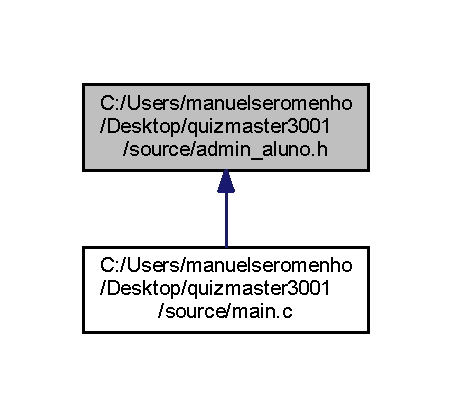
\includegraphics[width=217pt]{admin__aluno_8h__dep__incl}
\end{center}
\end{figure}
\subsection*{Functions}
\begin{DoxyCompactItemize}
\item 
void \hyperlink{admin__aluno_8h_a5ca8c98e0ec07103720da6e2b8241eac}{intro} (void)
\begin{DoxyCompactList}\small\item\em Menu de Login. \end{DoxyCompactList}\item 
void \hyperlink{admin__aluno_8h_a0eac57f91f15716c9f3e15c935c69a8a}{admin} (\hyperlink{structalunotab}{alunotab} $\ast$alu)
\begin{DoxyCompactList}\small\item\em Menu Administrador. \end{DoxyCompactList}\item 
void \hyperlink{admin__aluno_8h_a492a0d7c8e5e95d782d96e3b29109b4a}{leraluno} (\hyperlink{structalunotab}{alunotab} $\ast$x)
\begin{DoxyCompactList}\small\item\em funcao para ler do ficheiro do aluno/user \end{DoxyCompactList}\item 
void \hyperlink{admin__aluno_8h_a95ea7a920a9f3bbd4376f2ca5ae24e9b}{inserir\+Aluno} (\hyperlink{structalunotab}{alunotab} $\ast$x)
\begin{DoxyCompactList}\small\item\em fun��o para inserir novos alunos \end{DoxyCompactList}\item 
void \hyperlink{admin__aluno_8h_a1bbc96567c4165ce3093566cf12a8d83}{consultar\+Aluno} (\hyperlink{structalunotab}{alunotab} $\ast$x)
\begin{DoxyCompactList}\small\item\em funcao para consultar os alunos \end{DoxyCompactList}\item 
int \hyperlink{admin__aluno_8h_afe4837590a9a74173a073ddba2f88d02}{elim\+Alunos} (\hyperlink{structalunotab}{alunotab} $\ast$x)
\begin{DoxyCompactList}\small\item\em fun��o para eliminar os alunos \end{DoxyCompactList}\item 
void \hyperlink{admin__aluno_8h_acf884dc8124dd4077bc0d46708bacb35}{edit\+Aluno} (\hyperlink{structalunotab}{alunotab} $\ast$x)
\begin{DoxyCompactList}\small\item\em fun��o para editar alunos \end{DoxyCompactList}\item 
void \hyperlink{admin__aluno_8h_a5d3cb89467dc410ceb1ded2692ea1e1a}{gravar\+Aluno} (\hyperlink{structalunotab}{alunotab} $\ast$x)
\begin{DoxyCompactList}\small\item\em fun��o para gravar \end{DoxyCompactList}\item 
void \hyperlink{admin__aluno_8h_adddc3998ca213a8620431d4d50a4ac1b}{gest\+\_\+alunos} (\hyperlink{structalunotab}{alunotab} $\ast$alu)
\begin{DoxyCompactList}\small\item\em fun��o gestao de alunos \end{DoxyCompactList}\end{DoxyCompactItemize}


\subsection{Function Documentation}
\hypertarget{admin__aluno_8h_a0eac57f91f15716c9f3e15c935c69a8a}{\index{admin\+\_\+aluno.\+h@{admin\+\_\+aluno.\+h}!admin@{admin}}
\index{admin@{admin}!admin\+\_\+aluno.\+h@{admin\+\_\+aluno.\+h}}
\subsubsection[{admin}]{\setlength{\rightskip}{0pt plus 5cm}void admin (
\begin{DoxyParamCaption}
\item[{{\bf alunotab} $\ast$}]{alu}
\end{DoxyParamCaption}
)}}\label{admin__aluno_8h_a0eac57f91f15716c9f3e15c935c69a8a}


Menu Administrador. 

funcao do menu Administrador 
\begin{DoxyParams}{Parameters}
{\em $\ast$alu} & \+: alunotab \\
\hline
\end{DoxyParams}


Here is the call graph for this function\+:\nopagebreak
\begin{figure}[H]
\begin{center}
\leavevmode
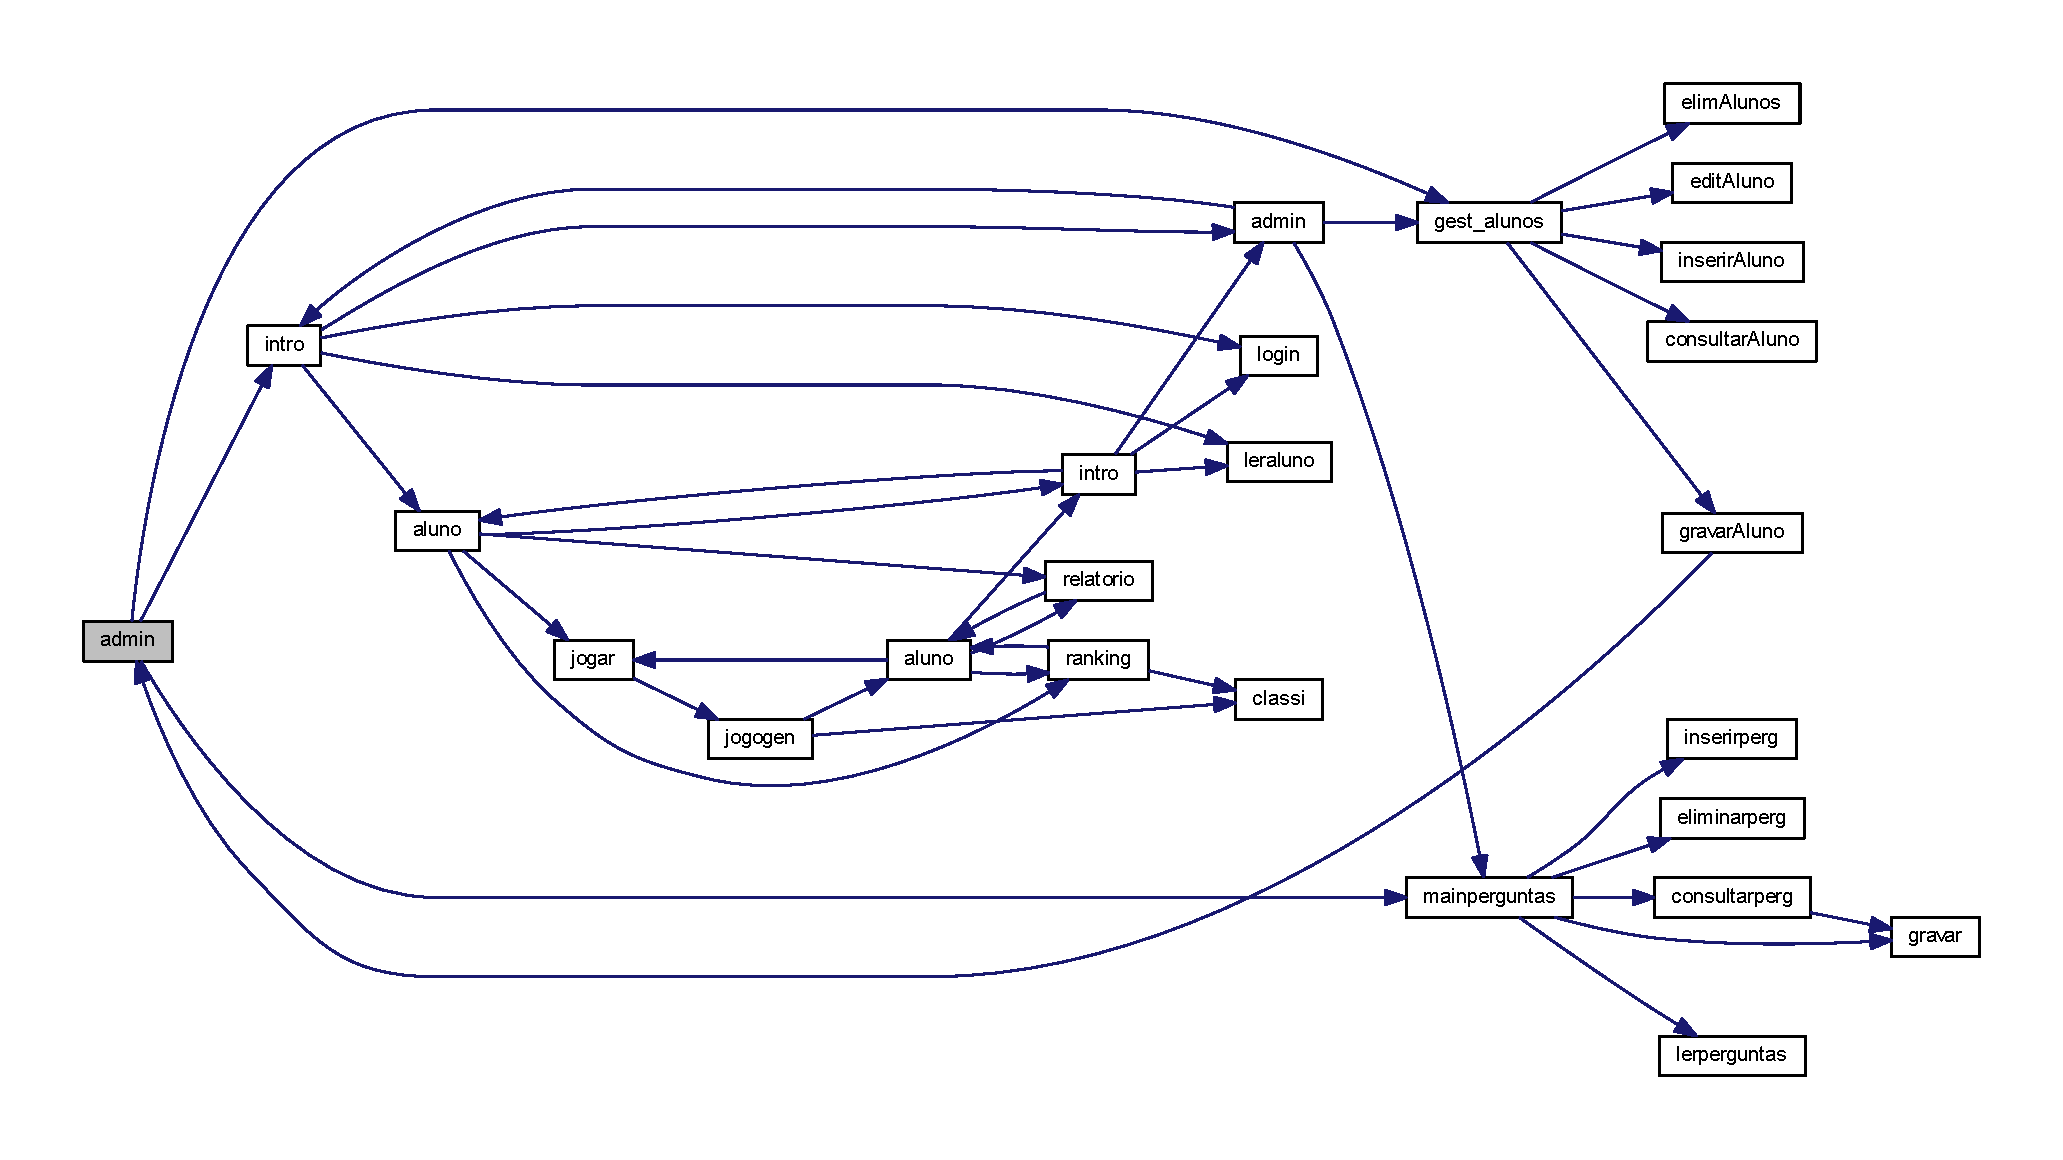
\includegraphics[width=350pt]{admin__aluno_8h_a0eac57f91f15716c9f3e15c935c69a8a_cgraph}
\end{center}
\end{figure}




Here is the caller graph for this function\+:\nopagebreak
\begin{figure}[H]
\begin{center}
\leavevmode
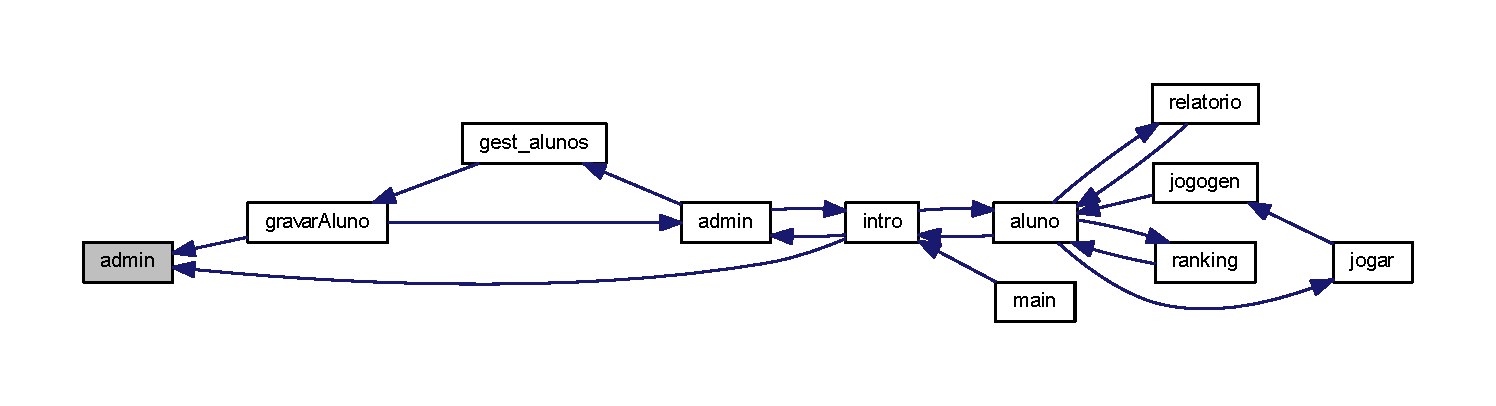
\includegraphics[width=350pt]{admin__aluno_8h_a0eac57f91f15716c9f3e15c935c69a8a_icgraph}
\end{center}
\end{figure}


\hypertarget{admin__aluno_8h_a1bbc96567c4165ce3093566cf12a8d83}{\index{admin\+\_\+aluno.\+h@{admin\+\_\+aluno.\+h}!consultar\+Aluno@{consultar\+Aluno}}
\index{consultar\+Aluno@{consultar\+Aluno}!admin\+\_\+aluno.\+h@{admin\+\_\+aluno.\+h}}
\subsubsection[{consultar\+Aluno}]{\setlength{\rightskip}{0pt plus 5cm}void consultar\+Aluno (
\begin{DoxyParamCaption}
\item[{{\bf alunotab} $\ast$}]{x}
\end{DoxyParamCaption}
)}}\label{admin__aluno_8h_a1bbc96567c4165ce3093566cf12a8d83}


funcao para consultar os alunos 

funcao Consultar Alunos Funcao que permite consultar todos os alunos j� inseridos 
\begin{DoxyParams}{Parameters}
{\em $\ast$x} & \+: alunotab \\
\hline
\end{DoxyParams}


Here is the caller graph for this function\+:\nopagebreak
\begin{figure}[H]
\begin{center}
\leavevmode
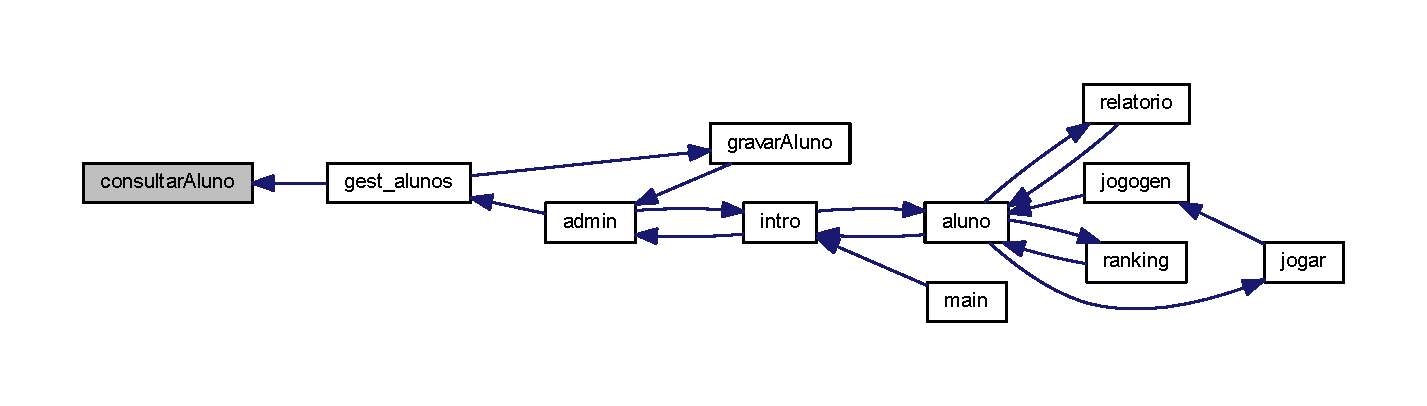
\includegraphics[width=350pt]{admin__aluno_8h_a1bbc96567c4165ce3093566cf12a8d83_icgraph}
\end{center}
\end{figure}


\hypertarget{admin__aluno_8h_acf884dc8124dd4077bc0d46708bacb35}{\index{admin\+\_\+aluno.\+h@{admin\+\_\+aluno.\+h}!edit\+Aluno@{edit\+Aluno}}
\index{edit\+Aluno@{edit\+Aluno}!admin\+\_\+aluno.\+h@{admin\+\_\+aluno.\+h}}
\subsubsection[{edit\+Aluno}]{\setlength{\rightskip}{0pt plus 5cm}void edit\+Aluno (
\begin{DoxyParamCaption}
\item[{{\bf alunotab} $\ast$}]{x}
\end{DoxyParamCaption}
)}}\label{admin__aluno_8h_acf884dc8124dd4077bc0d46708bacb35}


fun��o para editar alunos 

funcao editar aluno Funcao para editar as passwords e turmas dos alunos 
\begin{DoxyParams}{Parameters}
{\em $\ast$x} & \+: alunotab \\
\hline
\end{DoxyParams}
\begin{DoxyReturn}{Returns}
void 
\end{DoxyReturn}


Here is the caller graph for this function\+:\nopagebreak
\begin{figure}[H]
\begin{center}
\leavevmode
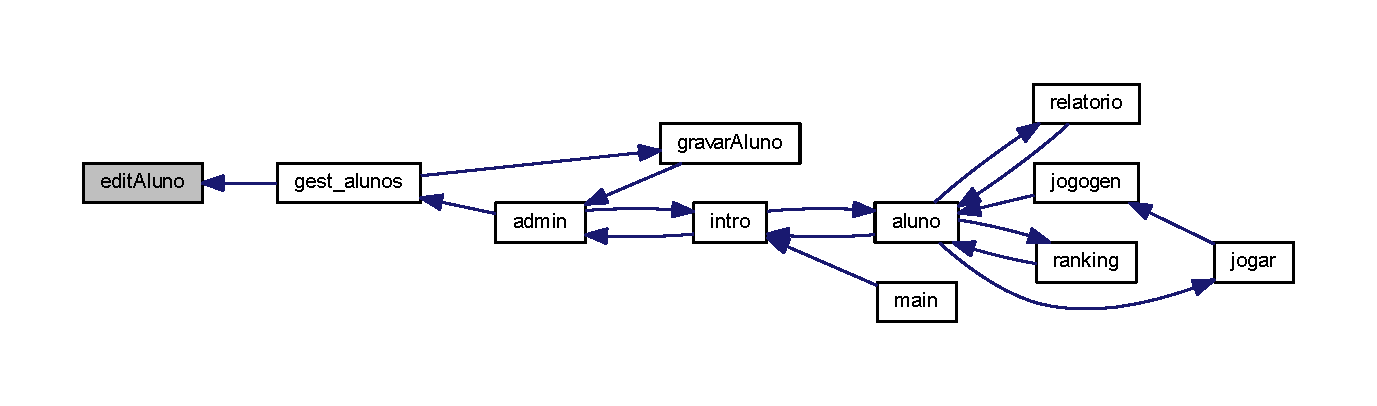
\includegraphics[width=350pt]{admin__aluno_8h_acf884dc8124dd4077bc0d46708bacb35_icgraph}
\end{center}
\end{figure}


\hypertarget{admin__aluno_8h_afe4837590a9a74173a073ddba2f88d02}{\index{admin\+\_\+aluno.\+h@{admin\+\_\+aluno.\+h}!elim\+Alunos@{elim\+Alunos}}
\index{elim\+Alunos@{elim\+Alunos}!admin\+\_\+aluno.\+h@{admin\+\_\+aluno.\+h}}
\subsubsection[{elim\+Alunos}]{\setlength{\rightskip}{0pt plus 5cm}int elim\+Alunos (
\begin{DoxyParamCaption}
\item[{{\bf alunotab} $\ast$}]{x}
\end{DoxyParamCaption}
)}}\label{admin__aluno_8h_afe4837590a9a74173a073ddba2f88d02}


fun��o para eliminar os alunos 

funcao eliminar alunos/users Funcao para eliminar alunos que estejam presentes na memoria 
\begin{DoxyParams}{Parameters}
{\em $\ast$x} & \+: alunotab \\
\hline
\end{DoxyParams}
\begin{DoxyReturn}{Returns}
elim\+Alunos\+: int 
\end{DoxyReturn}


Here is the caller graph for this function\+:\nopagebreak
\begin{figure}[H]
\begin{center}
\leavevmode
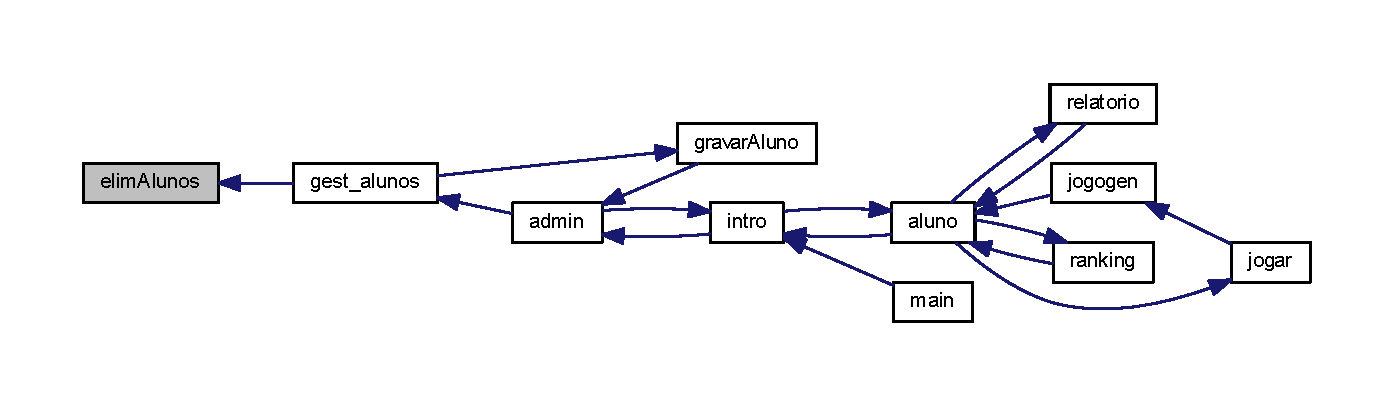
\includegraphics[width=350pt]{admin__aluno_8h_afe4837590a9a74173a073ddba2f88d02_icgraph}
\end{center}
\end{figure}


\hypertarget{admin__aluno_8h_adddc3998ca213a8620431d4d50a4ac1b}{\index{admin\+\_\+aluno.\+h@{admin\+\_\+aluno.\+h}!gest\+\_\+alunos@{gest\+\_\+alunos}}
\index{gest\+\_\+alunos@{gest\+\_\+alunos}!admin\+\_\+aluno.\+h@{admin\+\_\+aluno.\+h}}
\subsubsection[{gest\+\_\+alunos}]{\setlength{\rightskip}{0pt plus 5cm}void gest\+\_\+alunos (
\begin{DoxyParamCaption}
\item[{{\bf alunotab} $\ast$}]{alu}
\end{DoxyParamCaption}
)}}\label{admin__aluno_8h_adddc3998ca213a8620431d4d50a4ac1b}


fun��o gestao de alunos 

funcao gest�o de alunos Funcao do menu gest�o de alunos, contendo as v�rias op��es de gest�o do aluno 
\begin{DoxyParams}{Parameters}
{\em $\ast$alu} & \+: alunotab \\
\hline
\end{DoxyParams}
\begin{DoxyReturn}{Returns}
void 
\end{DoxyReturn}


Here is the call graph for this function\+:\nopagebreak
\begin{figure}[H]
\begin{center}
\leavevmode
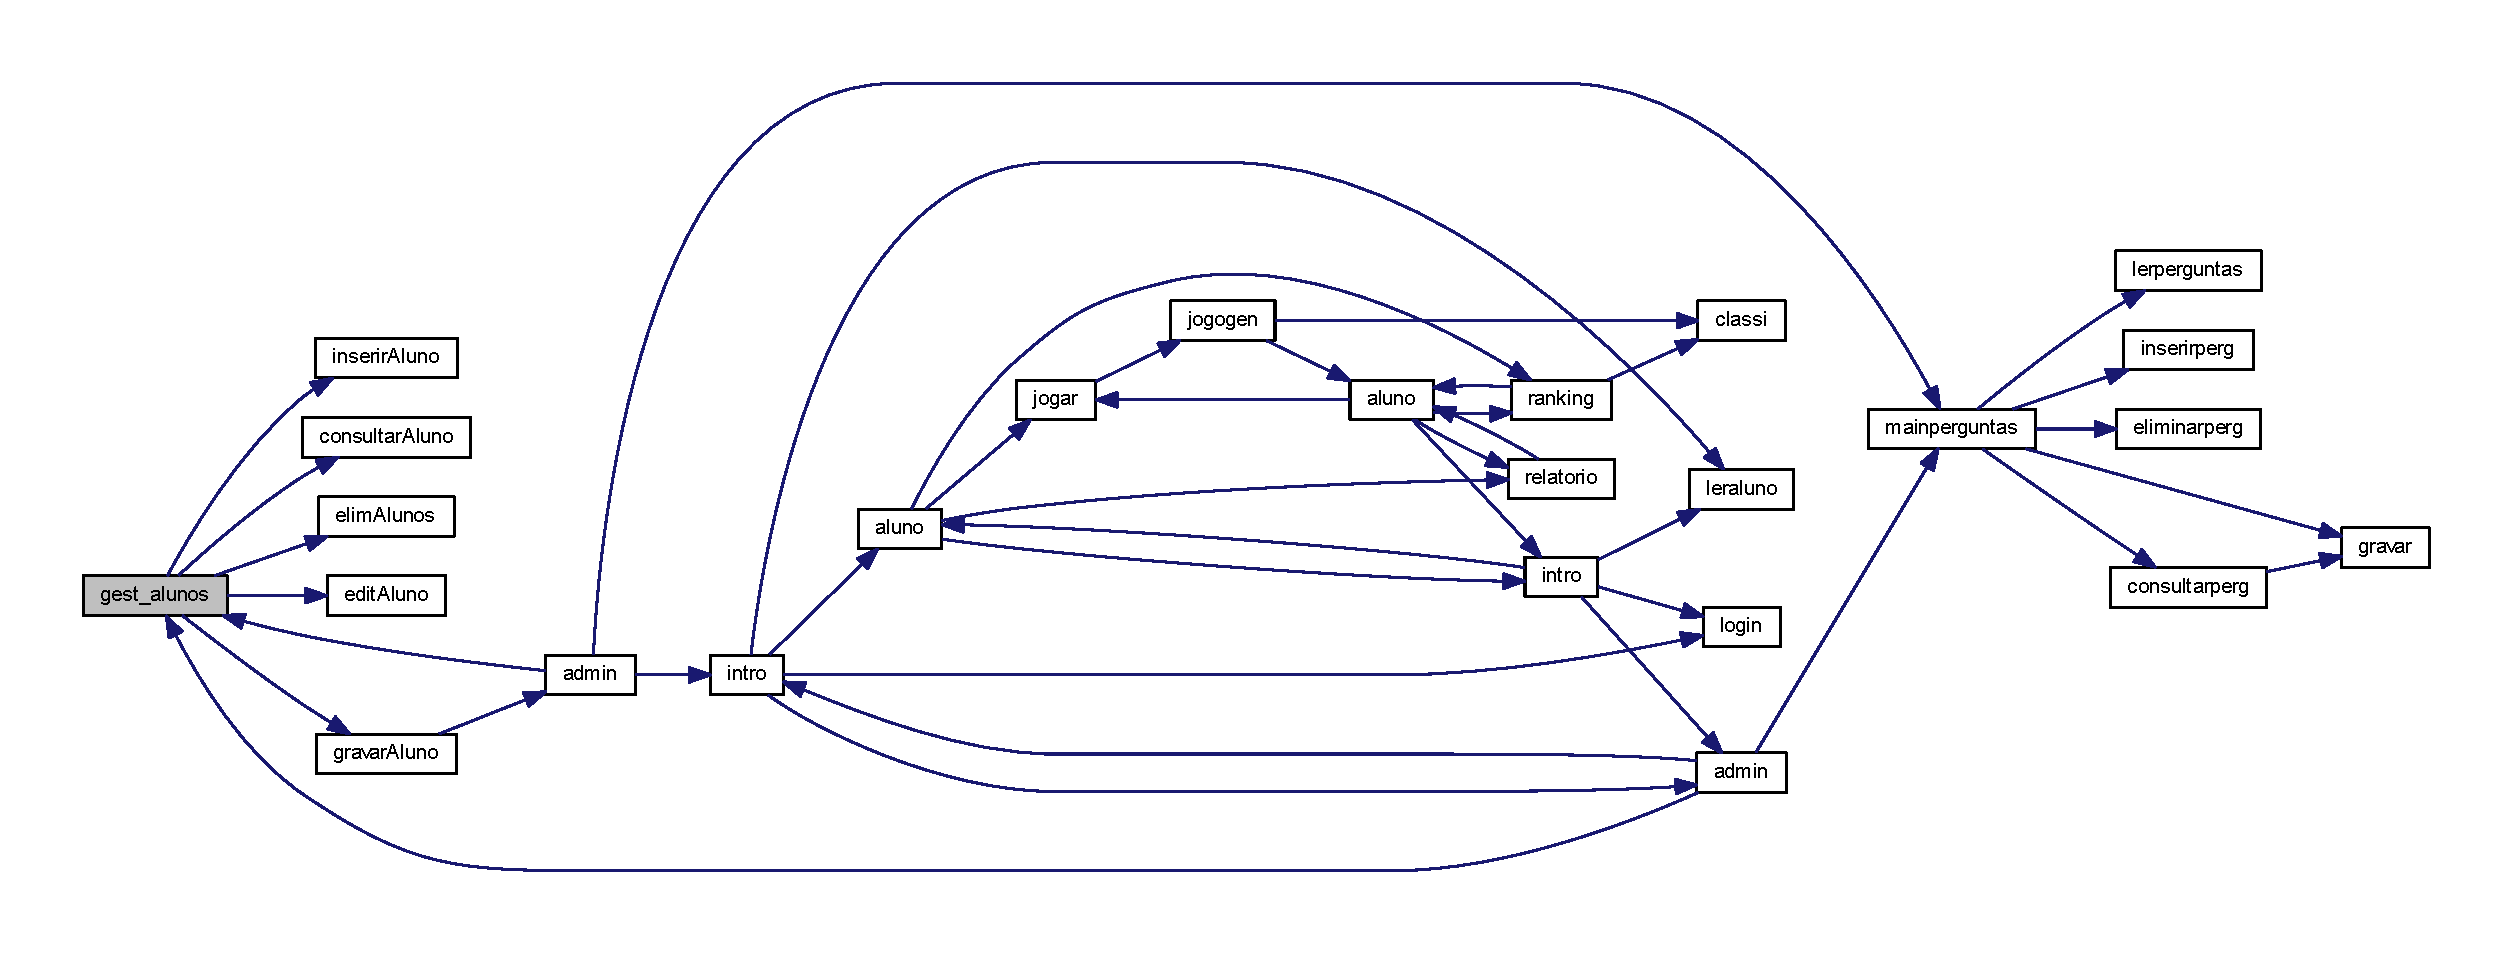
\includegraphics[width=350pt]{admin__aluno_8h_adddc3998ca213a8620431d4d50a4ac1b_cgraph}
\end{center}
\end{figure}




Here is the caller graph for this function\+:\nopagebreak
\begin{figure}[H]
\begin{center}
\leavevmode
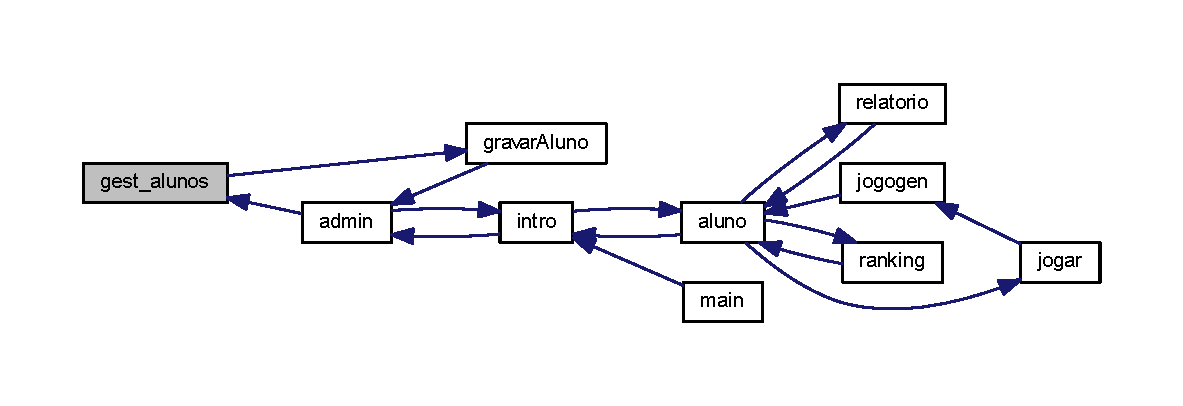
\includegraphics[width=350pt]{admin__aluno_8h_adddc3998ca213a8620431d4d50a4ac1b_icgraph}
\end{center}
\end{figure}


\hypertarget{admin__aluno_8h_a5d3cb89467dc410ceb1ded2692ea1e1a}{\index{admin\+\_\+aluno.\+h@{admin\+\_\+aluno.\+h}!gravar\+Aluno@{gravar\+Aluno}}
\index{gravar\+Aluno@{gravar\+Aluno}!admin\+\_\+aluno.\+h@{admin\+\_\+aluno.\+h}}
\subsubsection[{gravar\+Aluno}]{\setlength{\rightskip}{0pt plus 5cm}void gravar\+Aluno (
\begin{DoxyParamCaption}
\item[{{\bf alunotab} $\ast$}]{x}
\end{DoxyParamCaption}
)}}\label{admin__aluno_8h_a5d3cb89467dc410ceb1ded2692ea1e1a}


fun��o para gravar 

funcao gravar aluno Funcao para gravar todos os alunos da memoria para um ficheiro .txt 
\begin{DoxyParams}{Parameters}
{\em $\ast$x} & \+: alunotab \\
\hline
\end{DoxyParams}
\begin{DoxyReturn}{Returns}
void 
\end{DoxyReturn}


Here is the call graph for this function\+:\nopagebreak
\begin{figure}[H]
\begin{center}
\leavevmode
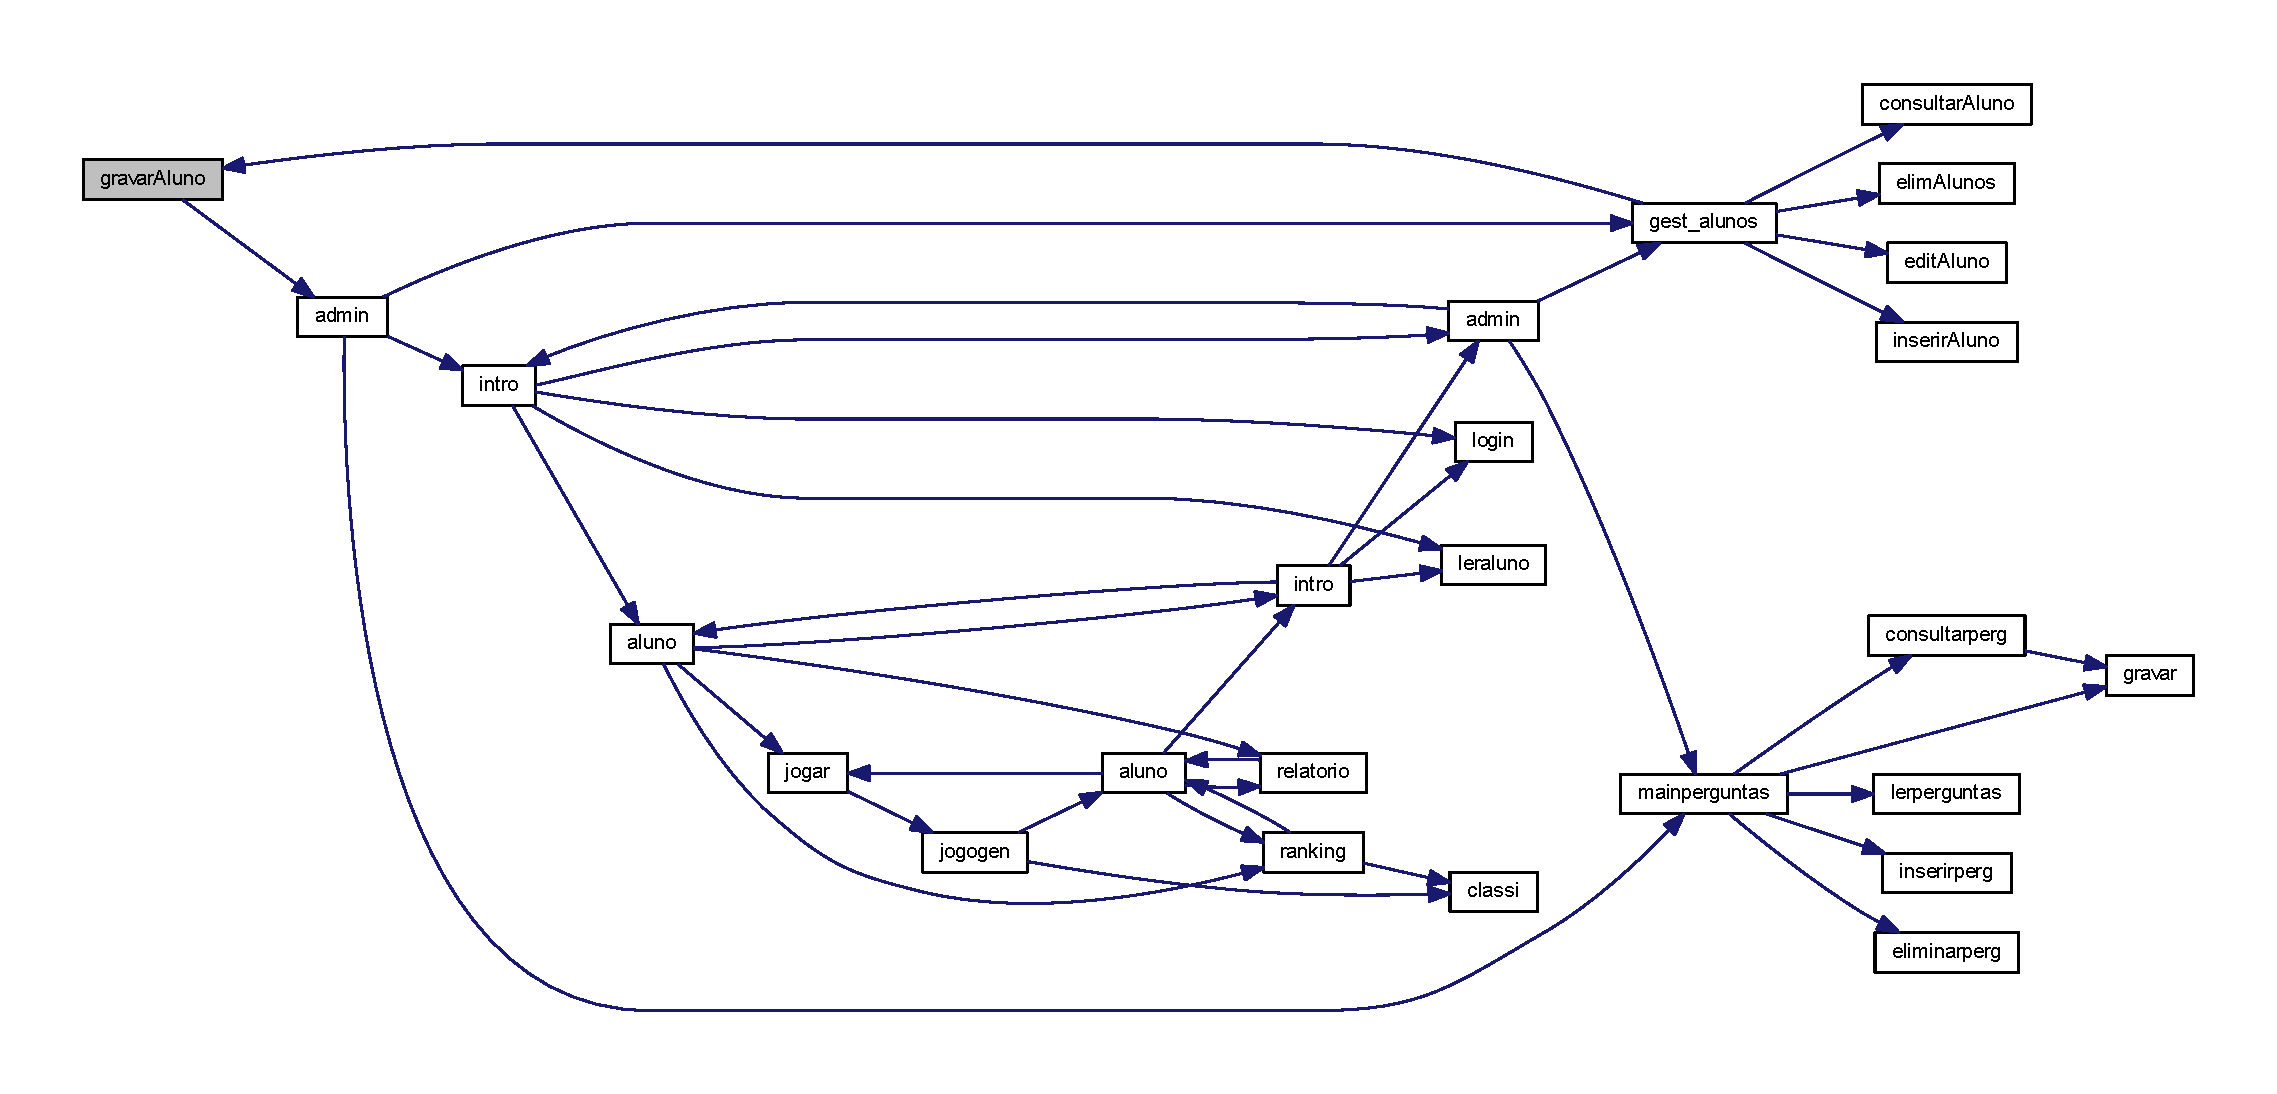
\includegraphics[width=350pt]{admin__aluno_8h_a5d3cb89467dc410ceb1ded2692ea1e1a_cgraph}
\end{center}
\end{figure}




Here is the caller graph for this function\+:\nopagebreak
\begin{figure}[H]
\begin{center}
\leavevmode
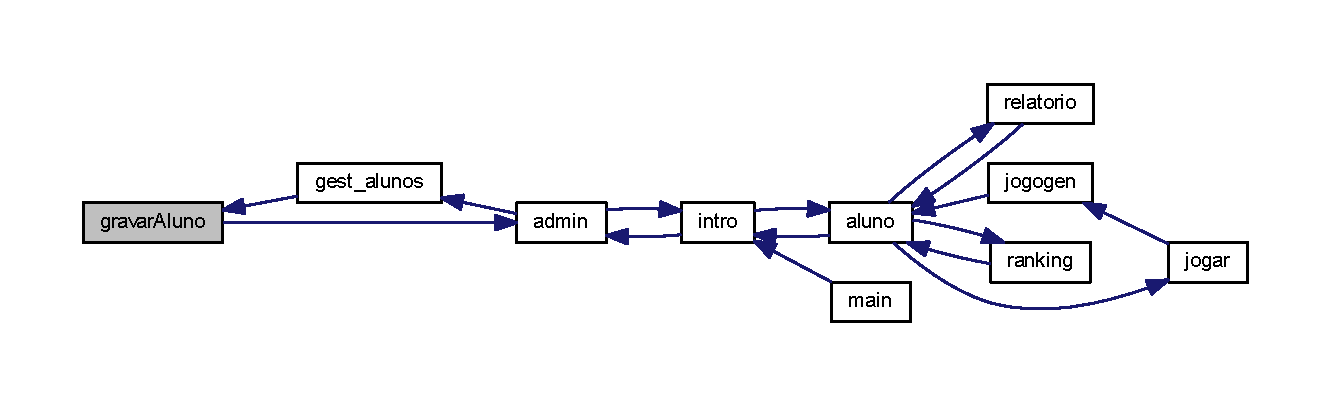
\includegraphics[width=350pt]{admin__aluno_8h_a5d3cb89467dc410ceb1ded2692ea1e1a_icgraph}
\end{center}
\end{figure}


\hypertarget{admin__aluno_8h_a95ea7a920a9f3bbd4376f2ca5ae24e9b}{\index{admin\+\_\+aluno.\+h@{admin\+\_\+aluno.\+h}!inserir\+Aluno@{inserir\+Aluno}}
\index{inserir\+Aluno@{inserir\+Aluno}!admin\+\_\+aluno.\+h@{admin\+\_\+aluno.\+h}}
\subsubsection[{inserir\+Aluno}]{\setlength{\rightskip}{0pt plus 5cm}void inserir\+Aluno (
\begin{DoxyParamCaption}
\item[{{\bf alunotab} $\ast$}]{x}
\end{DoxyParamCaption}
)}}\label{admin__aluno_8h_a95ea7a920a9f3bbd4376f2ca5ae24e9b}


fun��o para inserir novos alunos 

Funcao de Insercao de Alunos/\+Users Fun��o para inserir novos alunos 
\begin{DoxyParams}{Parameters}
{\em $\ast$x} & \+: alunotab \\
\hline
\end{DoxyParams}


Here is the caller graph for this function\+:\nopagebreak
\begin{figure}[H]
\begin{center}
\leavevmode
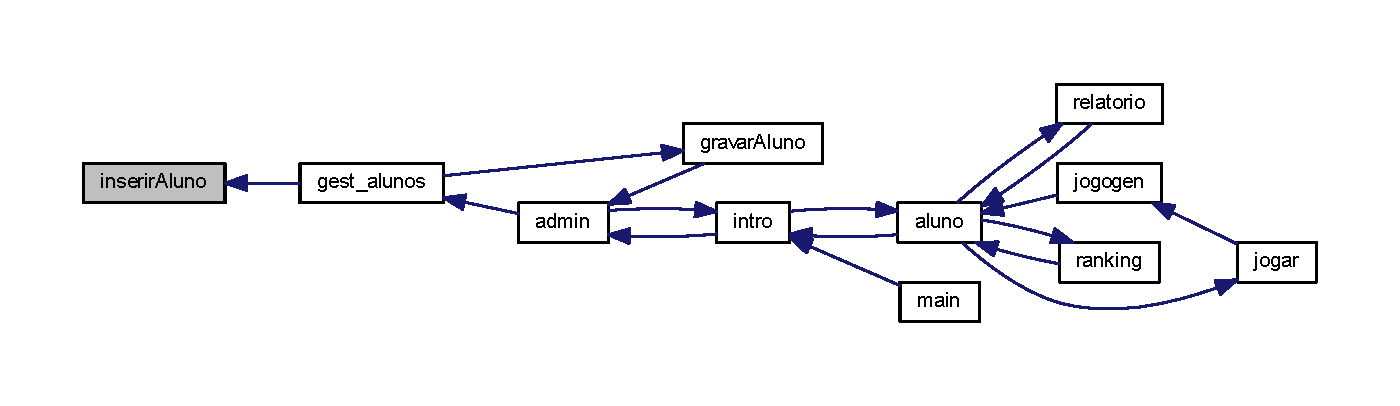
\includegraphics[width=350pt]{admin__aluno_8h_a95ea7a920a9f3bbd4376f2ca5ae24e9b_icgraph}
\end{center}
\end{figure}


\hypertarget{admin__aluno_8h_a5ca8c98e0ec07103720da6e2b8241eac}{\index{admin\+\_\+aluno.\+h@{admin\+\_\+aluno.\+h}!intro@{intro}}
\index{intro@{intro}!admin\+\_\+aluno.\+h@{admin\+\_\+aluno.\+h}}
\subsubsection[{intro}]{\setlength{\rightskip}{0pt plus 5cm}void intro (
\begin{DoxyParamCaption}
\item[{void}]{}
\end{DoxyParamCaption}
)}}\label{admin__aluno_8h_a5ca8c98e0ec07103720da6e2b8241eac}


Menu de Login. 

funcao do Menu de Login (onde os users/alunos introduzem a informa��o para ser verificada pela fun��o login) 

Here is the call graph for this function\+:\nopagebreak
\begin{figure}[H]
\begin{center}
\leavevmode
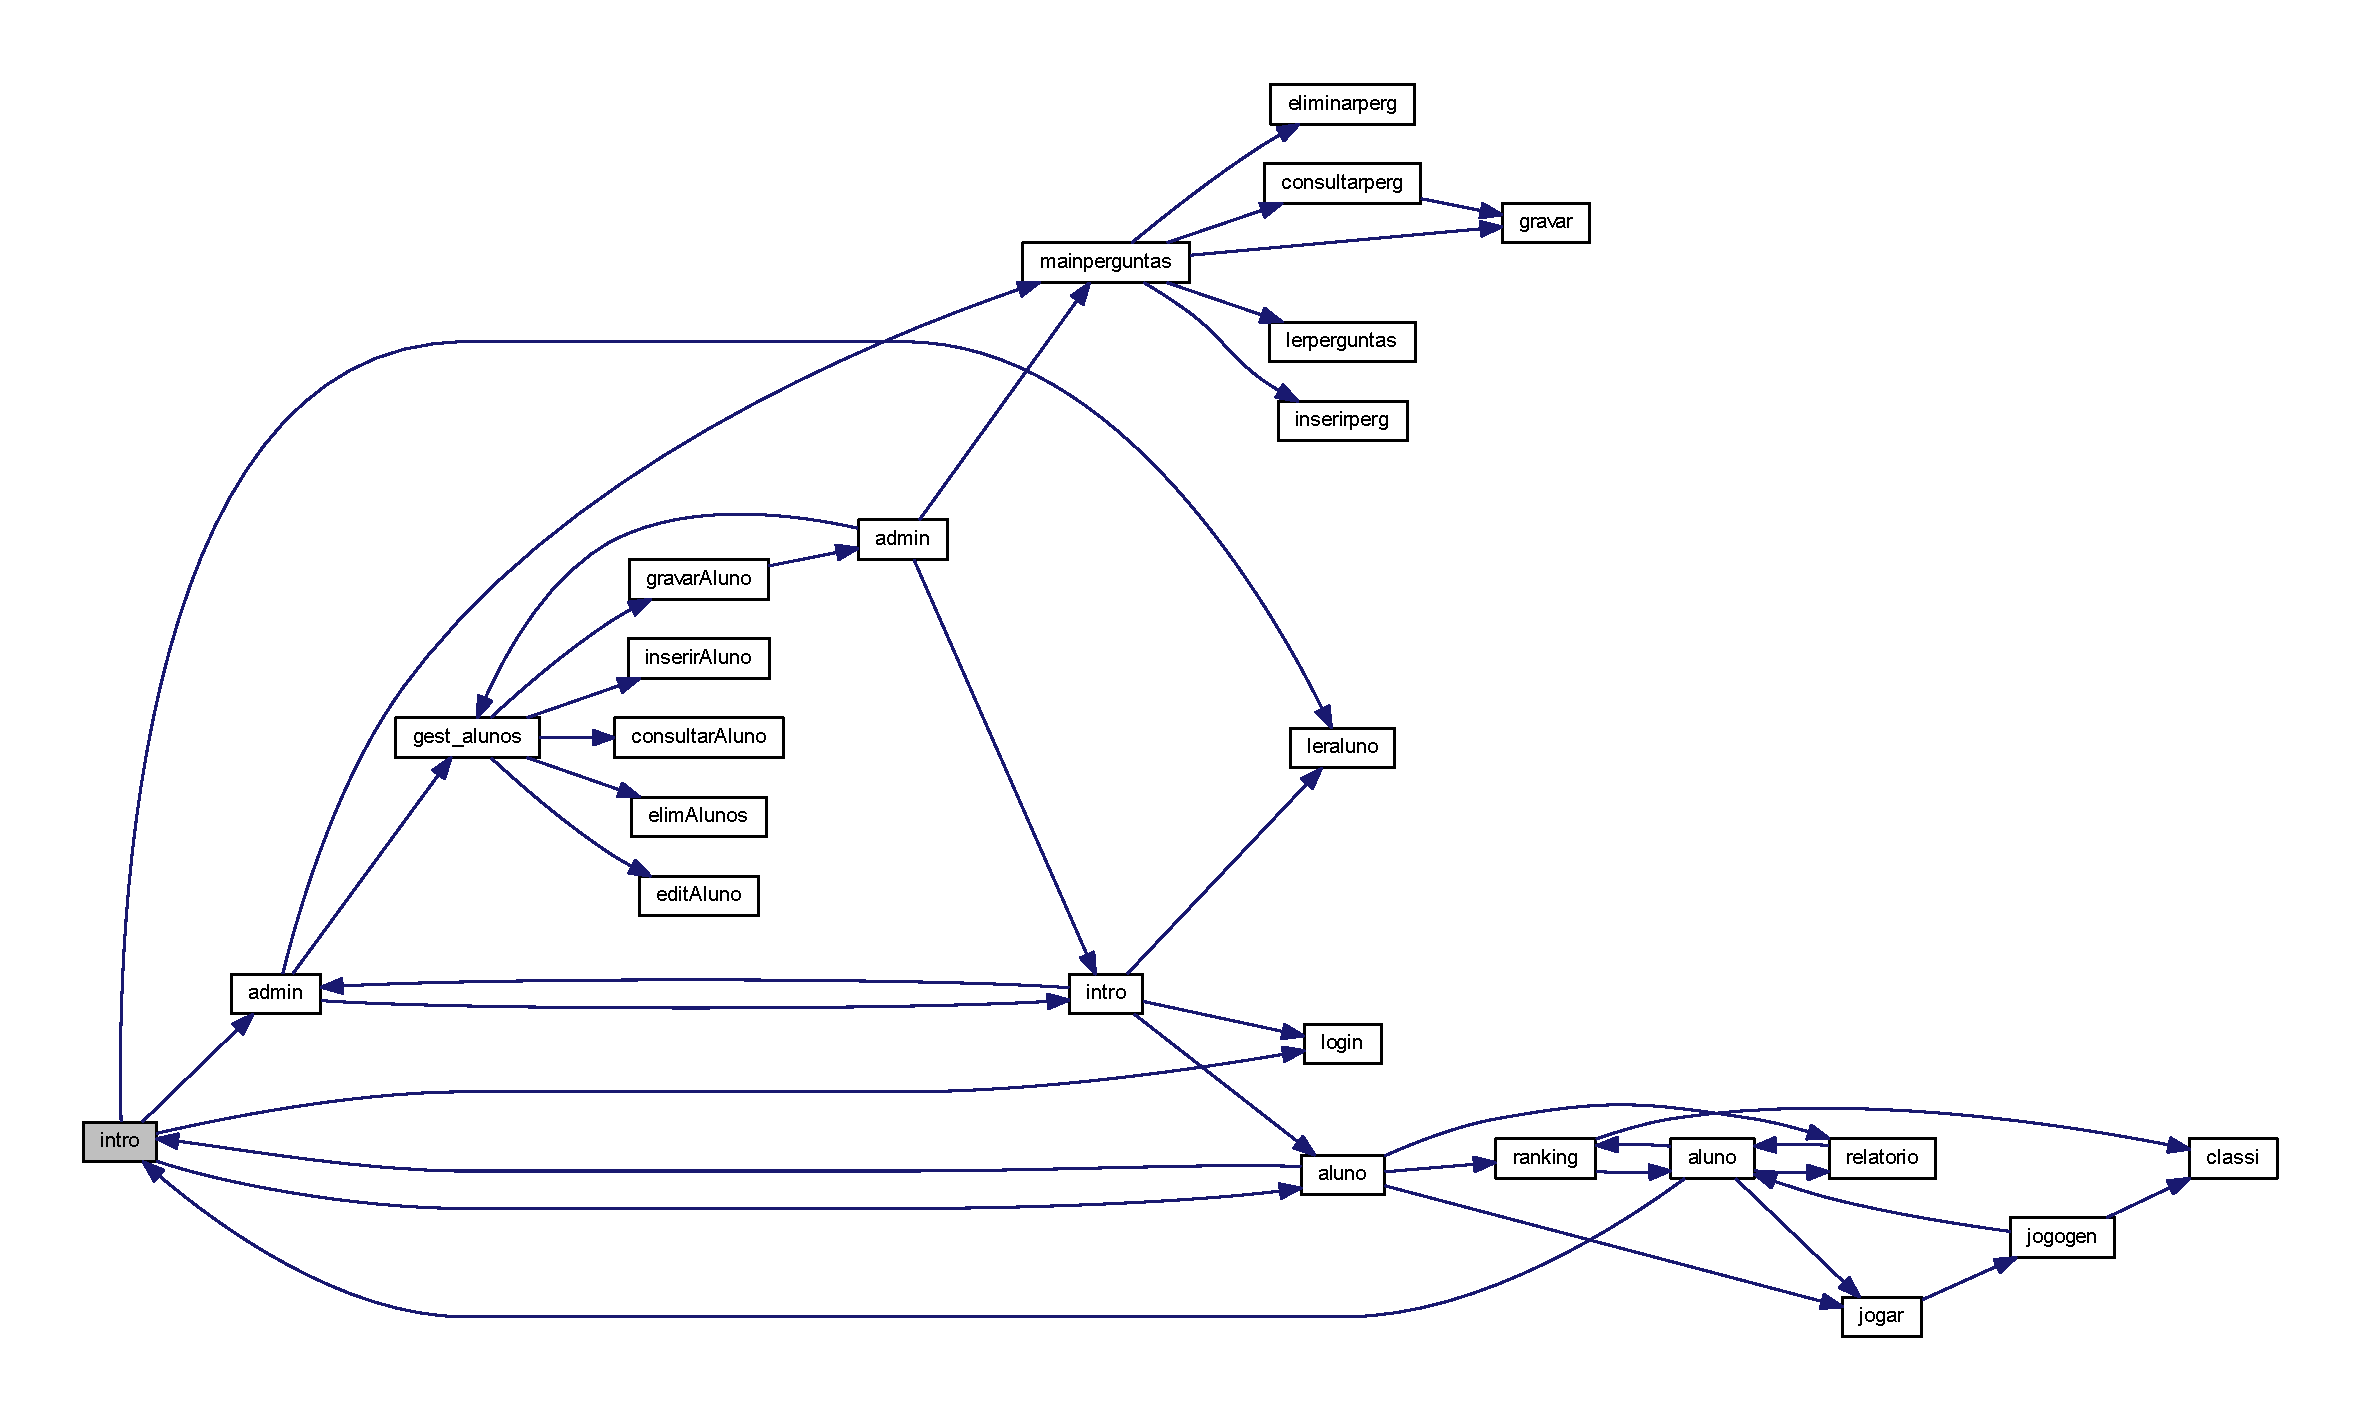
\includegraphics[width=350pt]{admin__aluno_8h_a5ca8c98e0ec07103720da6e2b8241eac_cgraph}
\end{center}
\end{figure}




Here is the caller graph for this function\+:\nopagebreak
\begin{figure}[H]
\begin{center}
\leavevmode
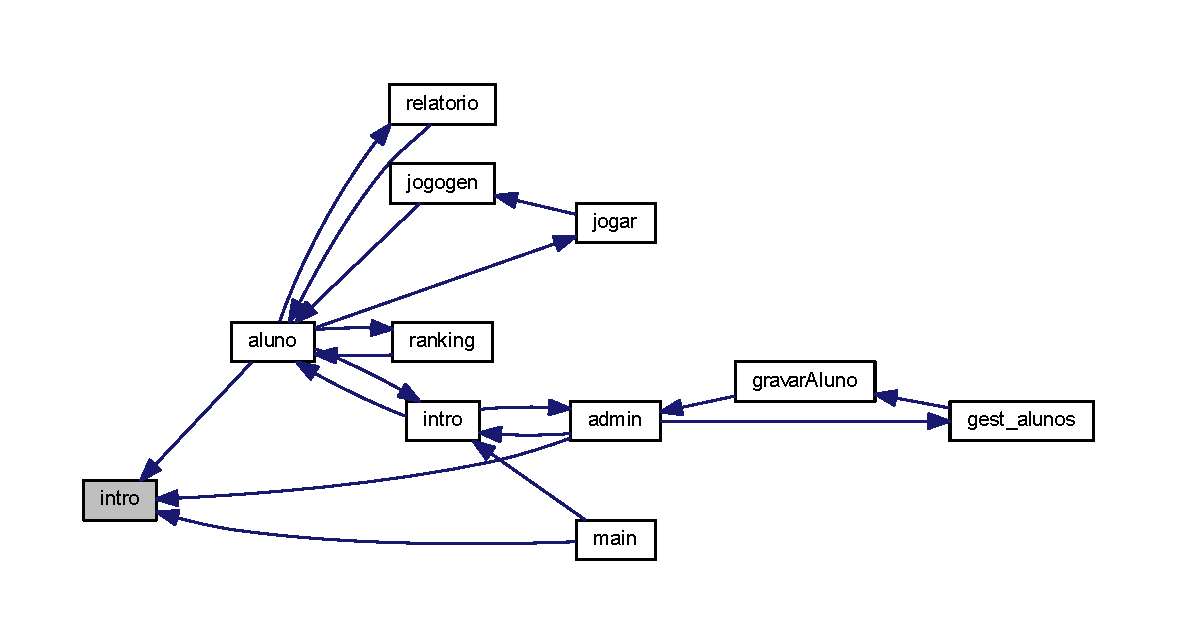
\includegraphics[width=350pt]{admin__aluno_8h_a5ca8c98e0ec07103720da6e2b8241eac_icgraph}
\end{center}
\end{figure}


\hypertarget{admin__aluno_8h_a492a0d7c8e5e95d782d96e3b29109b4a}{\index{admin\+\_\+aluno.\+h@{admin\+\_\+aluno.\+h}!leraluno@{leraluno}}
\index{leraluno@{leraluno}!admin\+\_\+aluno.\+h@{admin\+\_\+aluno.\+h}}
\subsubsection[{leraluno}]{\setlength{\rightskip}{0pt plus 5cm}void leraluno (
\begin{DoxyParamCaption}
\item[{{\bf alunotab} $\ast$}]{x}
\end{DoxyParamCaption}
)}}\label{admin__aluno_8h_a492a0d7c8e5e95d782d96e3b29109b4a}


funcao para ler do ficheiro do aluno/user 

funcao ler aluno esta fun��o ir� ler de um ficheiro .txt todos os alunos/user j� inseridos e passar para a memoria 
\begin{DoxyParams}{Parameters}
{\em $\ast$x} & \+: alunotab \\
\hline
\end{DoxyParams}


Here is the caller graph for this function\+:\nopagebreak
\begin{figure}[H]
\begin{center}
\leavevmode
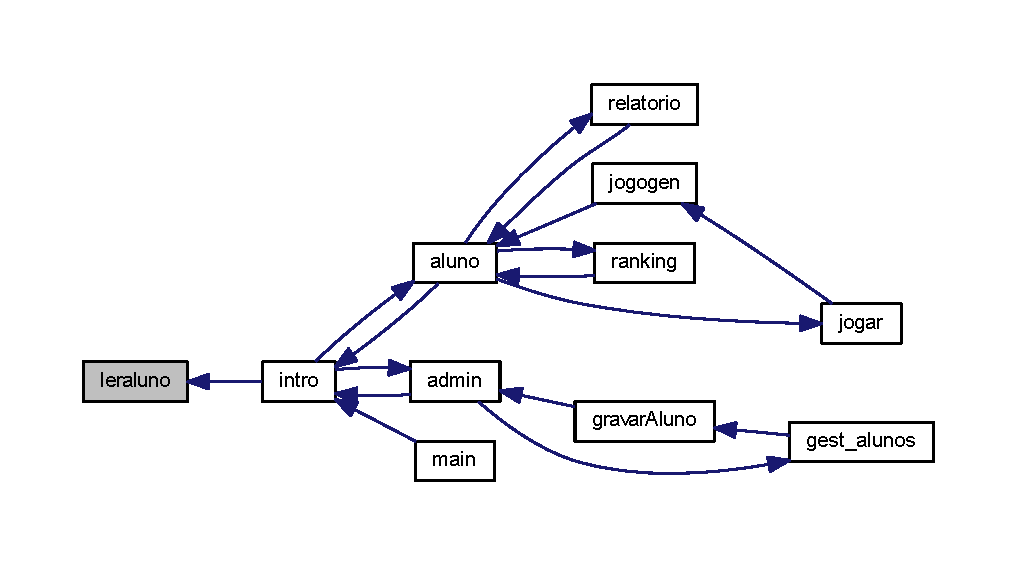
\includegraphics[width=350pt]{admin__aluno_8h_a492a0d7c8e5e95d782d96e3b29109b4a_icgraph}
\end{center}
\end{figure}



\hypertarget{admin__perguntas_8h}{\section{C\+:/\+Users/manuelseromenho/\+Desktop/quizmaster3001/source/admin\+\_\+perguntas.h File Reference}
\label{admin__perguntas_8h}\index{C\+:/\+Users/manuelseromenho/\+Desktop/quizmaster3001/source/admin\+\_\+perguntas.\+h@{C\+:/\+Users/manuelseromenho/\+Desktop/quizmaster3001/source/admin\+\_\+perguntas.\+h}}
}
This graph shows which files directly or indirectly include this file\+:\nopagebreak
\begin{figure}[H]
\begin{center}
\leavevmode
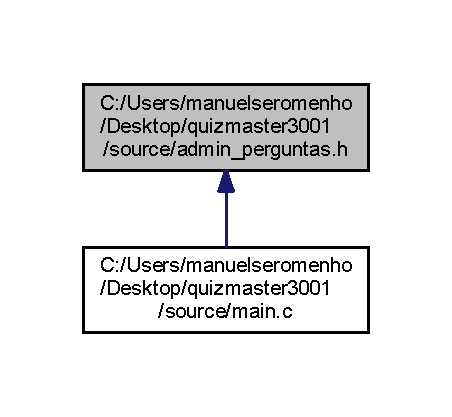
\includegraphics[width=217pt]{admin__perguntas_8h__dep__incl}
\end{center}
\end{figure}
\subsection*{Functions}
\begin{DoxyCompactItemize}
\item 
void \hyperlink{admin__perguntas_8h_a579492a6090f14af5ca1018dc507e3db}{gravar} (\hyperlink{structperguntas}{perguntas} $\ast$x)
\begin{DoxyCompactList}\small\item\em funcao para gravar no ficheiro \end{DoxyCompactList}\item 
void \hyperlink{admin__perguntas_8h_a273151aa6319565d10bb075007dcc3a9}{inserirperg} (\hyperlink{structperguntas}{perguntas} $\ast$x)
\begin{DoxyCompactList}\small\item\em funcao para inserir perguntas \end{DoxyCompactList}\item 
void \hyperlink{admin__perguntas_8h_a5307a3752b688902193da2e92fc86109}{consultarperg} (\hyperlink{structperguntas}{perguntas} $\ast$x)
\begin{DoxyCompactList}\small\item\em funcao para consultar perguntas \end{DoxyCompactList}\item 
int \hyperlink{admin__perguntas_8h_a3d87d64c49b1c5769f6febdacb72f96d}{eliminarperg} (\hyperlink{structperguntas}{perguntas} $\ast$x)
\begin{DoxyCompactList}\small\item\em fun�ao para eliminar perguntas \end{DoxyCompactList}\item 
void \hyperlink{admin__perguntas_8h_a921c1f88176bd80774d8d1eaa3a80002}{lerperguntas} (\hyperlink{structperguntas}{perguntas} $\ast$x)
\begin{DoxyCompactList}\small\item\em funcao para ler o ficheiro de perguntas \end{DoxyCompactList}\item 
\hyperlink{admin__perguntas_8h_a7ab3ce3466d990aa0d1f85a5d15a6716}{mainperguntas} ()
\begin{DoxyCompactList}\small\item\em Menu de Perguntas. \end{DoxyCompactList}\end{DoxyCompactItemize}


\subsection{Function Documentation}
\hypertarget{admin__perguntas_8h_a5307a3752b688902193da2e92fc86109}{\index{admin\+\_\+perguntas.\+h@{admin\+\_\+perguntas.\+h}!consultarperg@{consultarperg}}
\index{consultarperg@{consultarperg}!admin\+\_\+perguntas.\+h@{admin\+\_\+perguntas.\+h}}
\subsubsection[{consultarperg}]{\setlength{\rightskip}{0pt plus 5cm}void consultarperg (
\begin{DoxyParamCaption}
\item[{{\bf perguntas} $\ast$}]{x}
\end{DoxyParamCaption}
)}}\label{admin__perguntas_8h_a5307a3752b688902193da2e92fc86109}


funcao para consultar perguntas 

\textbackslash{} esta fun��o ir� permitir consultar as perguntas com base no ficheiro existente \textbackslash{} recebe o parametro de entrada \char`\"{}perguntas\char`\"{}

Here is the call graph for this function\+:\nopagebreak
\begin{figure}[H]
\begin{center}
\leavevmode
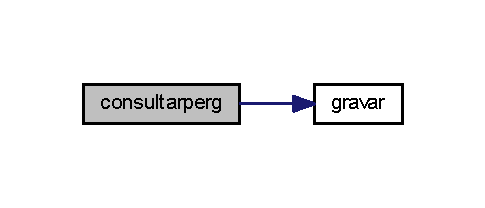
\includegraphics[width=233pt]{admin__perguntas_8h_a5307a3752b688902193da2e92fc86109_cgraph}
\end{center}
\end{figure}




Here is the caller graph for this function\+:\nopagebreak
\begin{figure}[H]
\begin{center}
\leavevmode
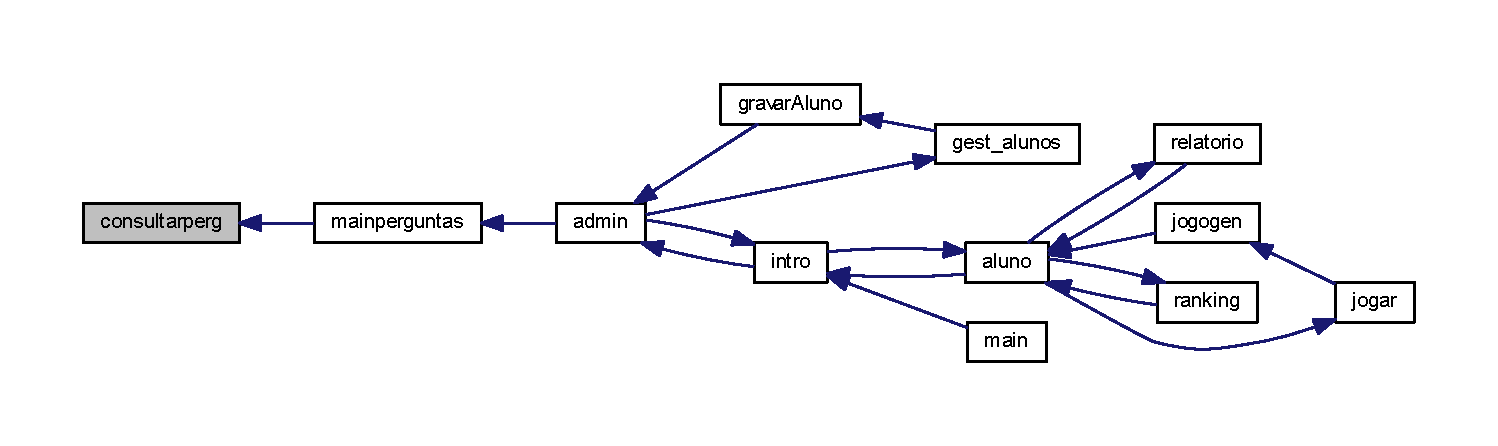
\includegraphics[width=350pt]{admin__perguntas_8h_a5307a3752b688902193da2e92fc86109_icgraph}
\end{center}
\end{figure}


\hypertarget{admin__perguntas_8h_a3d87d64c49b1c5769f6febdacb72f96d}{\index{admin\+\_\+perguntas.\+h@{admin\+\_\+perguntas.\+h}!eliminarperg@{eliminarperg}}
\index{eliminarperg@{eliminarperg}!admin\+\_\+perguntas.\+h@{admin\+\_\+perguntas.\+h}}
\subsubsection[{eliminarperg}]{\setlength{\rightskip}{0pt plus 5cm}int eliminarperg (
\begin{DoxyParamCaption}
\item[{{\bf perguntas} $\ast$}]{x}
\end{DoxyParamCaption}
)}}\label{admin__perguntas_8h_a3d87d64c49b1c5769f6febdacb72f96d}


fun�ao para eliminar perguntas 

\textbackslash{} esta fun��o ir� permitir eliminar perguntas \textbackslash{} recebe o parametro de entrada \char`\"{}perguntas\char`\"{} \begin{DoxyReturn}{Returns}
eliminarperg\+: int
\end{DoxyReturn}


Here is the caller graph for this function\+:\nopagebreak
\begin{figure}[H]
\begin{center}
\leavevmode
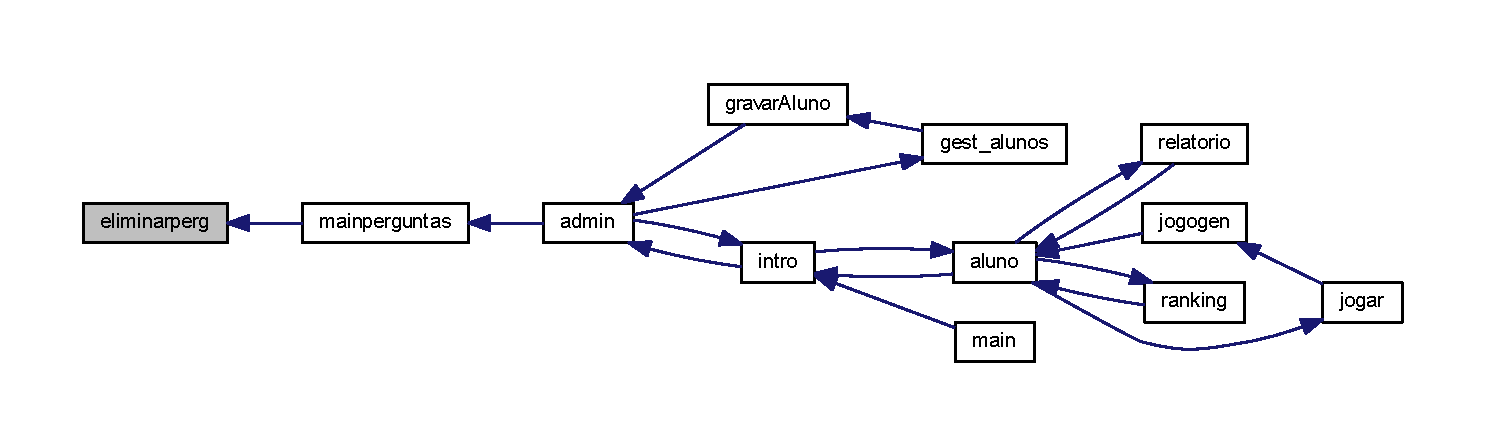
\includegraphics[width=350pt]{admin__perguntas_8h_a3d87d64c49b1c5769f6febdacb72f96d_icgraph}
\end{center}
\end{figure}


\hypertarget{admin__perguntas_8h_a579492a6090f14af5ca1018dc507e3db}{\index{admin\+\_\+perguntas.\+h@{admin\+\_\+perguntas.\+h}!gravar@{gravar}}
\index{gravar@{gravar}!admin\+\_\+perguntas.\+h@{admin\+\_\+perguntas.\+h}}
\subsubsection[{gravar}]{\setlength{\rightskip}{0pt plus 5cm}void gravar (
\begin{DoxyParamCaption}
\item[{{\bf perguntas} $\ast$}]{x}
\end{DoxyParamCaption}
)}}\label{admin__perguntas_8h_a579492a6090f14af5ca1018dc507e3db}


funcao para gravar no ficheiro 

Menu Perguntas Quizmaster 3001 \begin{DoxyAuthor}{Author}
Ricardo Pereira 
\end{DoxyAuthor}
\begin{DoxyDate}{Date}
18 Janeiro 2015 
\end{DoxyDate}
\begin{DoxyVersion}{Version}
1 
\end{DoxyVersion}
\textbackslash{} esta fun��o ir� permitir gravar as novas perguntas \textbackslash{} recebe o parametro de entrada \char`\"{}perguntas\char`\"{}

Here is the caller graph for this function\+:\nopagebreak
\begin{figure}[H]
\begin{center}
\leavevmode
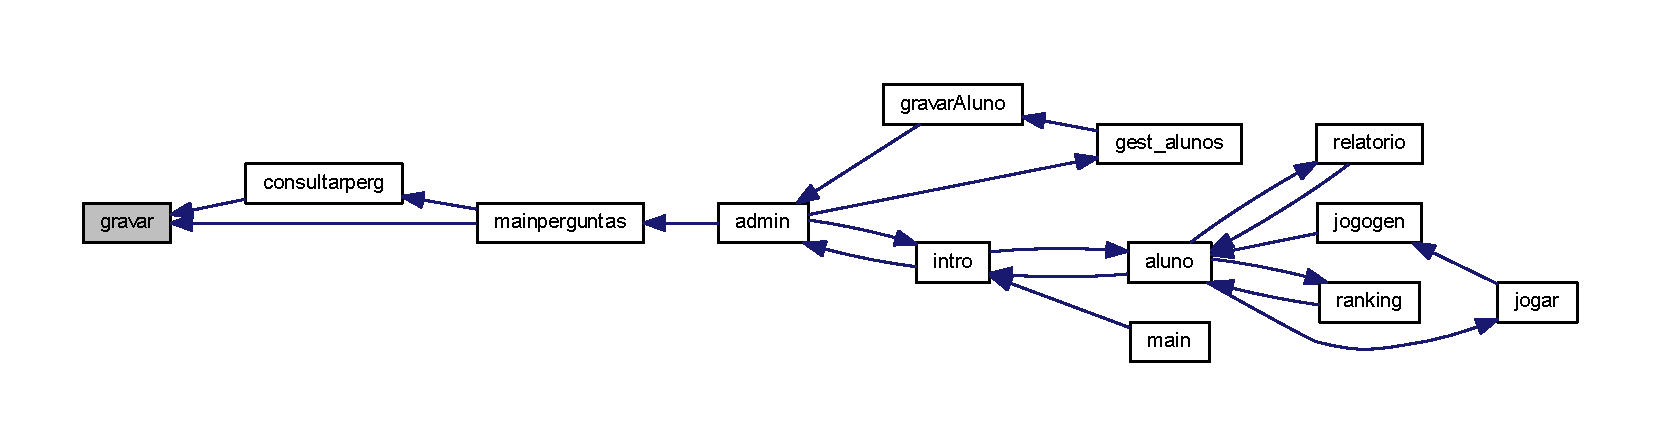
\includegraphics[width=350pt]{admin__perguntas_8h_a579492a6090f14af5ca1018dc507e3db_icgraph}
\end{center}
\end{figure}


\hypertarget{admin__perguntas_8h_a273151aa6319565d10bb075007dcc3a9}{\index{admin\+\_\+perguntas.\+h@{admin\+\_\+perguntas.\+h}!inserirperg@{inserirperg}}
\index{inserirperg@{inserirperg}!admin\+\_\+perguntas.\+h@{admin\+\_\+perguntas.\+h}}
\subsubsection[{inserirperg}]{\setlength{\rightskip}{0pt plus 5cm}void inserirperg (
\begin{DoxyParamCaption}
\item[{{\bf perguntas} $\ast$}]{x}
\end{DoxyParamCaption}
)}}\label{admin__perguntas_8h_a273151aa6319565d10bb075007dcc3a9}


funcao para inserir perguntas 

\textbackslash{} esta fun��o ir� permitir inserir novas perguntas \textbackslash{} recebe o parametro de entrada \char`\"{}perguntas\char`\"{}

Here is the caller graph for this function\+:\nopagebreak
\begin{figure}[H]
\begin{center}
\leavevmode
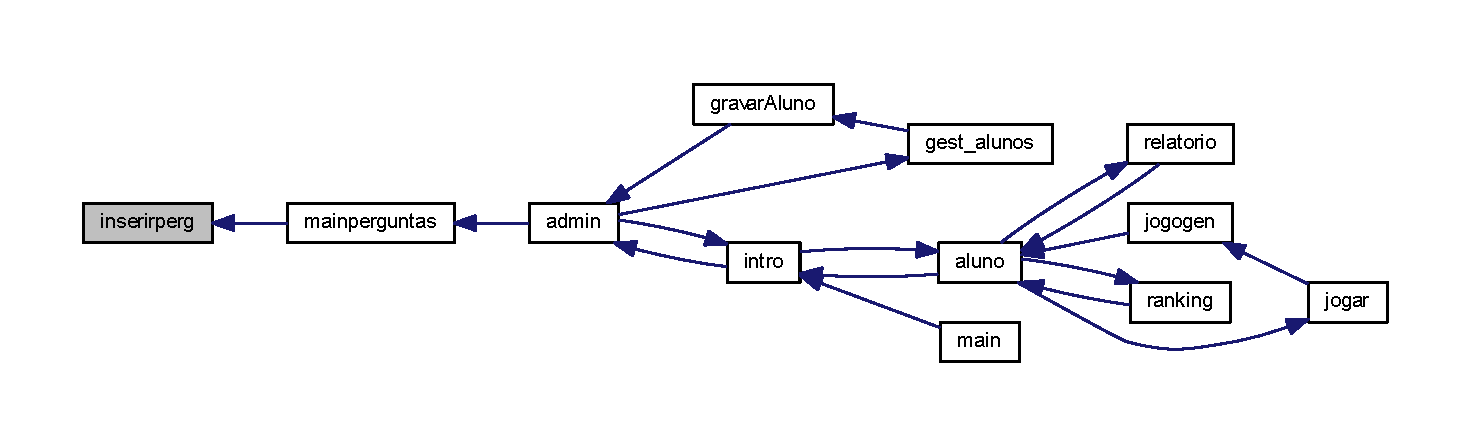
\includegraphics[width=350pt]{admin__perguntas_8h_a273151aa6319565d10bb075007dcc3a9_icgraph}
\end{center}
\end{figure}


\hypertarget{admin__perguntas_8h_a921c1f88176bd80774d8d1eaa3a80002}{\index{admin\+\_\+perguntas.\+h@{admin\+\_\+perguntas.\+h}!lerperguntas@{lerperguntas}}
\index{lerperguntas@{lerperguntas}!admin\+\_\+perguntas.\+h@{admin\+\_\+perguntas.\+h}}
\subsubsection[{lerperguntas}]{\setlength{\rightskip}{0pt plus 5cm}void lerperguntas (
\begin{DoxyParamCaption}
\item[{{\bf perguntas} $\ast$}]{x}
\end{DoxyParamCaption}
)}}\label{admin__perguntas_8h_a921c1f88176bd80774d8d1eaa3a80002}


funcao para ler o ficheiro de perguntas 

\textbackslash{} esta fun��o ir� permitir consultar o ficheiro existente perguntas.\+txt e carregar os dados existentes \textbackslash{} recebe o parametro de entrada \char`\"{}perguntas\char`\"{}

Here is the caller graph for this function\+:\nopagebreak
\begin{figure}[H]
\begin{center}
\leavevmode
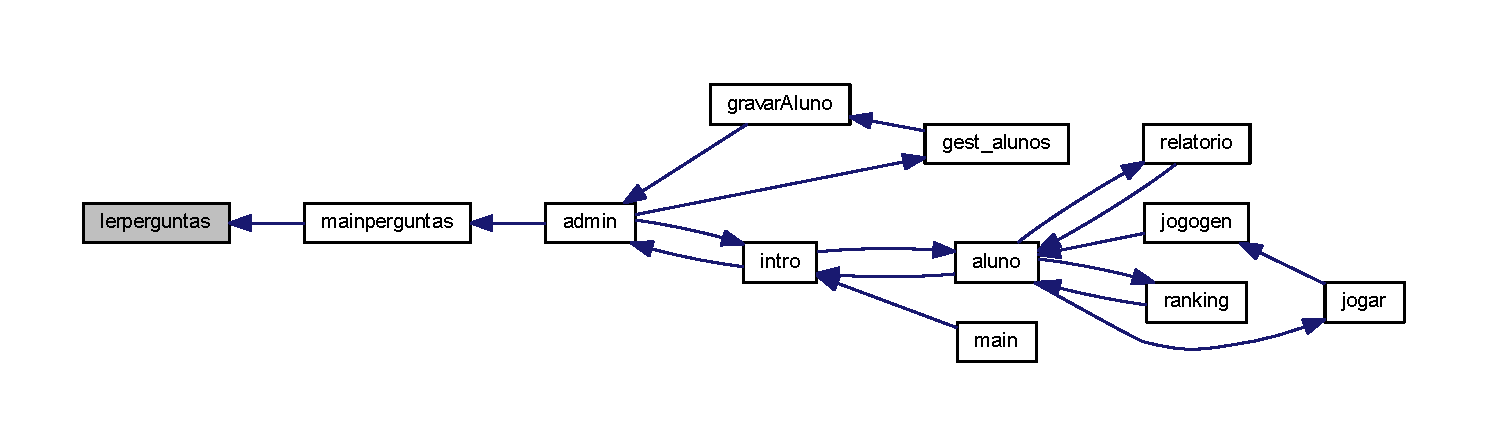
\includegraphics[width=350pt]{admin__perguntas_8h_a921c1f88176bd80774d8d1eaa3a80002_icgraph}
\end{center}
\end{figure}


\hypertarget{admin__perguntas_8h_a7ab3ce3466d990aa0d1f85a5d15a6716}{\index{admin\+\_\+perguntas.\+h@{admin\+\_\+perguntas.\+h}!mainperguntas@{mainperguntas}}
\index{mainperguntas@{mainperguntas}!admin\+\_\+perguntas.\+h@{admin\+\_\+perguntas.\+h}}
\subsubsection[{mainperguntas}]{\setlength{\rightskip}{0pt plus 5cm}mainperguntas (
\begin{DoxyParamCaption}
{}
\end{DoxyParamCaption}
)}}\label{admin__perguntas_8h_a7ab3ce3466d990aa0d1f85a5d15a6716}


Menu de Perguntas. 

fun��o do menu de perguntas 

Here is the call graph for this function\+:\nopagebreak
\begin{figure}[H]
\begin{center}
\leavevmode
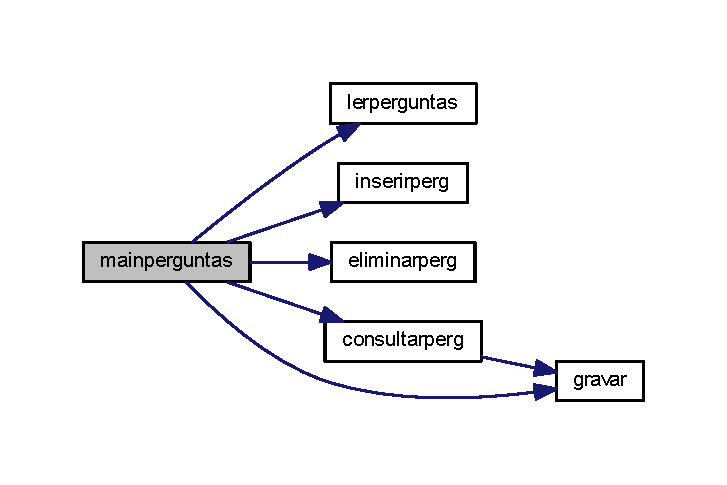
\includegraphics[width=349pt]{admin__perguntas_8h_a7ab3ce3466d990aa0d1f85a5d15a6716_cgraph}
\end{center}
\end{figure}




Here is the caller graph for this function\+:\nopagebreak
\begin{figure}[H]
\begin{center}
\leavevmode
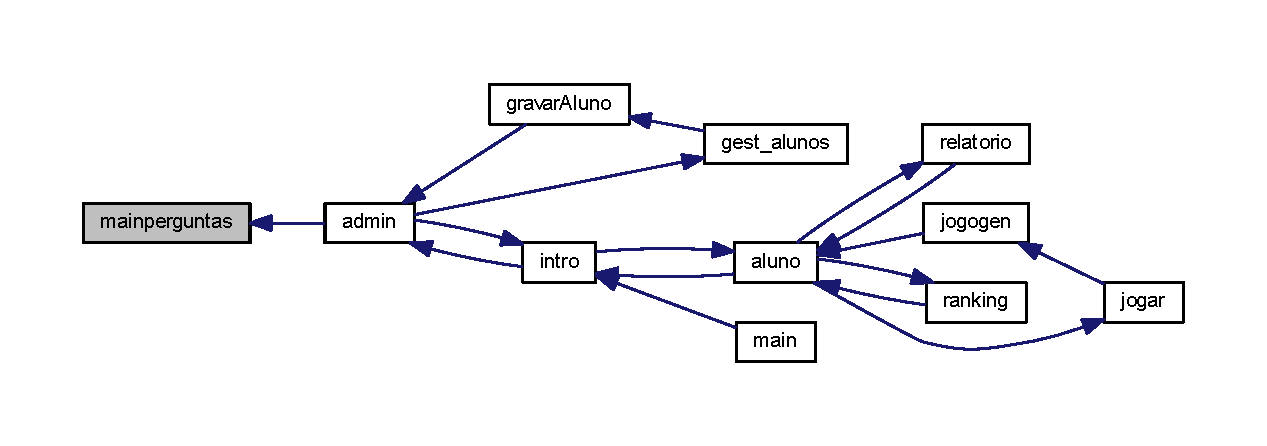
\includegraphics[width=350pt]{admin__perguntas_8h_a7ab3ce3466d990aa0d1f85a5d15a6716_icgraph}
\end{center}
\end{figure}



\hypertarget{estruturas_8h}{\section{C\+:/\+Users/manuelseromenho/\+Desktop/quizmaster3001/source/estruturas.h File Reference}
\label{estruturas_8h}\index{C\+:/\+Users/manuelseromenho/\+Desktop/quizmaster3001/source/estruturas.\+h@{C\+:/\+Users/manuelseromenho/\+Desktop/quizmaster3001/source/estruturas.\+h}}
}


ficheiro das estruturas do Quizmaster 3001  


This graph shows which files directly or indirectly include this file\+:\nopagebreak
\begin{figure}[H]
\begin{center}
\leavevmode
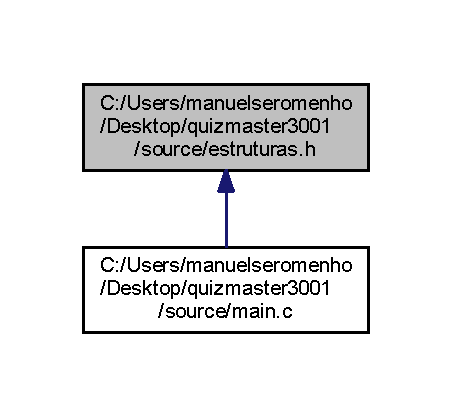
\includegraphics[width=217pt]{estruturas_8h__dep__incl}
\end{center}
\end{figure}
\subsection*{Data Structures}
\begin{DoxyCompactItemize}
\item 
struct \hyperlink{structperguntas}{perguntas}
\item 
struct \hyperlink{structperguntas__rand}{perguntas\+\_\+rand}
\item 
struct \hyperlink{structalunotab}{alunotab}
\end{DoxyCompactItemize}


\subsection{Detailed Description}
ficheiro das estruturas do Quizmaster 3001 

inclui os v�rios tipos de estrutura utilizado no Quizmaster 3001 \begin{DoxyAuthor}{Author}
Manuel Seromenho 
\end{DoxyAuthor}
\begin{DoxyDate}{Date}
14 Janeiro 2015 
\end{DoxyDate}
\begin{DoxyRefDesc}{Bug}
\item[\hyperlink{bug__bug000001}{Bug}]sem erros detetados \begin{DoxyWarning}{Warning}
nenhum warning 
\end{DoxyWarning}
\begin{DoxyVersion}{Version}
1.\+0 
\end{DoxyVersion}
\begin{DoxyCopyright}{Copyright}
G\+N\+U Public License. 
\end{DoxyCopyright}
\end{DoxyRefDesc}

\hypertarget{includes__defines_8h}{\section{C\+:/\+Users/manuelseromenho/\+Desktop/quizmaster3001/source/includes\+\_\+defines.h File Reference}
\label{includes__defines_8h}\index{C\+:/\+Users/manuelseromenho/\+Desktop/quizmaster3001/source/includes\+\_\+defines.\+h@{C\+:/\+Users/manuelseromenho/\+Desktop/quizmaster3001/source/includes\+\_\+defines.\+h}}
}


ficheiro dos includes e defines do Quizmaster 3001  


{\ttfamily \#include $<$stdio.\+h$>$}\\*
{\ttfamily \#include $<$stdlib.\+h$>$}\\*
{\ttfamily \#include $<$string.\+h$>$}\\*
{\ttfamily \#include $<$windows.\+h$>$}\\*
{\ttfamily \#include $<$time.\+h$>$}\\*
Include dependency graph for includes\+\_\+defines.\+h\+:\nopagebreak
\begin{figure}[H]
\begin{center}
\leavevmode
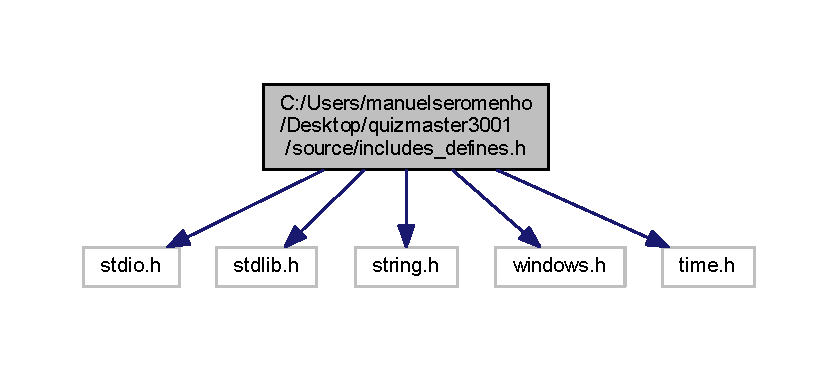
\includegraphics[width=350pt]{includes__defines_8h__incl}
\end{center}
\end{figure}
This graph shows which files directly or indirectly include this file\+:\nopagebreak
\begin{figure}[H]
\begin{center}
\leavevmode
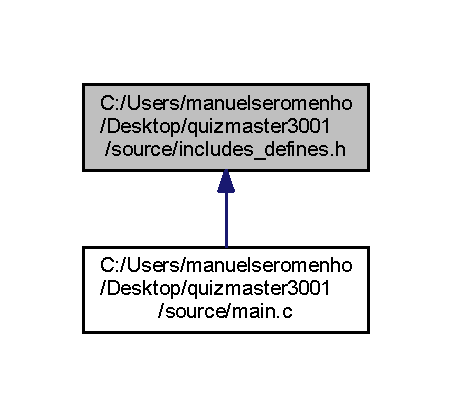
\includegraphics[width=217pt]{includes__defines_8h__dep__incl}
\end{center}
\end{figure}
\subsection*{Macros}
\begin{DoxyCompactItemize}
\item 
\#define \hyperlink{includes__defines_8h_af146485306ae74a2edf18636300fd107}{N\+R}~100
\item 
\#define \hyperlink{includes__defines_8h_ab04c88bedc6b2be8ddfe7aa8d3e93f06}{N\+P}~100
\item 
\#define \hyperlink{includes__defines_8h_ac16126e1e860a5541e593e483710fa4e}{S\+T\+R\+L\+N}~150
\item 
\#define \hyperlink{includes__defines_8h_adcc073d79edf75a1d9f0c31128b323b7}{N\+U\+M\+P\+E\+R\+\_\+\+R\+A\+N\+D}~10
\item 
\#define \hyperlink{includes__defines_8h_a68eddd535923d17ddbc8bb03bab70b3b}{N\+A}~100 /$\ast$$\ast$$\ast$$\ast$$\ast$/
\item 
\#define \hyperlink{includes__defines_8h_a58e95dc1eb9d6ce16f515e77beeadd58}{N\+B}~100 /$\ast$$\ast$$\ast$$\ast$$\ast$/
\end{DoxyCompactItemize}


\subsection{Detailed Description}
ficheiro dos includes e defines do Quizmaster 3001 

inclui os v�rios includes e defines prim�rios para o c�digo do Quizmaster 3001 \begin{DoxyAuthor}{Author}
Manuel Seromenho 
\end{DoxyAuthor}
\begin{DoxyDate}{Date}
14 Janeiro 2015 
\end{DoxyDate}
\begin{DoxyRefDesc}{Bug}
\item[\hyperlink{bug__bug000002}{Bug}]sem erros detetados \begin{DoxyWarning}{Warning}
nenhum warning 
\end{DoxyWarning}
\begin{DoxyVersion}{Version}
1.\+0 
\end{DoxyVersion}
\begin{DoxyCopyright}{Copyright}
G\+N\+U Public License. 
\end{DoxyCopyright}
\end{DoxyRefDesc}


\subsection{Macro Definition Documentation}
\hypertarget{includes__defines_8h_a68eddd535923d17ddbc8bb03bab70b3b}{\index{includes\+\_\+defines.\+h@{includes\+\_\+defines.\+h}!N\+A@{N\+A}}
\index{N\+A@{N\+A}!includes\+\_\+defines.\+h@{includes\+\_\+defines.\+h}}
\subsubsection[{N\+A}]{\setlength{\rightskip}{0pt plus 5cm}\#define N\+A~100 /$\ast$$\ast$$\ast$$\ast$$\ast$/}}\label{includes__defines_8h_a68eddd535923d17ddbc8bb03bab70b3b}
\hypertarget{includes__defines_8h_a58e95dc1eb9d6ce16f515e77beeadd58}{\index{includes\+\_\+defines.\+h@{includes\+\_\+defines.\+h}!N\+B@{N\+B}}
\index{N\+B@{N\+B}!includes\+\_\+defines.\+h@{includes\+\_\+defines.\+h}}
\subsubsection[{N\+B}]{\setlength{\rightskip}{0pt plus 5cm}\#define N\+B~100 /$\ast$$\ast$$\ast$$\ast$$\ast$/}}\label{includes__defines_8h_a58e95dc1eb9d6ce16f515e77beeadd58}
\hypertarget{includes__defines_8h_ab04c88bedc6b2be8ddfe7aa8d3e93f06}{\index{includes\+\_\+defines.\+h@{includes\+\_\+defines.\+h}!N\+P@{N\+P}}
\index{N\+P@{N\+P}!includes\+\_\+defines.\+h@{includes\+\_\+defines.\+h}}
\subsubsection[{N\+P}]{\setlength{\rightskip}{0pt plus 5cm}\#define N\+P~100}}\label{includes__defines_8h_ab04c88bedc6b2be8ddfe7aa8d3e93f06}
\hypertarget{includes__defines_8h_af146485306ae74a2edf18636300fd107}{\index{includes\+\_\+defines.\+h@{includes\+\_\+defines.\+h}!N\+R@{N\+R}}
\index{N\+R@{N\+R}!includes\+\_\+defines.\+h@{includes\+\_\+defines.\+h}}
\subsubsection[{N\+R}]{\setlength{\rightskip}{0pt plus 5cm}\#define N\+R~100}}\label{includes__defines_8h_af146485306ae74a2edf18636300fd107}
\hypertarget{includes__defines_8h_adcc073d79edf75a1d9f0c31128b323b7}{\index{includes\+\_\+defines.\+h@{includes\+\_\+defines.\+h}!N\+U\+M\+P\+E\+R\+\_\+\+R\+A\+N\+D@{N\+U\+M\+P\+E\+R\+\_\+\+R\+A\+N\+D}}
\index{N\+U\+M\+P\+E\+R\+\_\+\+R\+A\+N\+D@{N\+U\+M\+P\+E\+R\+\_\+\+R\+A\+N\+D}!includes\+\_\+defines.\+h@{includes\+\_\+defines.\+h}}
\subsubsection[{N\+U\+M\+P\+E\+R\+\_\+\+R\+A\+N\+D}]{\setlength{\rightskip}{0pt plus 5cm}\#define N\+U\+M\+P\+E\+R\+\_\+\+R\+A\+N\+D~10}}\label{includes__defines_8h_adcc073d79edf75a1d9f0c31128b323b7}
\hypertarget{includes__defines_8h_ac16126e1e860a5541e593e483710fa4e}{\index{includes\+\_\+defines.\+h@{includes\+\_\+defines.\+h}!S\+T\+R\+L\+N@{S\+T\+R\+L\+N}}
\index{S\+T\+R\+L\+N@{S\+T\+R\+L\+N}!includes\+\_\+defines.\+h@{includes\+\_\+defines.\+h}}
\subsubsection[{S\+T\+R\+L\+N}]{\setlength{\rightskip}{0pt plus 5cm}\#define S\+T\+R\+L\+N~150}}\label{includes__defines_8h_ac16126e1e860a5541e593e483710fa4e}

\hypertarget{jogogen_8h}{\section{C\+:/\+Users/manuelseromenho/\+Desktop/quizmaster3001/source/jogogen.h File Reference}
\label{jogogen_8h}\index{C\+:/\+Users/manuelseromenho/\+Desktop/quizmaster3001/source/jogogen.\+h@{C\+:/\+Users/manuelseromenho/\+Desktop/quizmaster3001/source/jogogen.\+h}}
}


ficheiro que trata do jogo gen�rico do Quizmaster 3001  


This graph shows which files directly or indirectly include this file\+:\nopagebreak
\begin{figure}[H]
\begin{center}
\leavevmode
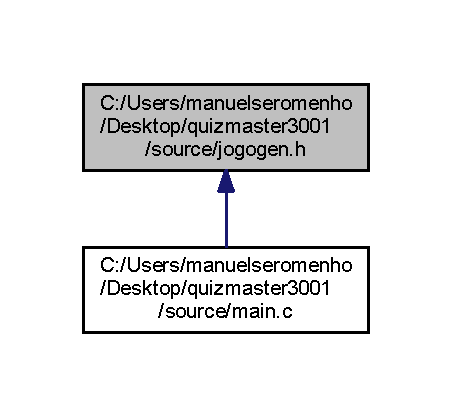
\includegraphics[width=217pt]{jogogen_8h__dep__incl}
\end{center}
\end{figure}
\subsection*{Functions}
\begin{DoxyCompactItemize}
\item 
void \hyperlink{jogogen_8h_af8fa28d8a123b8ae3b8d1a4201af5a02}{jogogen} (int iduser, \hyperlink{structperguntas__rand}{perguntas\+\_\+rand} $\ast$rand\+\_\+x, \hyperlink{structalunotab}{alunotab} $\ast$alu, int indice)
\begin{DoxyCompactList}\small\item\em funcao do jogo \end{DoxyCompactList}\item 
void \hyperlink{jogogen_8h_a9d5959cb84d9c4595414777c8b369a63}{ranking} (int iduser, \hyperlink{structalunotab}{alunotab} $\ast$alu)
\begin{DoxyCompactList}\small\item\em ranking dos jogadores(users/alunos) \end{DoxyCompactList}\item 
void \hyperlink{jogogen_8h_ae7b00fddd3e91259825cc51f1245bee9}{jogar} (int iduser, \hyperlink{structalunotab}{alunotab} $\ast$alu, char $\ast$nome, int indice)
\begin{DoxyCompactList}\small\item\em Menu Jogar. \end{DoxyCompactList}\item 
void \hyperlink{jogogen_8h_aa5261eb183e95885ae792f8ff46e3e53}{relatorio} (int iduser, \hyperlink{structalunotab}{alunotab} $\ast$alu, char $\ast$nome, int indice)
\begin{DoxyCompactList}\small\item\em Relatorio. \end{DoxyCompactList}\item 
void \hyperlink{jogogen_8h_a70c17e7e0c772226a81cccf10ff14a87}{aluno} (int iduser, \hyperlink{structalunotab}{alunotab} $\ast$alu)
\begin{DoxyCompactList}\small\item\em Menu aluno/user. \end{DoxyCompactList}\item 
void \hyperlink{jogogen_8h_a0fec8b8a1101b6da82a9a791de123d4d}{classi} (int rerrada, char out\mbox{[}30\mbox{]})
\begin{DoxyCompactList}\small\item\em Classificacao. \end{DoxyCompactList}\end{DoxyCompactItemize}


\subsection{Detailed Description}
ficheiro que trata do jogo gen�rico do Quizmaster 3001 

Esta parte do c�digo executa o jogo, utilizando toda a informa��o armazenada nos ficheiros \char`\"{}users.\+txt\char`\"{} e \char`\"{}perguntas.\+txt\char`\"{} \begin{DoxyAuthor}{Author}
Manuel Seromenho 
\end{DoxyAuthor}
\begin{DoxyDate}{Date}
17 Janeiro 2015 
\end{DoxyDate}
\begin{DoxyRefDesc}{Bug}
\item[\hyperlink{bug__bug000003}{Bug}]sem erros detetados \begin{DoxyWarning}{Warning}
nenhum warning 
\end{DoxyWarning}
\begin{DoxyVersion}{Version}
1.\+0 
\end{DoxyVersion}
\begin{DoxyCopyright}{Copyright}
G\+N\+U Public License. 
\end{DoxyCopyright}
\end{DoxyRefDesc}


\subsection{Function Documentation}
\hypertarget{jogogen_8h_a70c17e7e0c772226a81cccf10ff14a87}{\index{jogogen.\+h@{jogogen.\+h}!aluno@{aluno}}
\index{aluno@{aluno}!jogogen.\+h@{jogogen.\+h}}
\subsubsection[{aluno}]{\setlength{\rightskip}{0pt plus 5cm}void aluno (
\begin{DoxyParamCaption}
\item[{int}]{iduser, }
\item[{{\bf alunotab} $\ast$}]{alu}
\end{DoxyParamCaption}
)}}\label{jogogen_8h_a70c17e7e0c772226a81cccf10ff14a87}


Menu aluno/user. 

funcao menu aluno 
\begin{DoxyParams}{Parameters}
{\em iduser} & \+: int \\
\hline
{\em $\ast$alu} & \+: alunotab \\
\hline
\end{DoxyParams}
\begin{DoxyReturn}{Returns}
void 
\end{DoxyReturn}


Here is the call graph for this function\+:\nopagebreak
\begin{figure}[H]
\begin{center}
\leavevmode
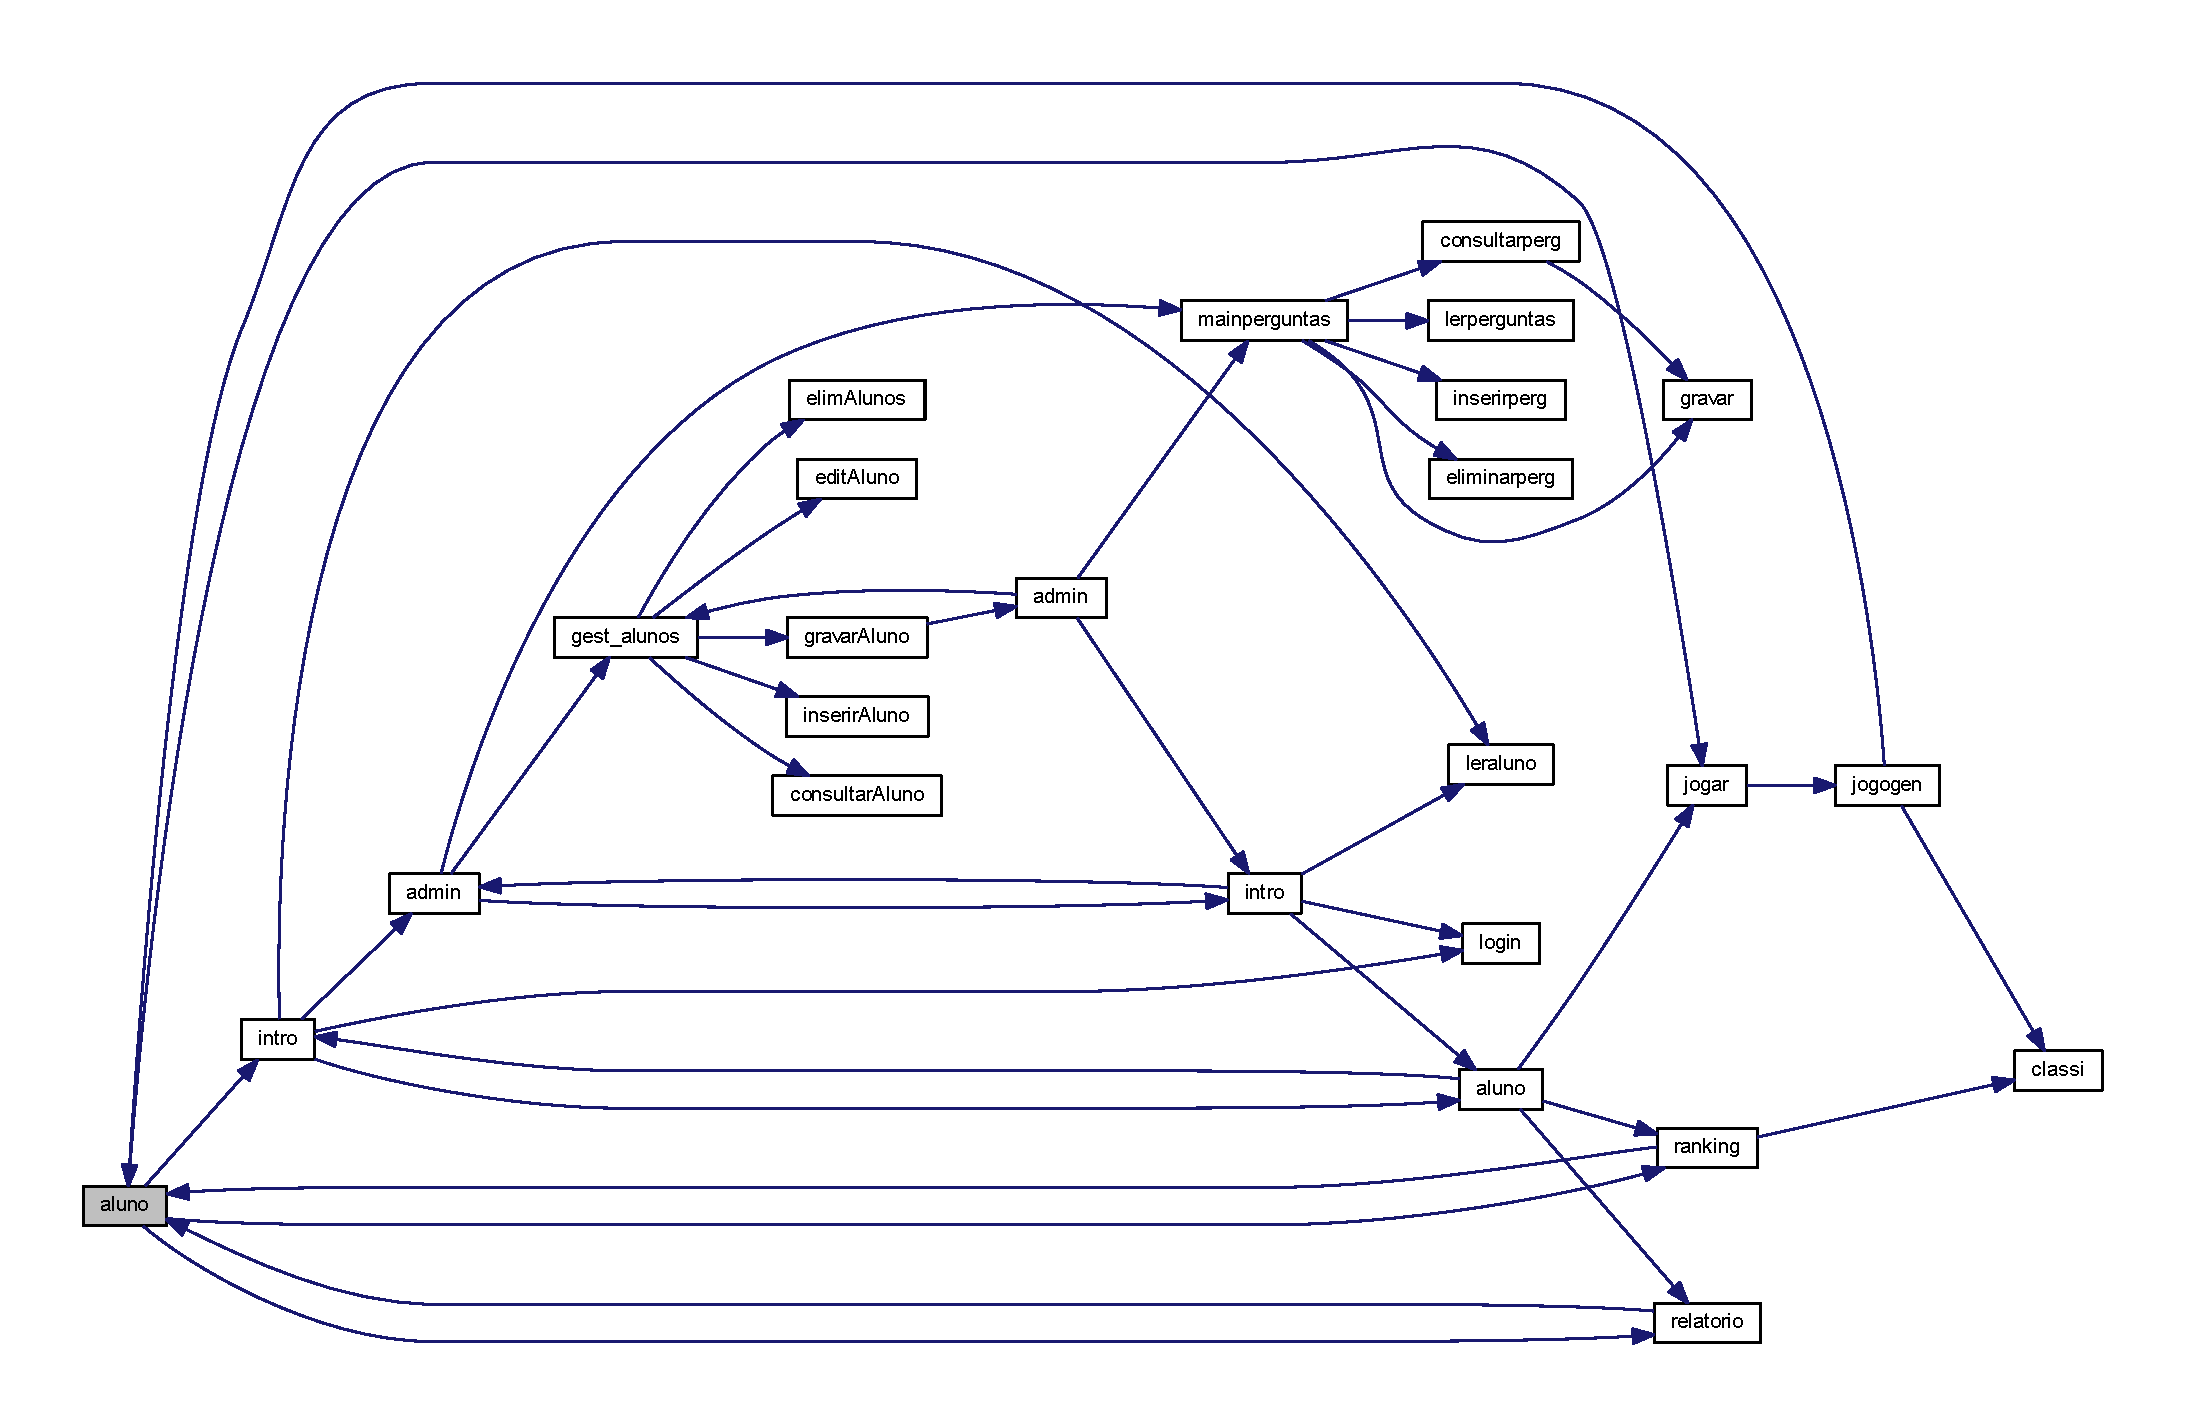
\includegraphics[width=350pt]{jogogen_8h_a70c17e7e0c772226a81cccf10ff14a87_cgraph}
\end{center}
\end{figure}




Here is the caller graph for this function\+:\nopagebreak
\begin{figure}[H]
\begin{center}
\leavevmode
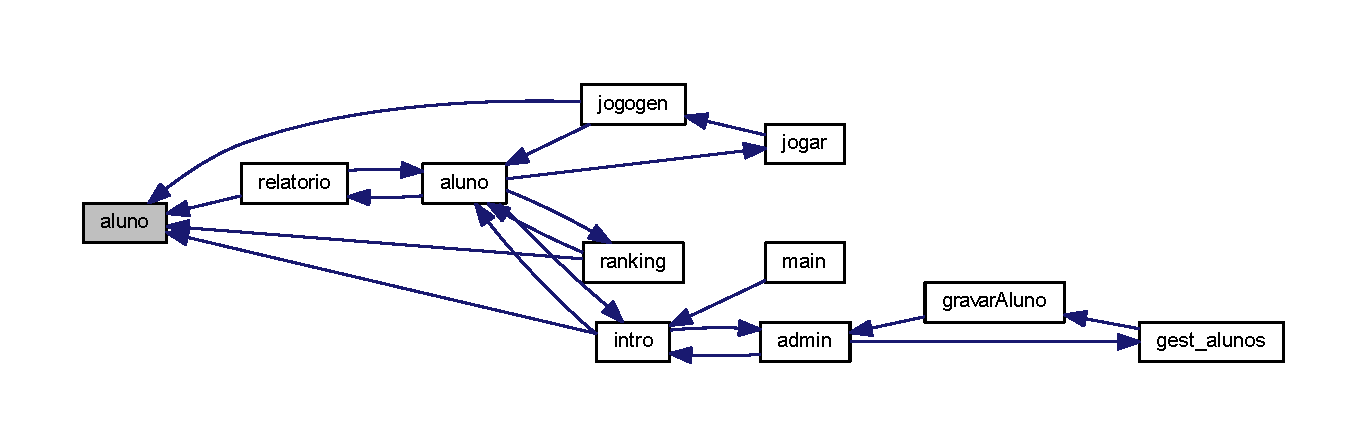
\includegraphics[width=350pt]{jogogen_8h_a70c17e7e0c772226a81cccf10ff14a87_icgraph}
\end{center}
\end{figure}


\hypertarget{jogogen_8h_a0fec8b8a1101b6da82a9a791de123d4d}{\index{jogogen.\+h@{jogogen.\+h}!classi@{classi}}
\index{classi@{classi}!jogogen.\+h@{jogogen.\+h}}
\subsubsection[{classi}]{\setlength{\rightskip}{0pt plus 5cm}void classi (
\begin{DoxyParamCaption}
\item[{int}]{rerrada, }
\item[{char}]{out\mbox{[}30\mbox{]}}
\end{DoxyParamCaption}
)}}\label{jogogen_8h_a0fec8b8a1101b6da82a9a791de123d4d}


Classificacao. 

funcao que determina a classica��o do jogador 
\begin{DoxyParams}{Parameters}
{\em rerrada} & \+: float \\
\hline
{\em out\mbox{[}$\,$\mbox{]}} & \+: char \\
\hline
\end{DoxyParams}
\begin{DoxyReturn}{Returns}
void 
\end{DoxyReturn}


Here is the caller graph for this function\+:\nopagebreak
\begin{figure}[H]
\begin{center}
\leavevmode
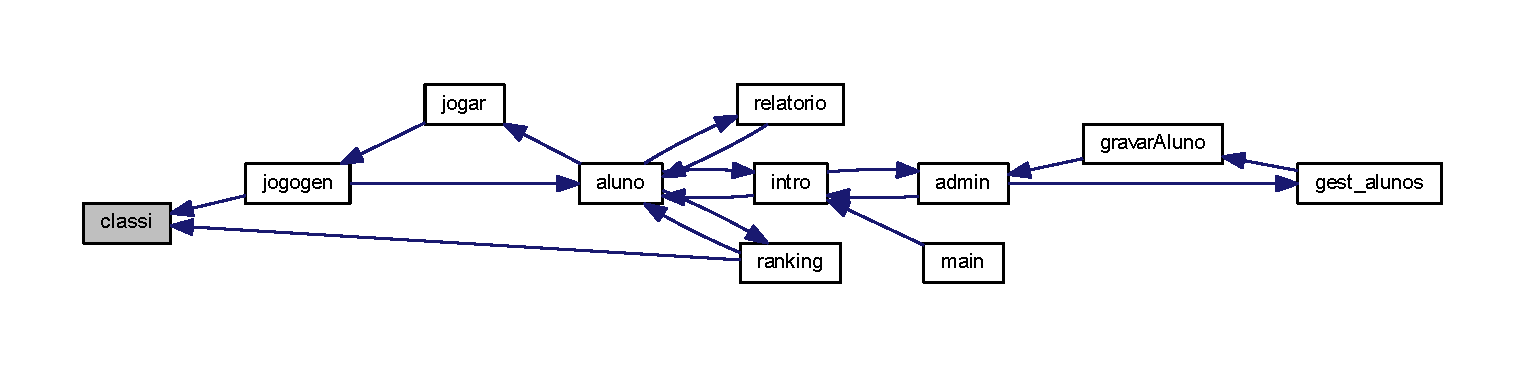
\includegraphics[width=350pt]{jogogen_8h_a0fec8b8a1101b6da82a9a791de123d4d_icgraph}
\end{center}
\end{figure}


\hypertarget{jogogen_8h_ae7b00fddd3e91259825cc51f1245bee9}{\index{jogogen.\+h@{jogogen.\+h}!jogar@{jogar}}
\index{jogar@{jogar}!jogogen.\+h@{jogogen.\+h}}
\subsubsection[{jogar}]{\setlength{\rightskip}{0pt plus 5cm}void jogar (
\begin{DoxyParamCaption}
\item[{int}]{iduser, }
\item[{{\bf alunotab} $\ast$}]{alu, }
\item[{char $\ast$}]{nome, }
\item[{int}]{indice}
\end{DoxyParamCaption}
)}}\label{jogogen_8h_ae7b00fddd3e91259825cc51f1245bee9}


Menu Jogar. 

funcao inicio do jogo (caso seja necess�rio futuramente ser� possivel escolher outros modos de jogo para al�m do gen�rico) 
\begin{DoxyParams}{Parameters}
{\em iduser} & \+: int \\
\hline
{\em $\ast$alu} & \+: alunotab \\
\hline
{\em nome} & \+: $\ast$char \\
\hline
{\em indice} & \+: indice \\
\hline
\end{DoxyParams}
\begin{DoxyReturn}{Returns}
void 
\end{DoxyReturn}


Here is the call graph for this function\+:\nopagebreak
\begin{figure}[H]
\begin{center}
\leavevmode
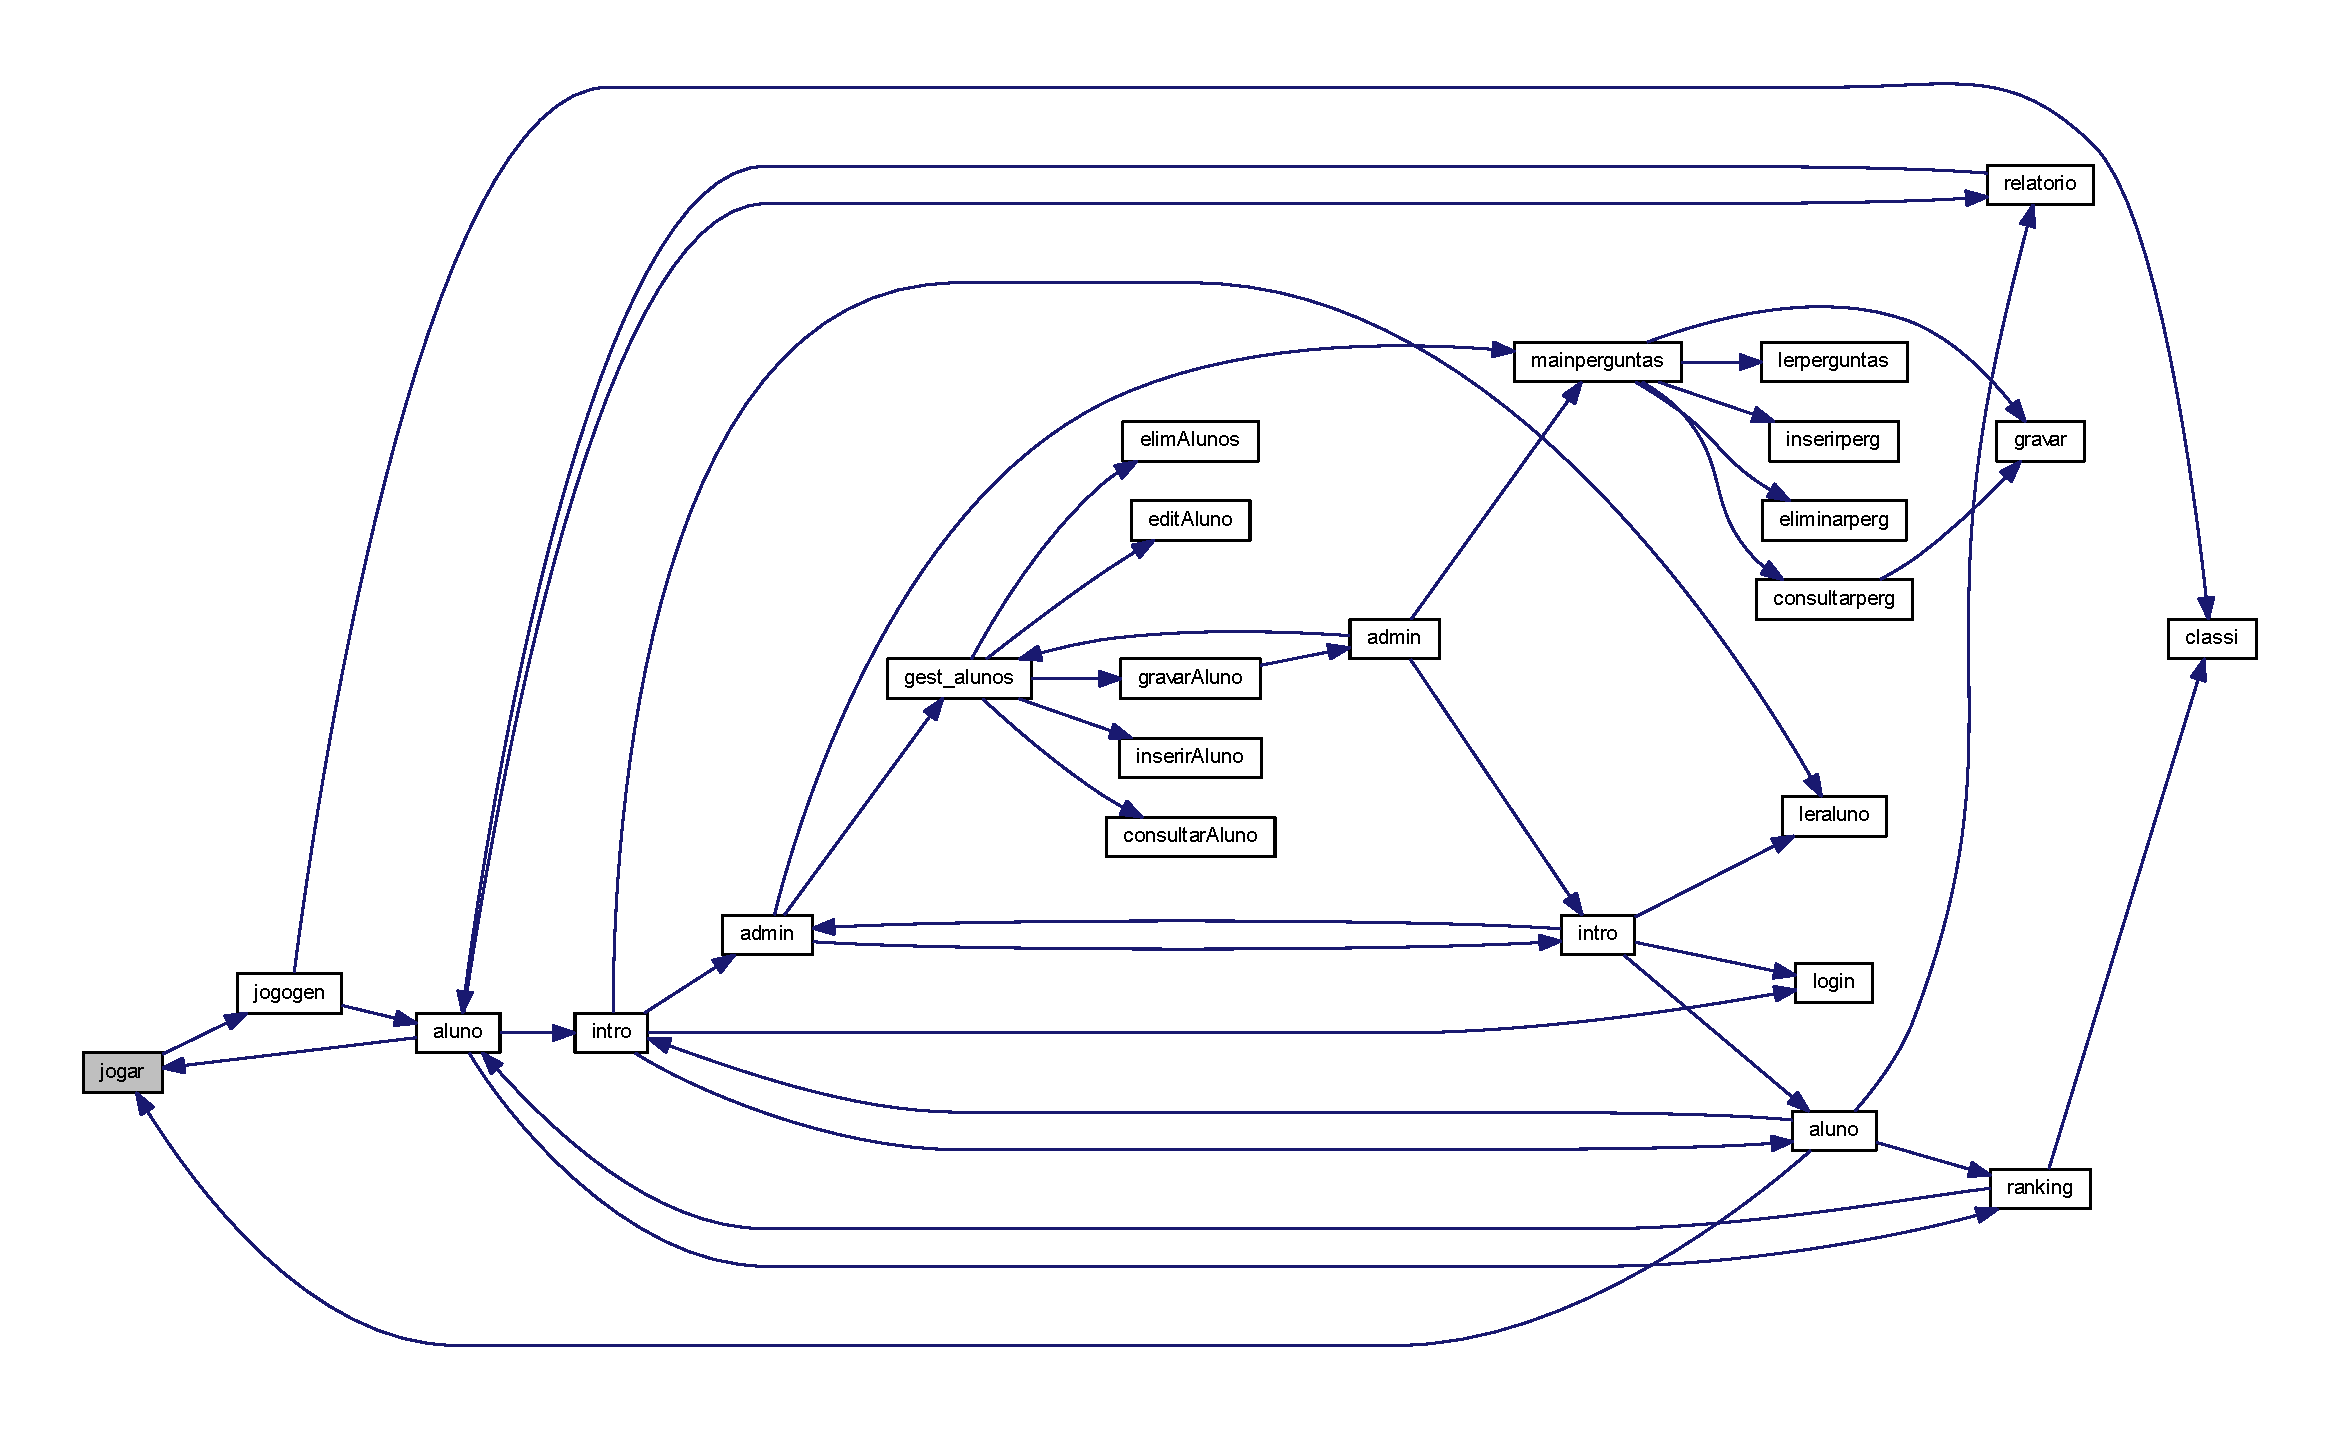
\includegraphics[width=350pt]{jogogen_8h_ae7b00fddd3e91259825cc51f1245bee9_cgraph}
\end{center}
\end{figure}




Here is the caller graph for this function\+:\nopagebreak
\begin{figure}[H]
\begin{center}
\leavevmode
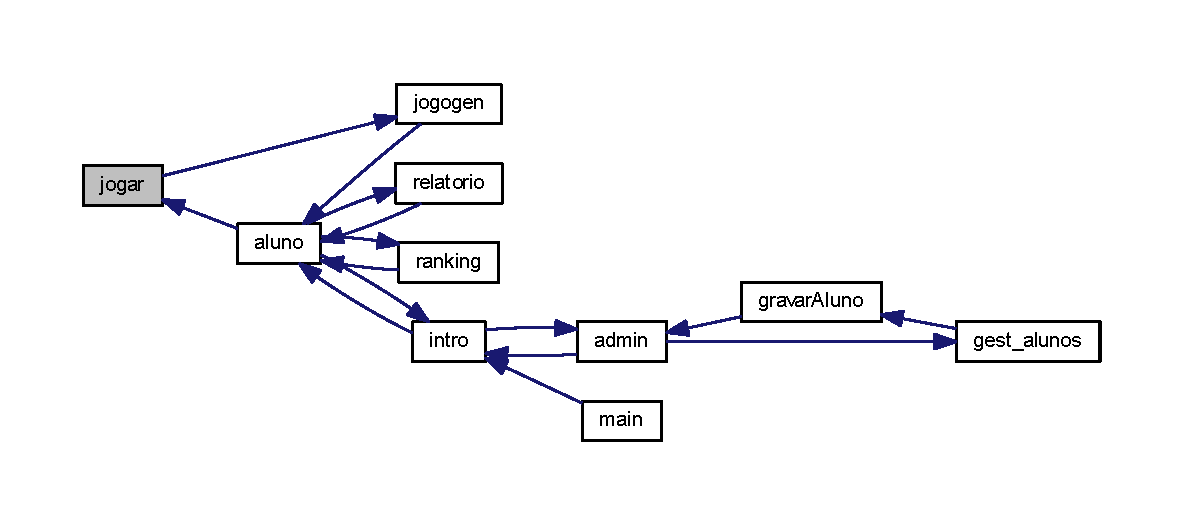
\includegraphics[width=350pt]{jogogen_8h_ae7b00fddd3e91259825cc51f1245bee9_icgraph}
\end{center}
\end{figure}


\hypertarget{jogogen_8h_af8fa28d8a123b8ae3b8d1a4201af5a02}{\index{jogogen.\+h@{jogogen.\+h}!jogogen@{jogogen}}
\index{jogogen@{jogogen}!jogogen.\+h@{jogogen.\+h}}
\subsubsection[{jogogen}]{\setlength{\rightskip}{0pt plus 5cm}void jogogen (
\begin{DoxyParamCaption}
\item[{int}]{iduser, }
\item[{{\bf perguntas\+\_\+rand} $\ast$}]{rand\+\_\+x, }
\item[{{\bf alunotab} $\ast$}]{alu, }
\item[{int}]{indice}
\end{DoxyParamCaption}
)}}\label{jogogen_8h_af8fa28d8a123b8ae3b8d1a4201af5a02}


funcao do jogo 

funcao do jogo (esta funcao executa o jogo em si) 
\begin{DoxyParams}{Parameters}
{\em iduser} & \+: int \\
\hline
{\em $\ast$rand\+\_\+x} & \+: \hyperlink{structperguntas__rand}{perguntas\+\_\+rand} \\
\hline
{\em $\ast$alu} & \+: alunotab \\
\hline
{\em indice} & \+: indice \\
\hline
\end{DoxyParams}
\begin{DoxyReturn}{Returns}
void 
\end{DoxyReturn}


Here is the call graph for this function\+:\nopagebreak
\begin{figure}[H]
\begin{center}
\leavevmode
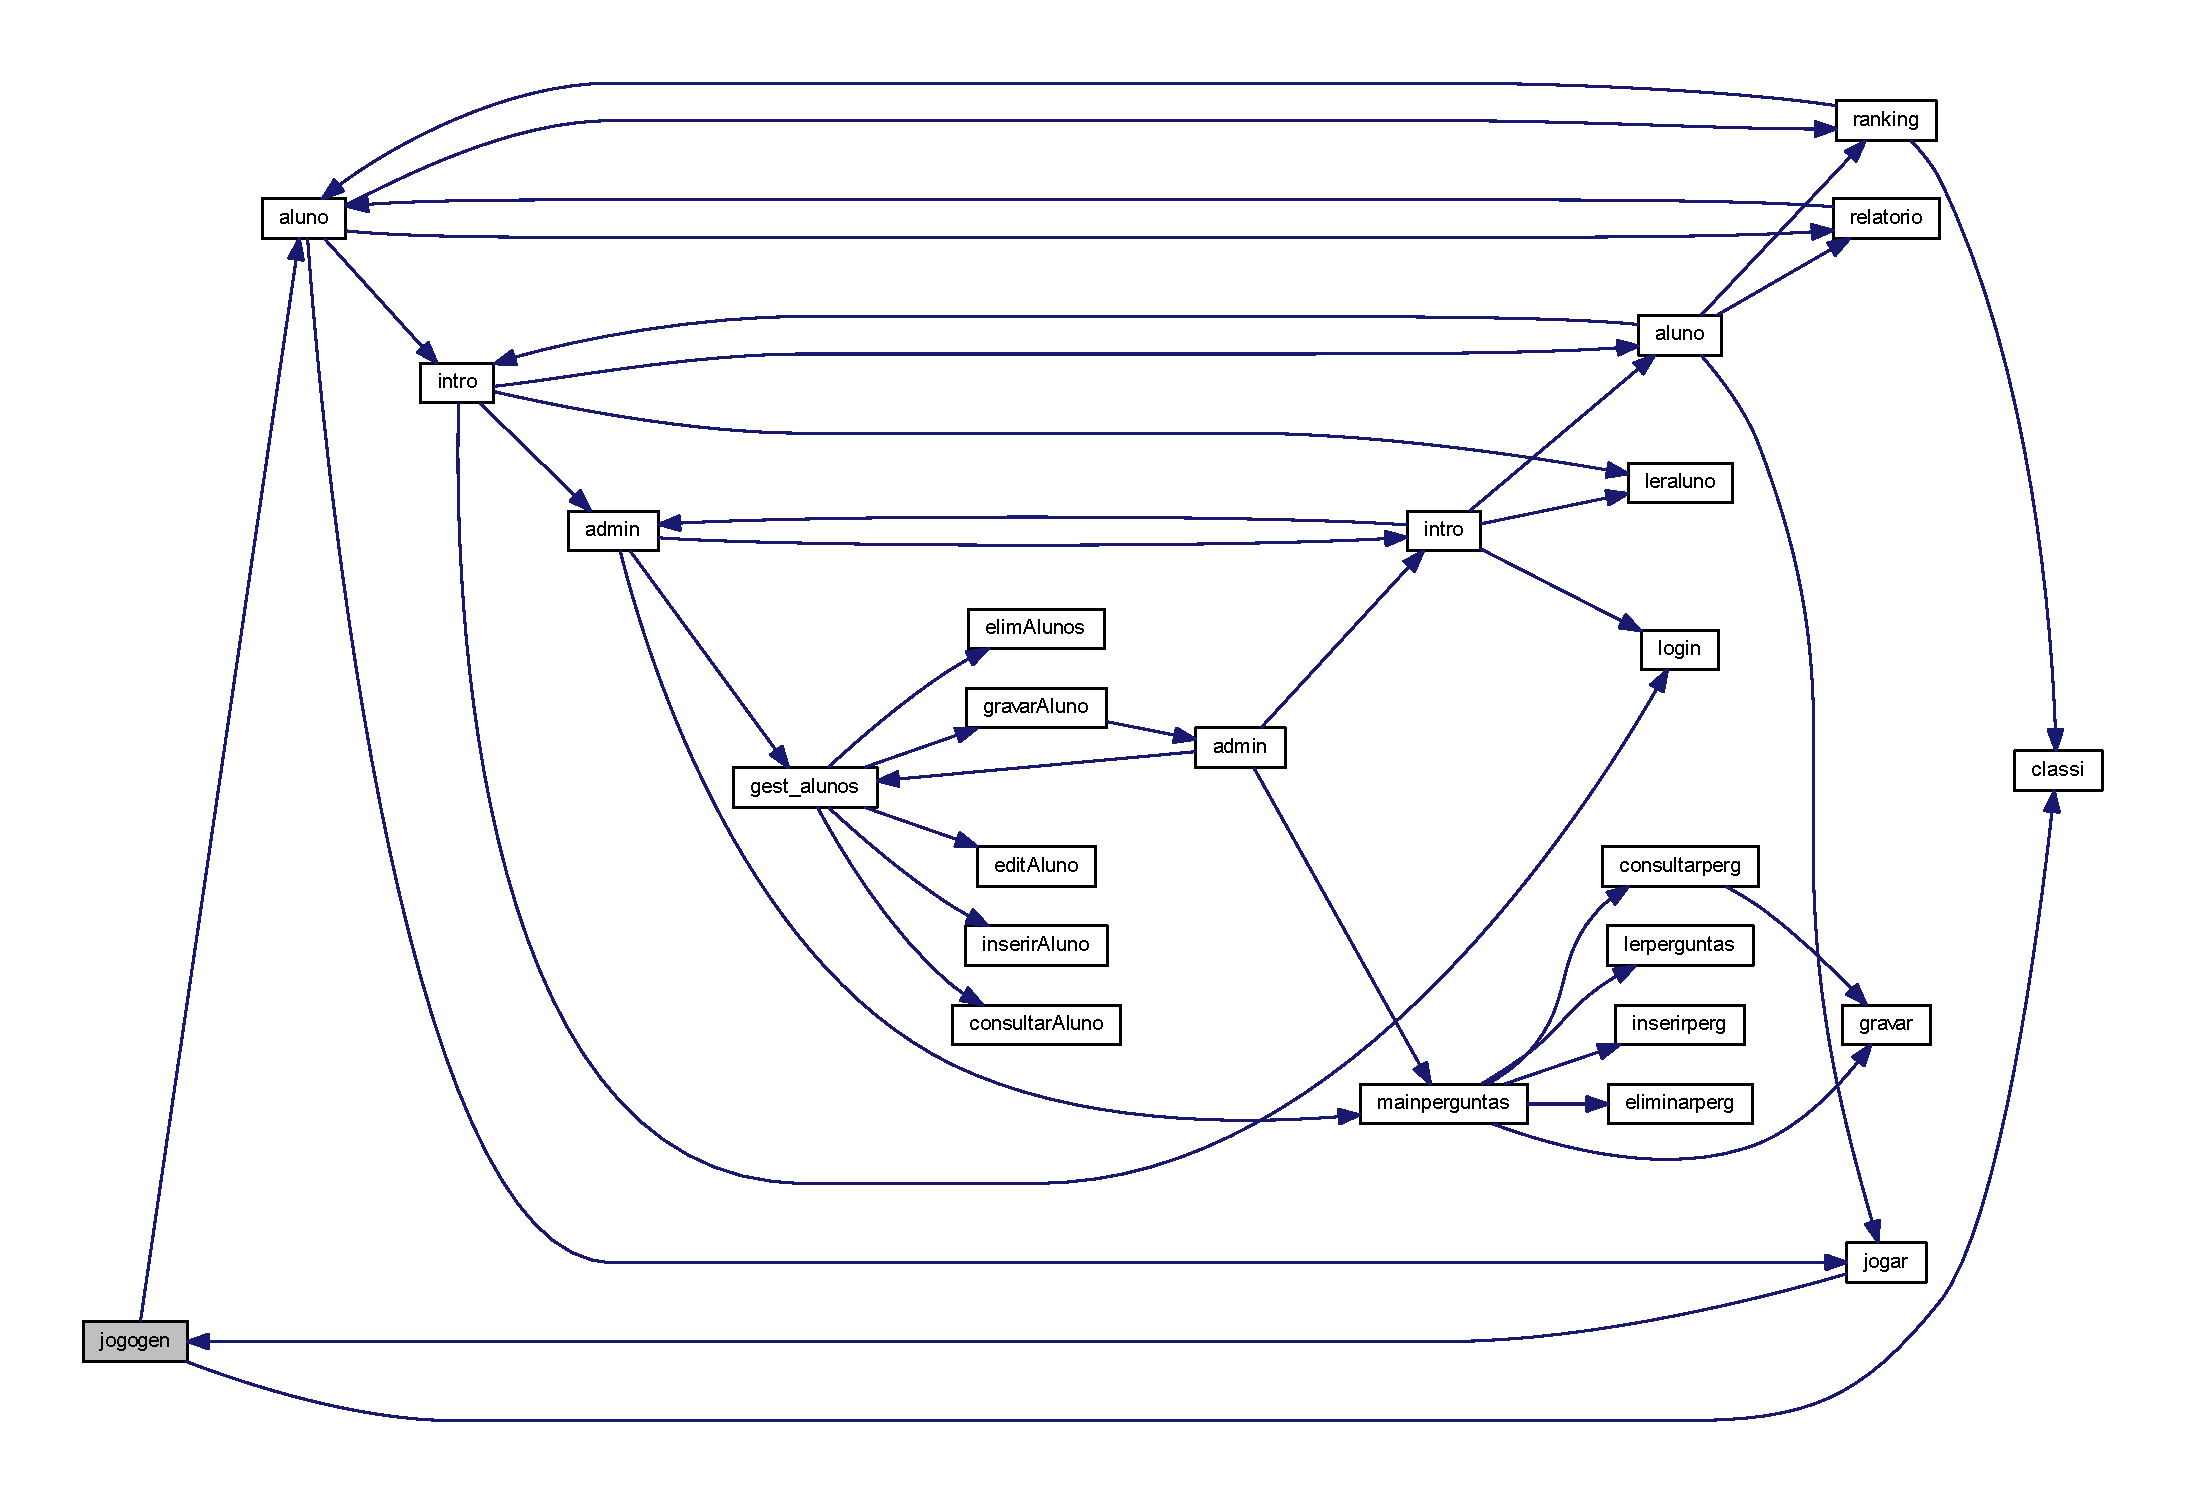
\includegraphics[width=350pt]{jogogen_8h_af8fa28d8a123b8ae3b8d1a4201af5a02_cgraph}
\end{center}
\end{figure}




Here is the caller graph for this function\+:\nopagebreak
\begin{figure}[H]
\begin{center}
\leavevmode
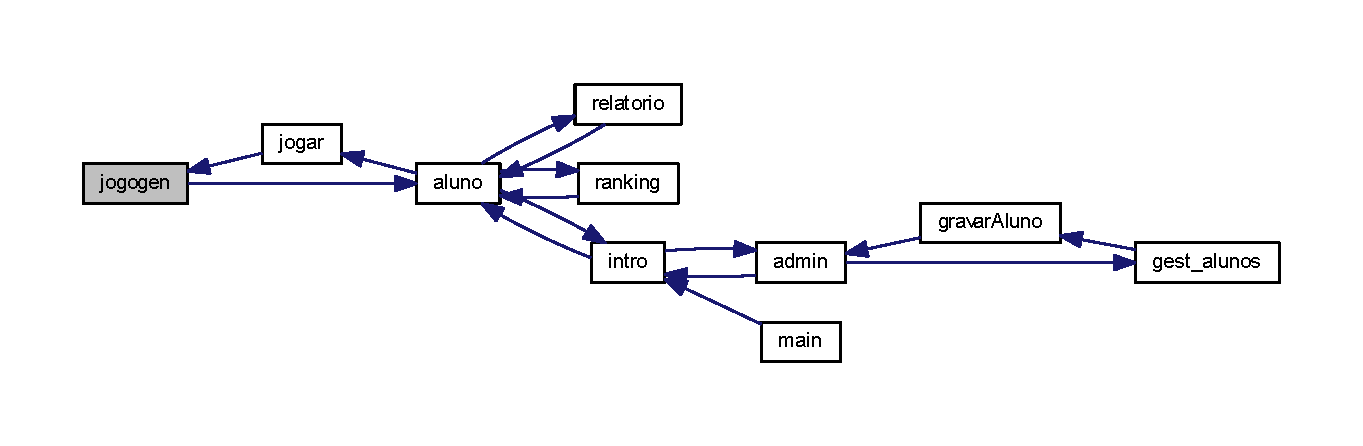
\includegraphics[width=350pt]{jogogen_8h_af8fa28d8a123b8ae3b8d1a4201af5a02_icgraph}
\end{center}
\end{figure}


\hypertarget{jogogen_8h_a9d5959cb84d9c4595414777c8b369a63}{\index{jogogen.\+h@{jogogen.\+h}!ranking@{ranking}}
\index{ranking@{ranking}!jogogen.\+h@{jogogen.\+h}}
\subsubsection[{ranking}]{\setlength{\rightskip}{0pt plus 5cm}void ranking (
\begin{DoxyParamCaption}
\item[{int}]{iduser, }
\item[{{\bf alunotab} $\ast$}]{alu}
\end{DoxyParamCaption}
)}}\label{jogogen_8h_a9d5959cb84d9c4595414777c8b369a63}


ranking dos jogadores(users/alunos) 

funcao ranking, analisa a pontua��o de casa jogador e lista ordenadamente 
\begin{DoxyParams}{Parameters}
{\em iduser} & \+: int \\
\hline
{\em $\ast$alu} & \+: alunotab \\
\hline
\end{DoxyParams}
\begin{DoxyReturn}{Returns}
void 
\end{DoxyReturn}


Here is the call graph for this function\+:\nopagebreak
\begin{figure}[H]
\begin{center}
\leavevmode
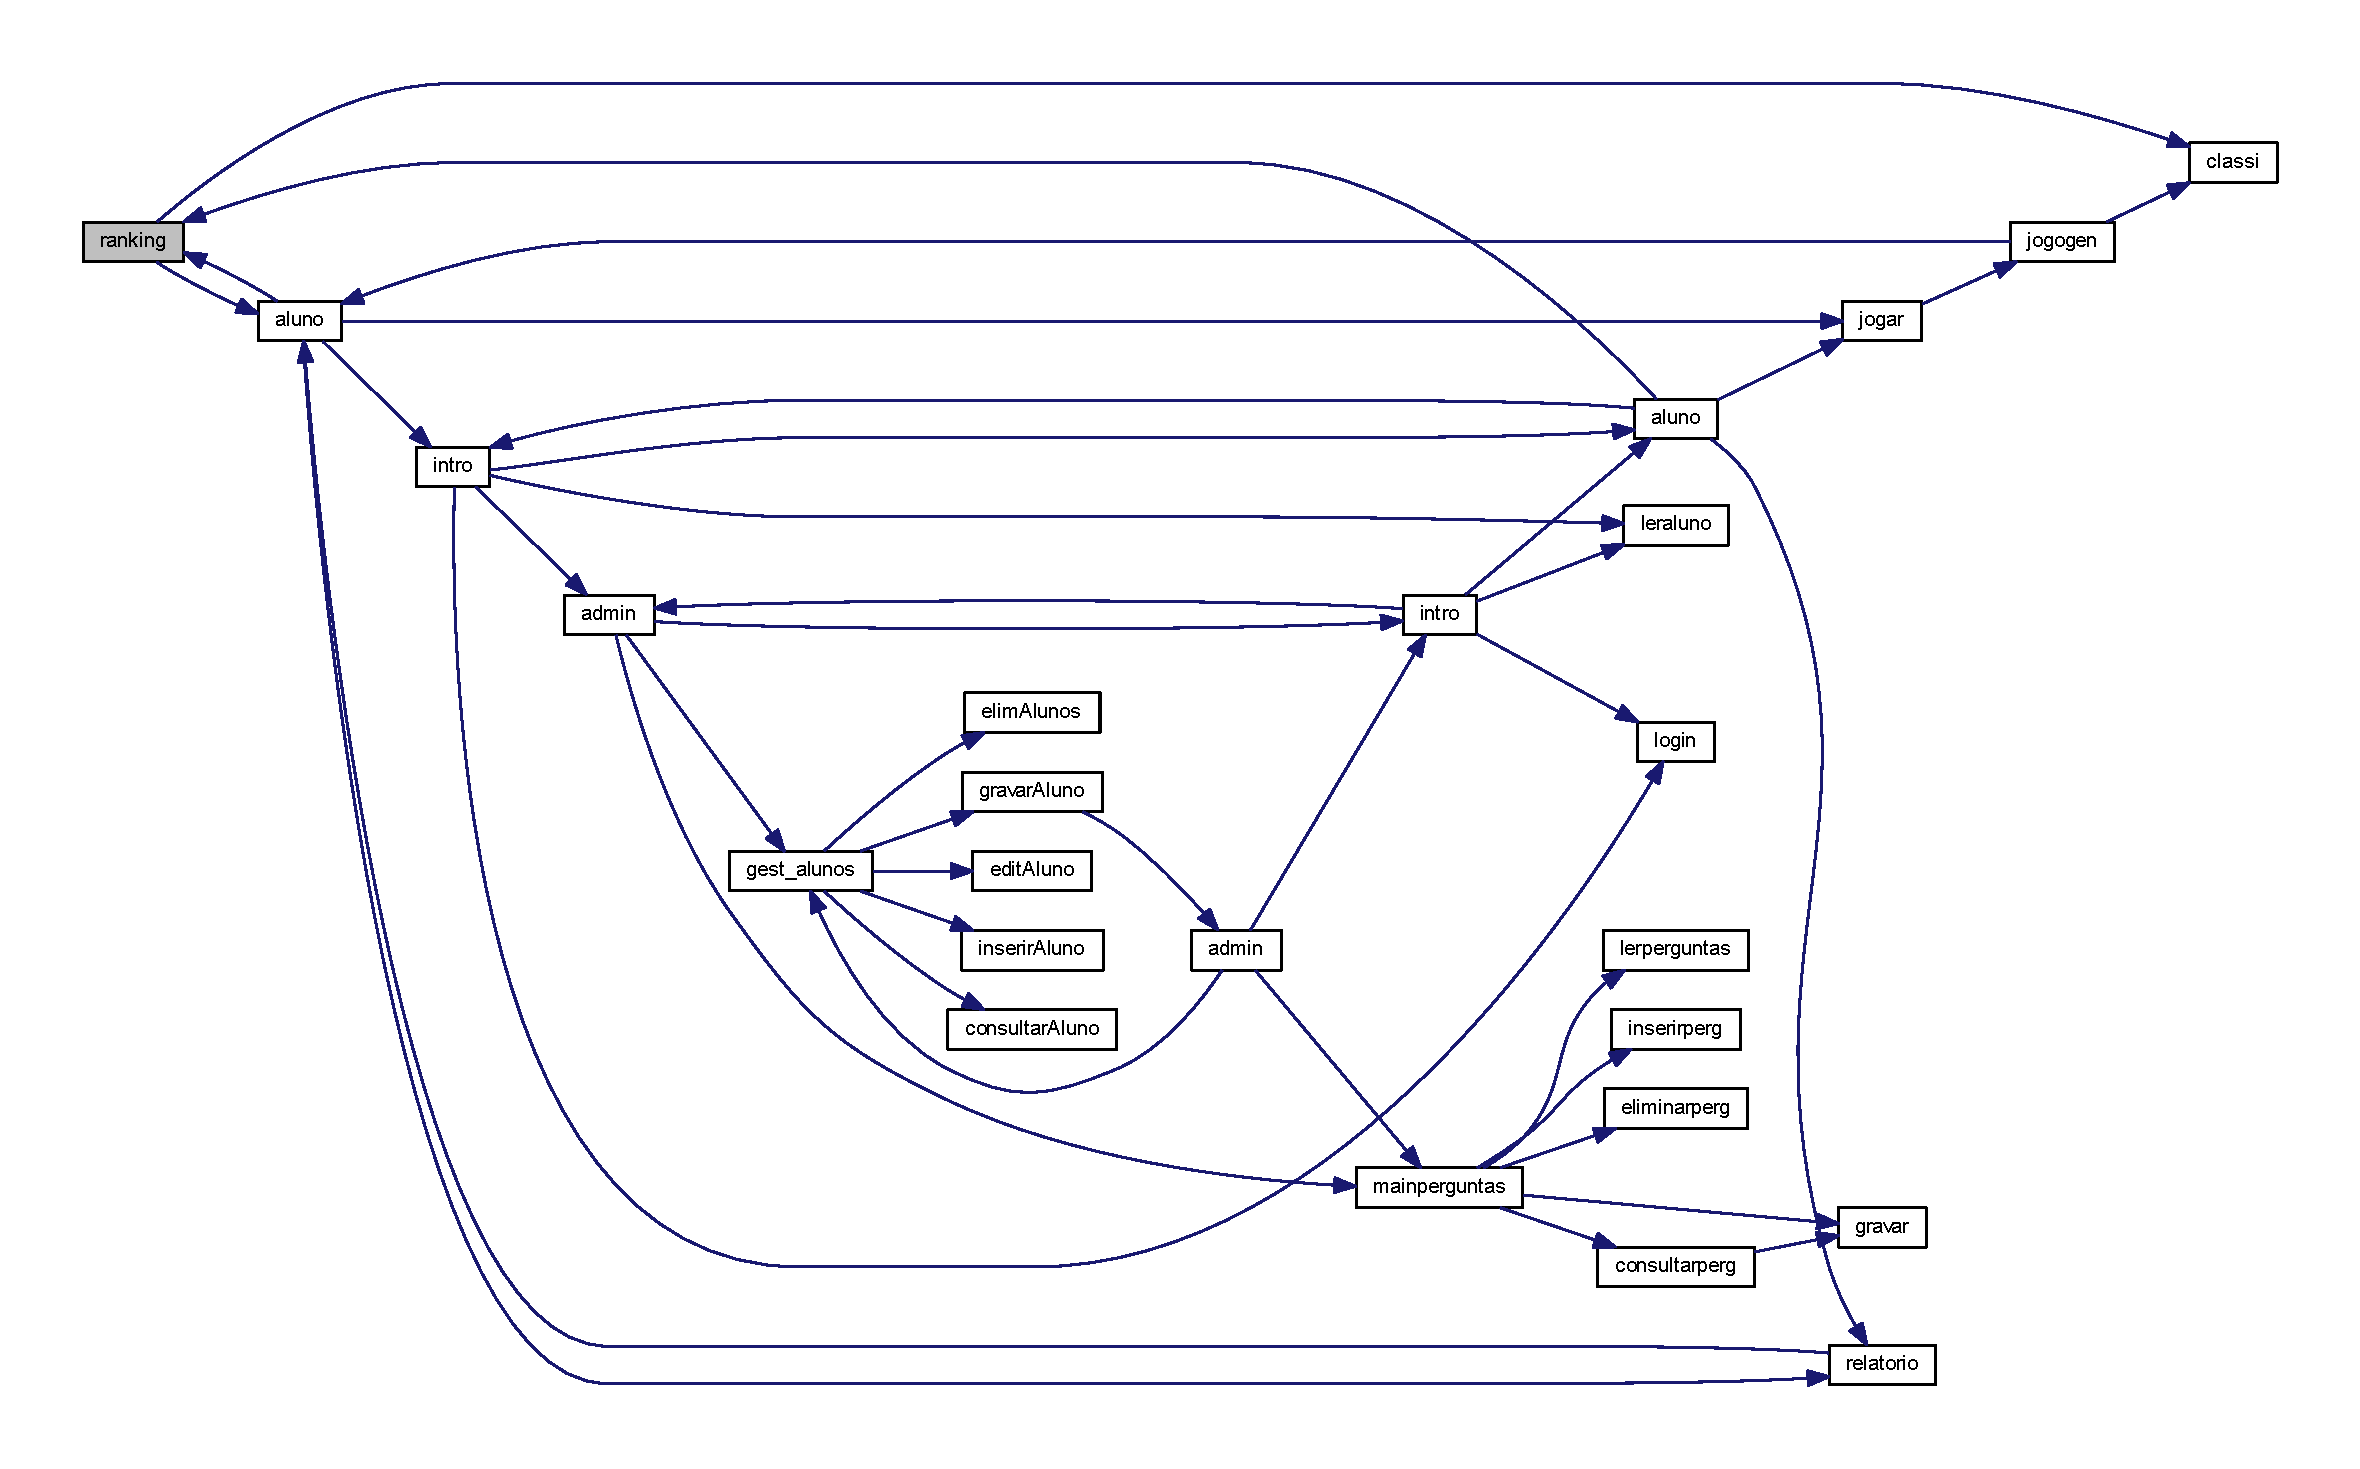
\includegraphics[width=350pt]{jogogen_8h_a9d5959cb84d9c4595414777c8b369a63_cgraph}
\end{center}
\end{figure}




Here is the caller graph for this function\+:\nopagebreak
\begin{figure}[H]
\begin{center}
\leavevmode
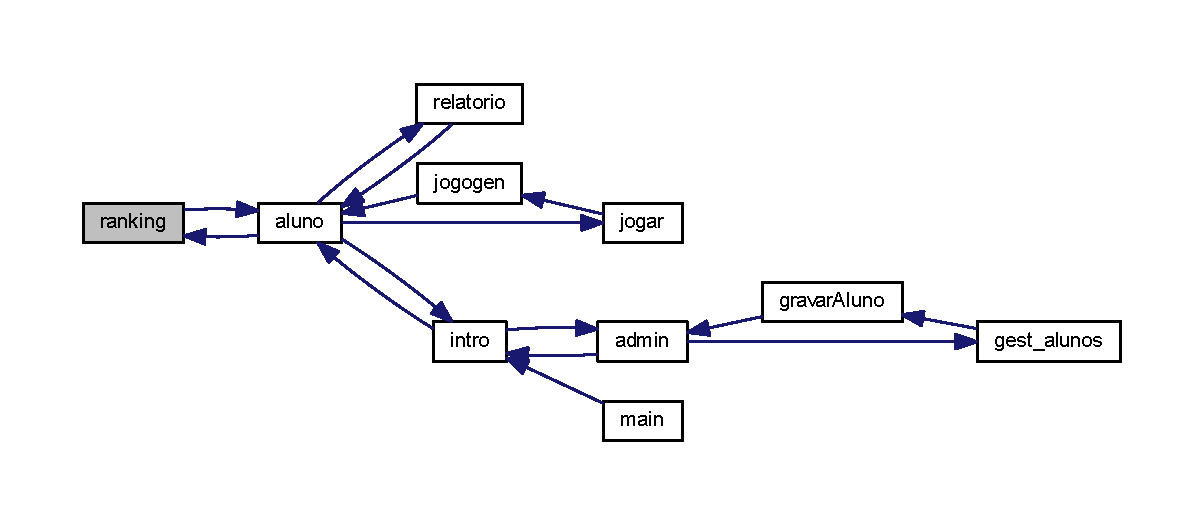
\includegraphics[width=350pt]{jogogen_8h_a9d5959cb84d9c4595414777c8b369a63_icgraph}
\end{center}
\end{figure}


\hypertarget{jogogen_8h_aa5261eb183e95885ae792f8ff46e3e53}{\index{jogogen.\+h@{jogogen.\+h}!relatorio@{relatorio}}
\index{relatorio@{relatorio}!jogogen.\+h@{jogogen.\+h}}
\subsubsection[{relatorio}]{\setlength{\rightskip}{0pt plus 5cm}void relatorio (
\begin{DoxyParamCaption}
\item[{int}]{iduser, }
\item[{{\bf alunotab} $\ast$}]{alu, }
\item[{char $\ast$}]{nome, }
\item[{int}]{indice}
\end{DoxyParamCaption}
)}}\label{jogogen_8h_aa5261eb183e95885ae792f8ff46e3e53}


Relatorio. 

funcao para relatorio de informa��o do aluno 
\begin{DoxyParams}{Parameters}
{\em iduser} & \+: int \\
\hline
{\em $\ast$alu} & \+: alunotab \\
\hline
{\em nome} & \+: $\ast$char \\
\hline
{\em indice} & \+: indice \\
\hline
\end{DoxyParams}
\begin{DoxyReturn}{Returns}
void 
\end{DoxyReturn}


Here is the call graph for this function\+:\nopagebreak
\begin{figure}[H]
\begin{center}
\leavevmode
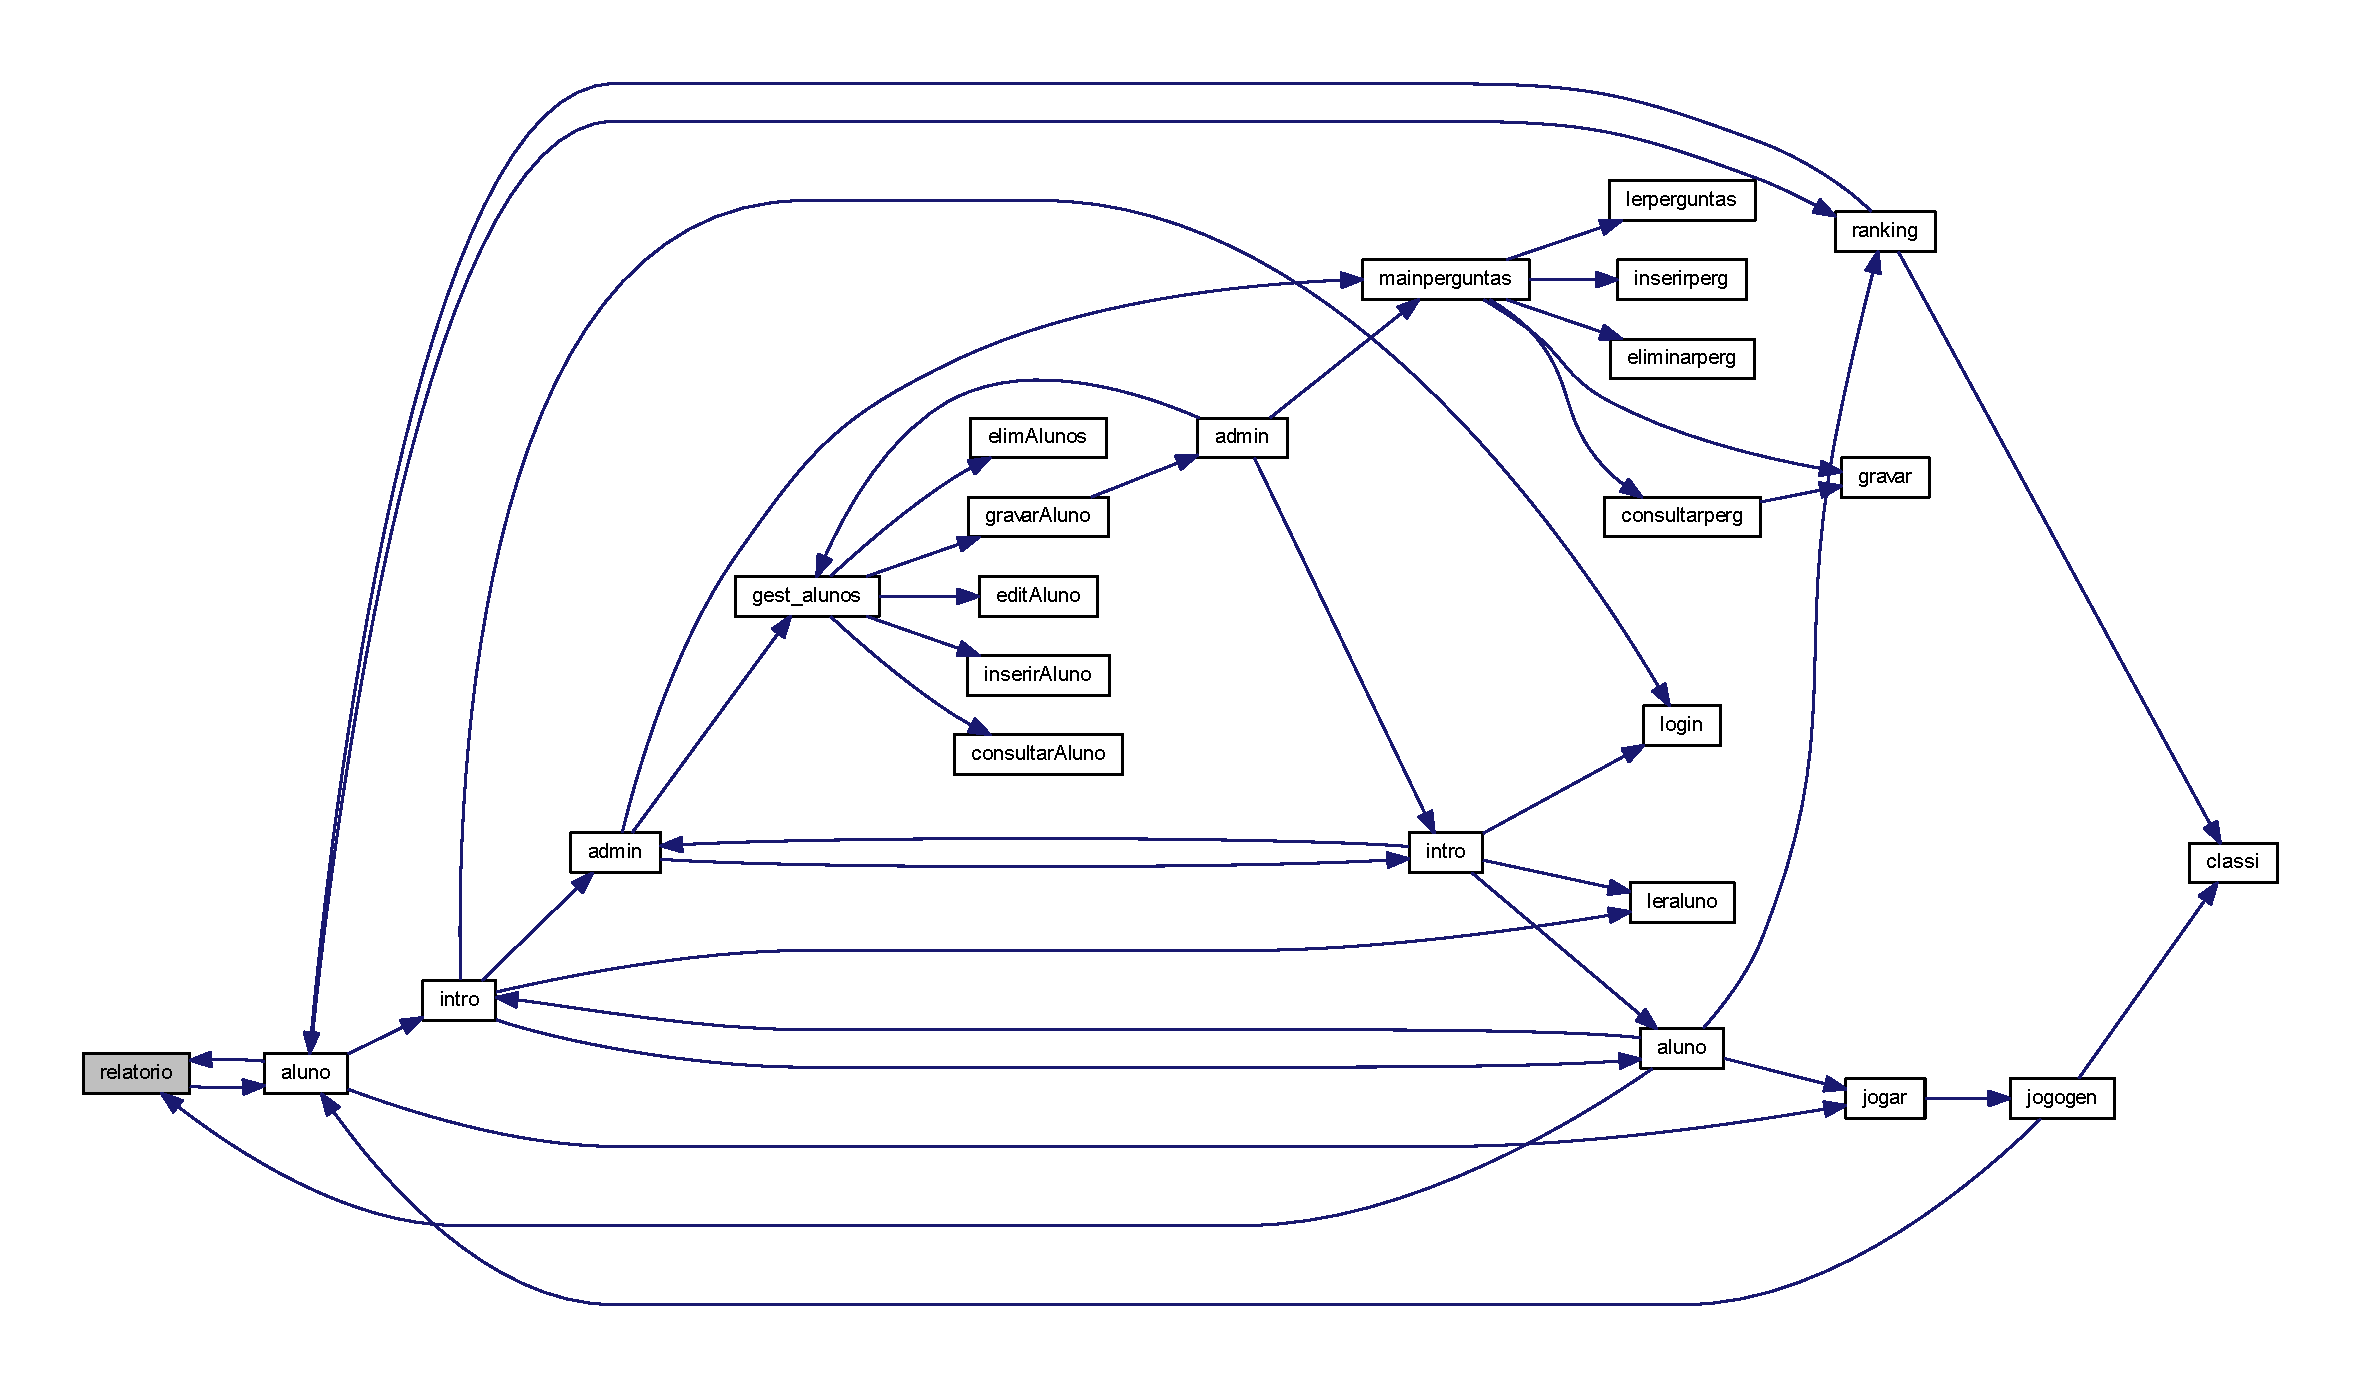
\includegraphics[width=350pt]{jogogen_8h_aa5261eb183e95885ae792f8ff46e3e53_cgraph}
\end{center}
\end{figure}




Here is the caller graph for this function\+:\nopagebreak
\begin{figure}[H]
\begin{center}
\leavevmode
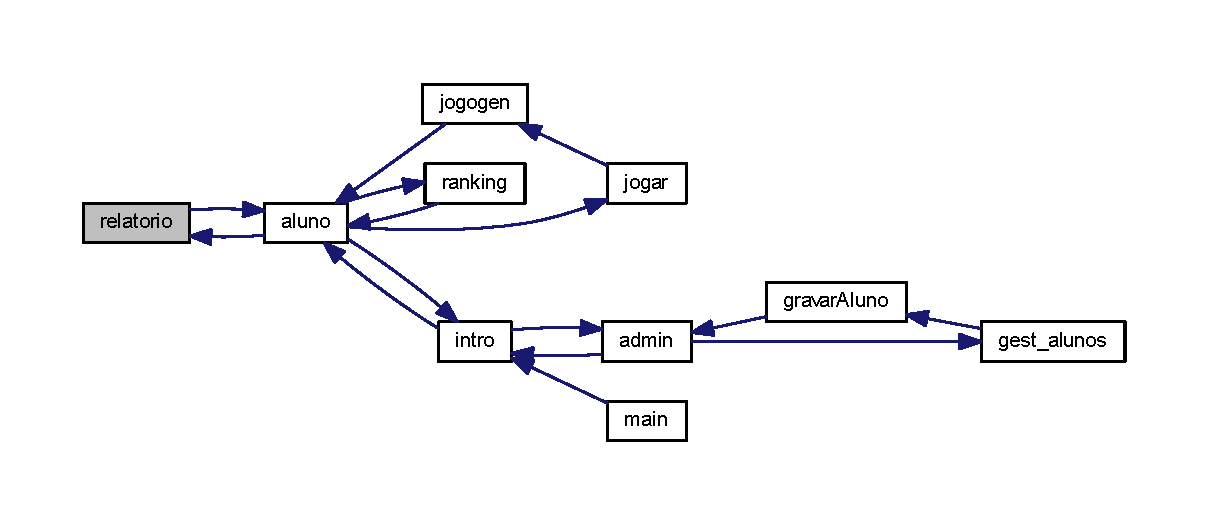
\includegraphics[width=350pt]{jogogen_8h_aa5261eb183e95885ae792f8ff46e3e53_icgraph}
\end{center}
\end{figure}



\hypertarget{login_8h}{\section{C\+:/\+Users/manuelseromenho/\+Desktop/quizmaster3001/source/login.h File Reference}
\label{login_8h}\index{C\+:/\+Users/manuelseromenho/\+Desktop/quizmaster3001/source/login.\+h@{C\+:/\+Users/manuelseromenho/\+Desktop/quizmaster3001/source/login.\+h}}
}


ficheiro login do Quizmaster 3001  


This graph shows which files directly or indirectly include this file\+:\nopagebreak
\begin{figure}[H]
\begin{center}
\leavevmode
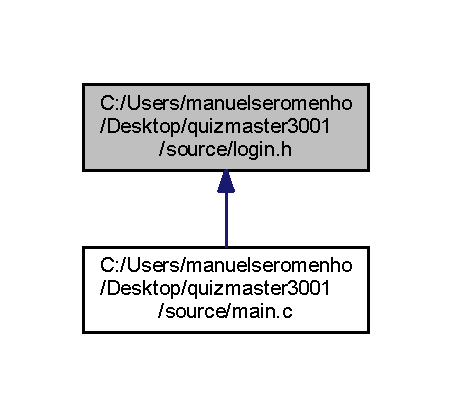
\includegraphics[width=217pt]{login_8h__dep__incl}
\end{center}
\end{figure}
\subsection*{Functions}
\begin{DoxyCompactItemize}
\item 
void \hyperlink{login_8h_a70c17e7e0c772226a81cccf10ff14a87}{aluno} (int iduser, \hyperlink{structalunotab}{alunotab} $\ast$alu)
\begin{DoxyCompactList}\small\item\em Menu aluno/user. \end{DoxyCompactList}\item 
void \hyperlink{login_8h_a0eac57f91f15716c9f3e15c935c69a8a}{admin} (\hyperlink{structalunotab}{alunotab} $\ast$alu)
\begin{DoxyCompactList}\small\item\em Menu Administrador. \end{DoxyCompactList}\item 
int \hyperlink{login_8h_a569aa668fcda751099ddec849b7938c3}{login} (int iduser, char password\mbox{[}15\mbox{]}, \hyperlink{structalunotab}{alunotab} $\ast$alu)
\begin{DoxyCompactList}\small\item\em Login. \end{DoxyCompactList}\item 
void \hyperlink{login_8h_a5ca8c98e0ec07103720da6e2b8241eac}{intro} (void)
\begin{DoxyCompactList}\small\item\em Menu de Login. \end{DoxyCompactList}\end{DoxyCompactItemize}


\subsection{Detailed Description}
ficheiro login do Quizmaster 3001 

instru��es para verificar o utilizador Quizmaster 3001 \begin{DoxyAuthor}{Author}
Manuel Seromenho 
\end{DoxyAuthor}
\begin{DoxyDate}{Date}
14 Janeiro 2015 
\end{DoxyDate}
\begin{DoxyRefDesc}{Bug}
\item[\hyperlink{bug__bug000004}{Bug}]sem erros detetados \begin{DoxyWarning}{Warning}
nenhum warning 
\end{DoxyWarning}
\begin{DoxyVersion}{Version}
1.\+0 
\end{DoxyVersion}
\begin{DoxyCopyright}{Copyright}
G\+N\+U Public License. 
\end{DoxyCopyright}
\end{DoxyRefDesc}


\subsection{Function Documentation}
\hypertarget{login_8h_a0eac57f91f15716c9f3e15c935c69a8a}{\index{login.\+h@{login.\+h}!admin@{admin}}
\index{admin@{admin}!login.\+h@{login.\+h}}
\subsubsection[{admin}]{\setlength{\rightskip}{0pt plus 5cm}void admin (
\begin{DoxyParamCaption}
\item[{{\bf alunotab} $\ast$}]{alu}
\end{DoxyParamCaption}
)}}\label{login_8h_a0eac57f91f15716c9f3e15c935c69a8a}


Menu Administrador. 

funcao do menu Administrador 
\begin{DoxyParams}{Parameters}
{\em $\ast$alu} & \+: alunotab \\
\hline
\end{DoxyParams}


Here is the call graph for this function\+:\nopagebreak
\begin{figure}[H]
\begin{center}
\leavevmode
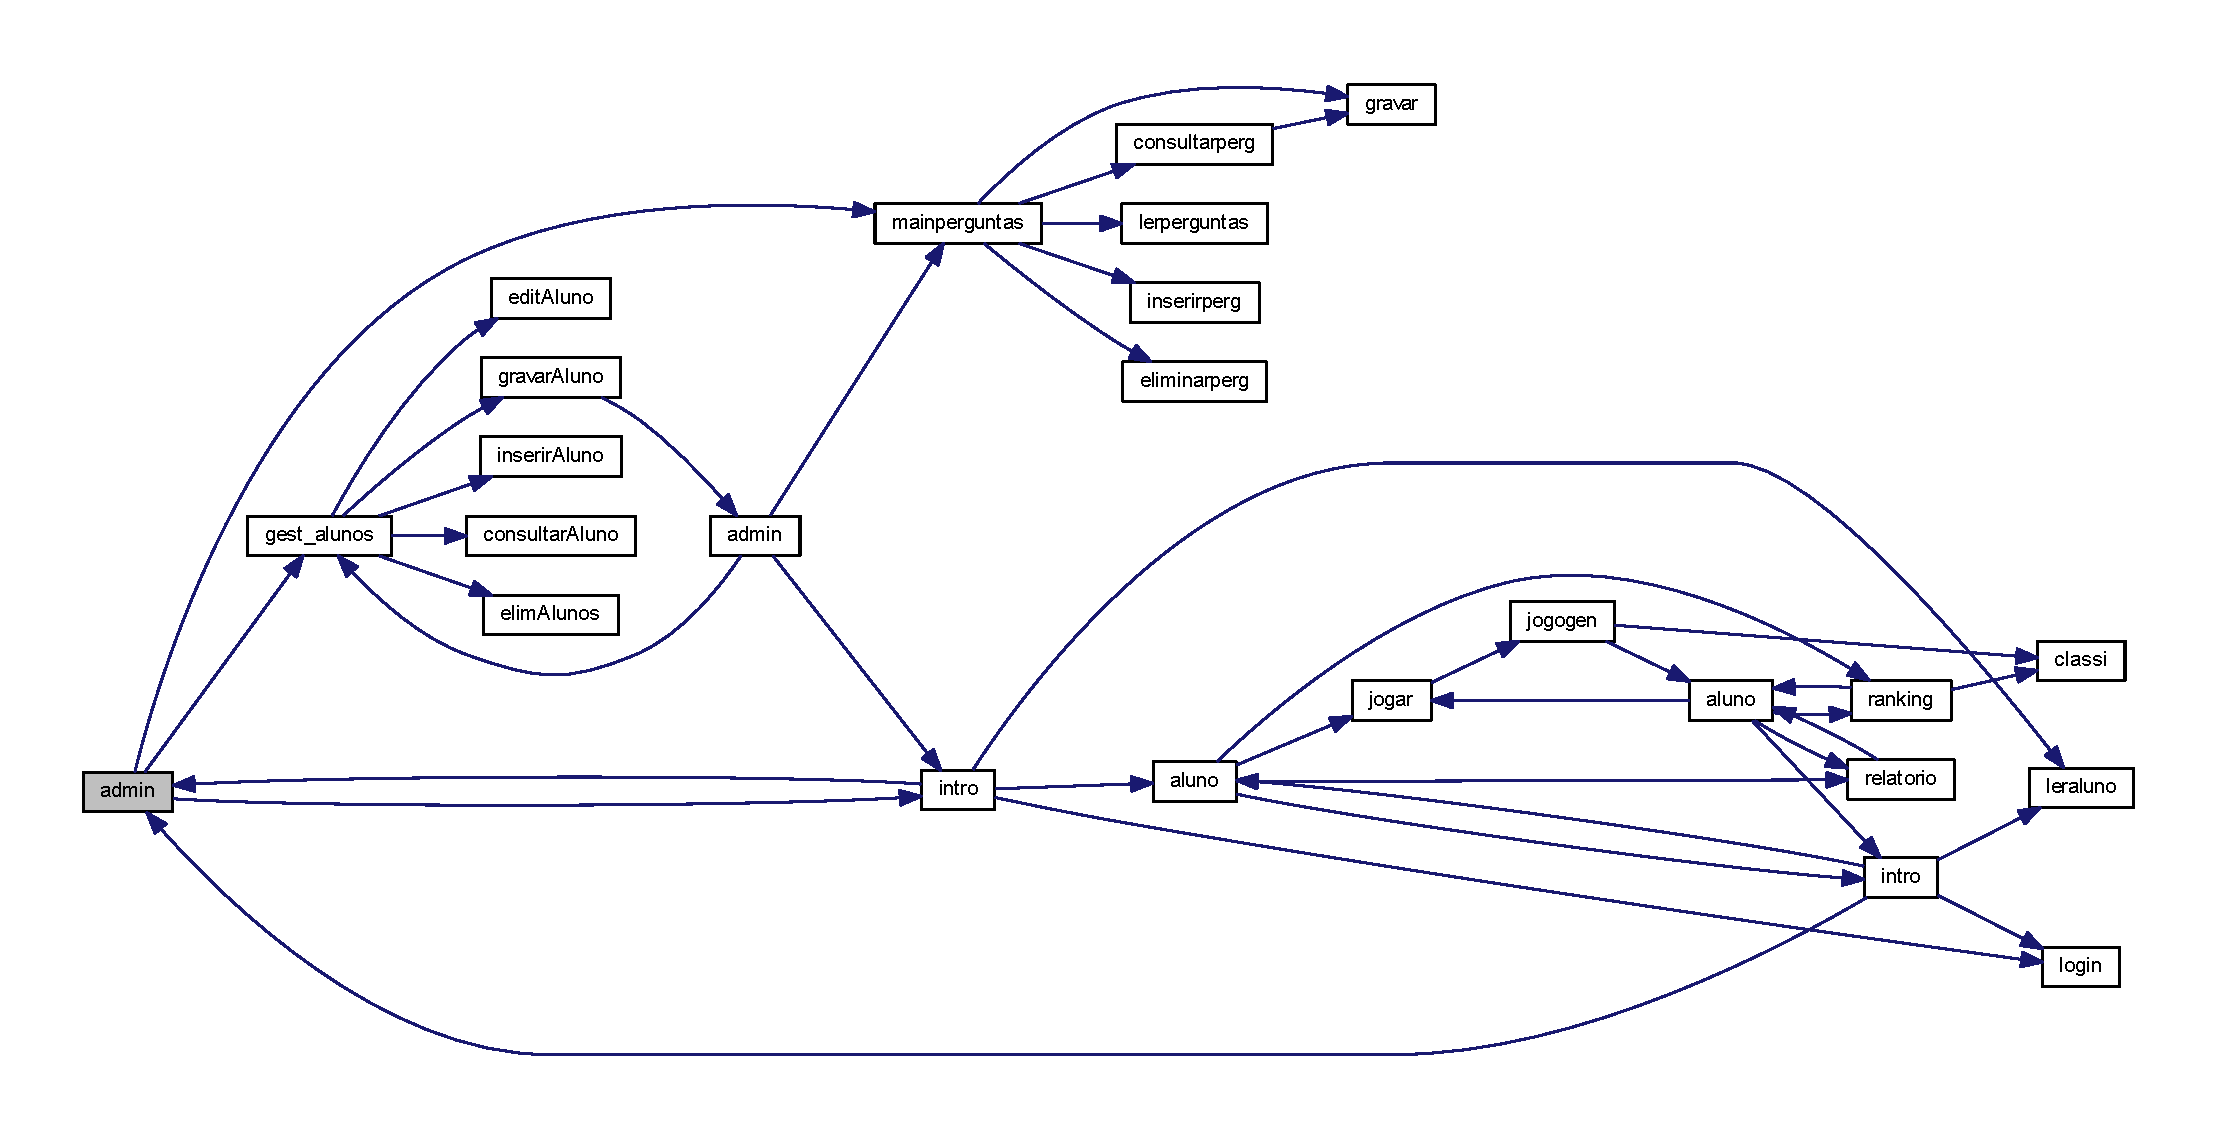
\includegraphics[width=350pt]{login_8h_a0eac57f91f15716c9f3e15c935c69a8a_cgraph}
\end{center}
\end{figure}




Here is the caller graph for this function\+:\nopagebreak
\begin{figure}[H]
\begin{center}
\leavevmode
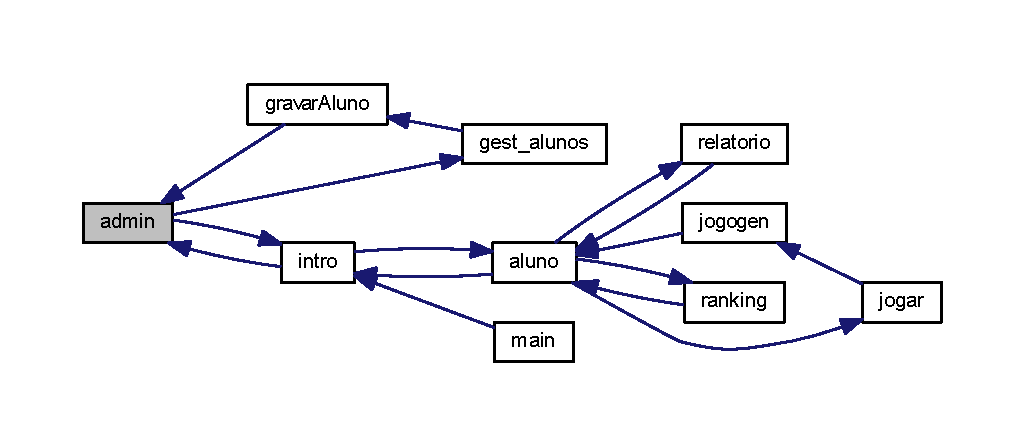
\includegraphics[width=350pt]{login_8h_a0eac57f91f15716c9f3e15c935c69a8a_icgraph}
\end{center}
\end{figure}


\hypertarget{login_8h_a70c17e7e0c772226a81cccf10ff14a87}{\index{login.\+h@{login.\+h}!aluno@{aluno}}
\index{aluno@{aluno}!login.\+h@{login.\+h}}
\subsubsection[{aluno}]{\setlength{\rightskip}{0pt plus 5cm}void aluno (
\begin{DoxyParamCaption}
\item[{int}]{iduser, }
\item[{{\bf alunotab} $\ast$}]{alu}
\end{DoxyParamCaption}
)}}\label{login_8h_a70c17e7e0c772226a81cccf10ff14a87}


Menu aluno/user. 

funcao menu aluno 
\begin{DoxyParams}{Parameters}
{\em iduser} & \+: int \\
\hline
{\em $\ast$alu} & \+: alunotab \\
\hline
\end{DoxyParams}
\begin{DoxyReturn}{Returns}
void 
\end{DoxyReturn}


Here is the call graph for this function\+:\nopagebreak
\begin{figure}[H]
\begin{center}
\leavevmode
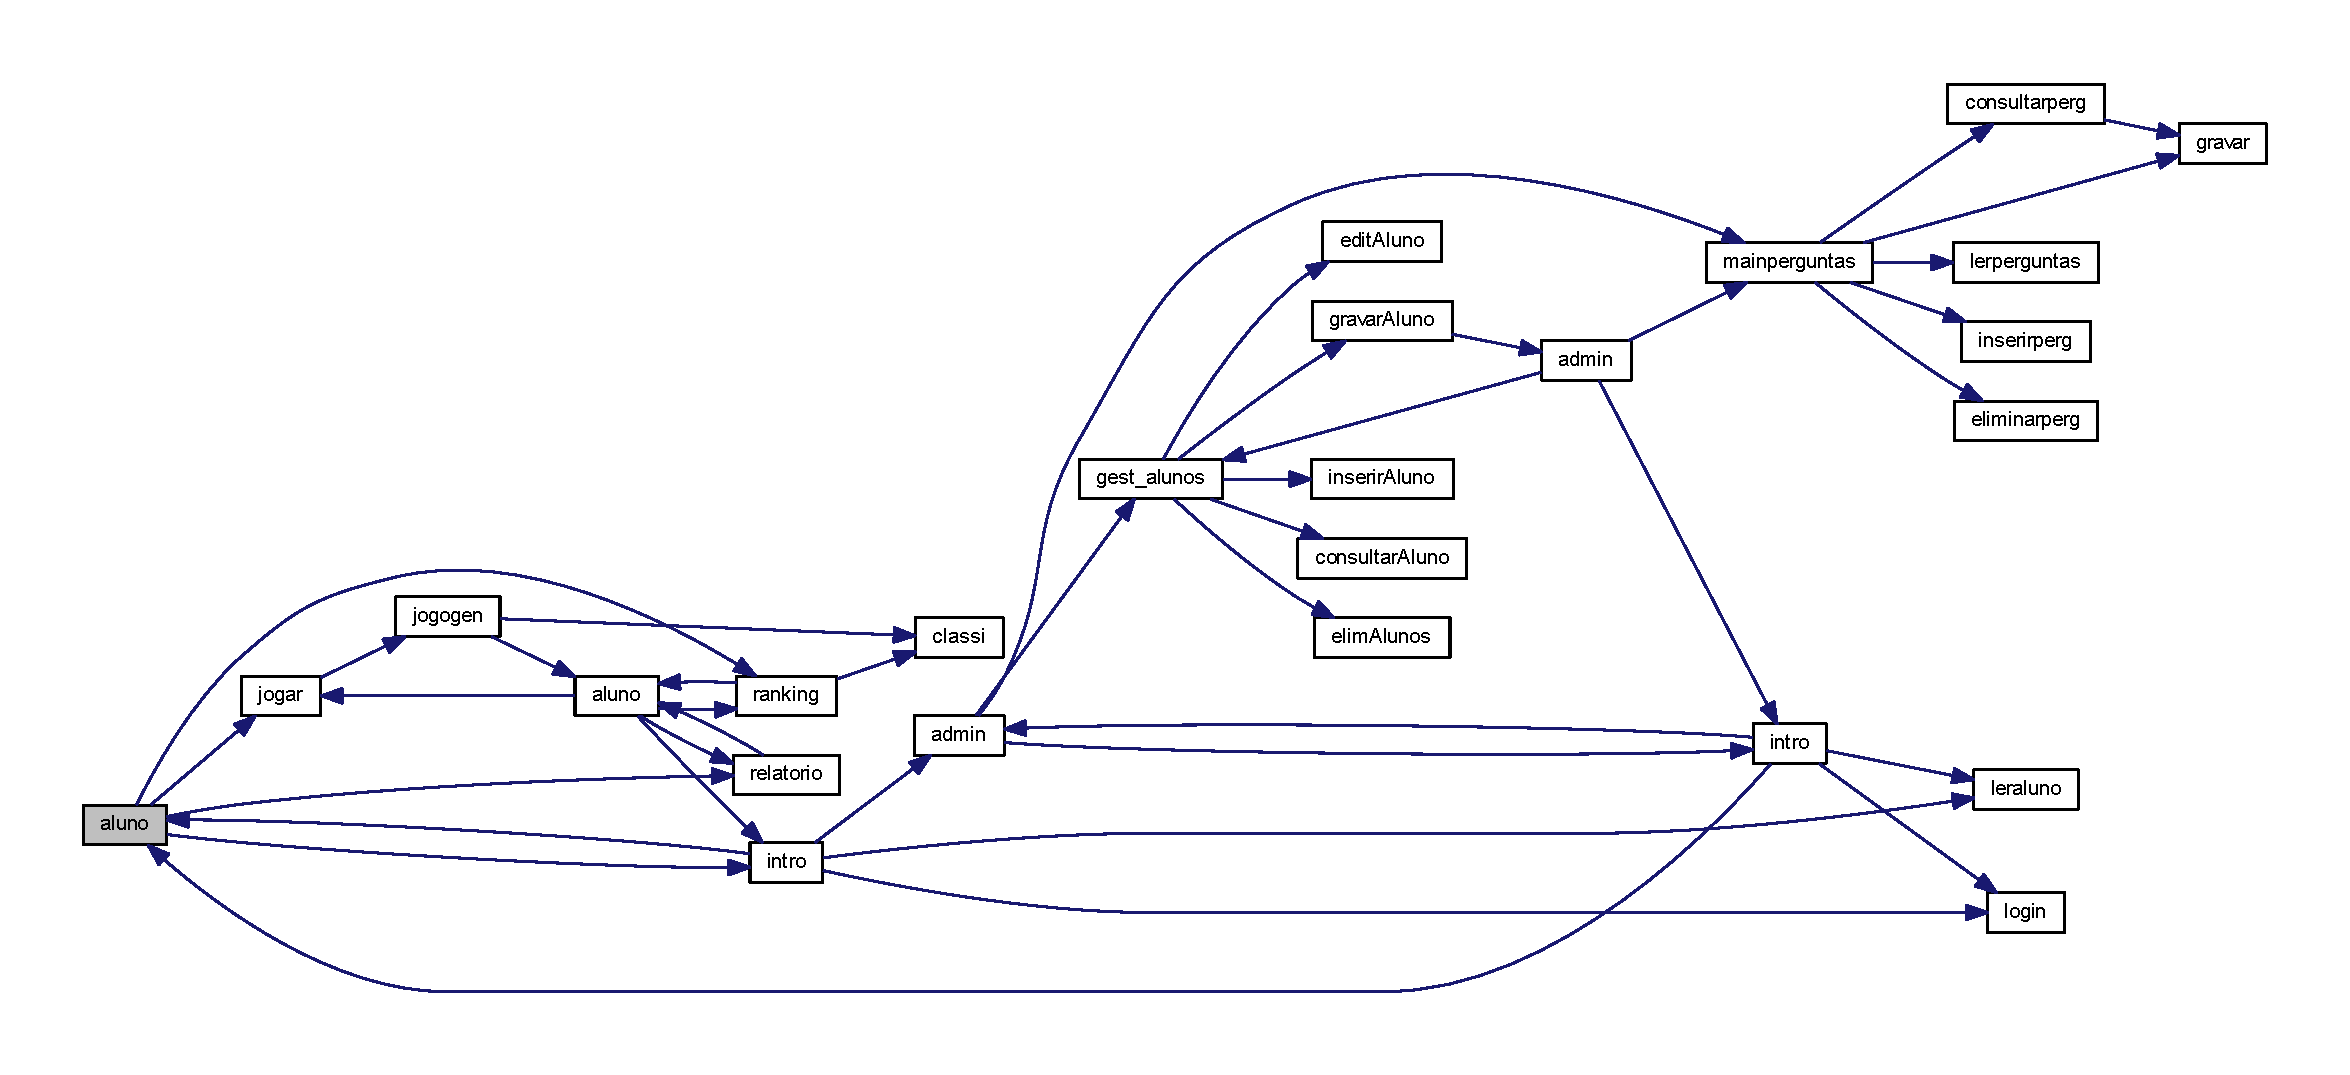
\includegraphics[width=350pt]{login_8h_a70c17e7e0c772226a81cccf10ff14a87_cgraph}
\end{center}
\end{figure}




Here is the caller graph for this function\+:\nopagebreak
\begin{figure}[H]
\begin{center}
\leavevmode
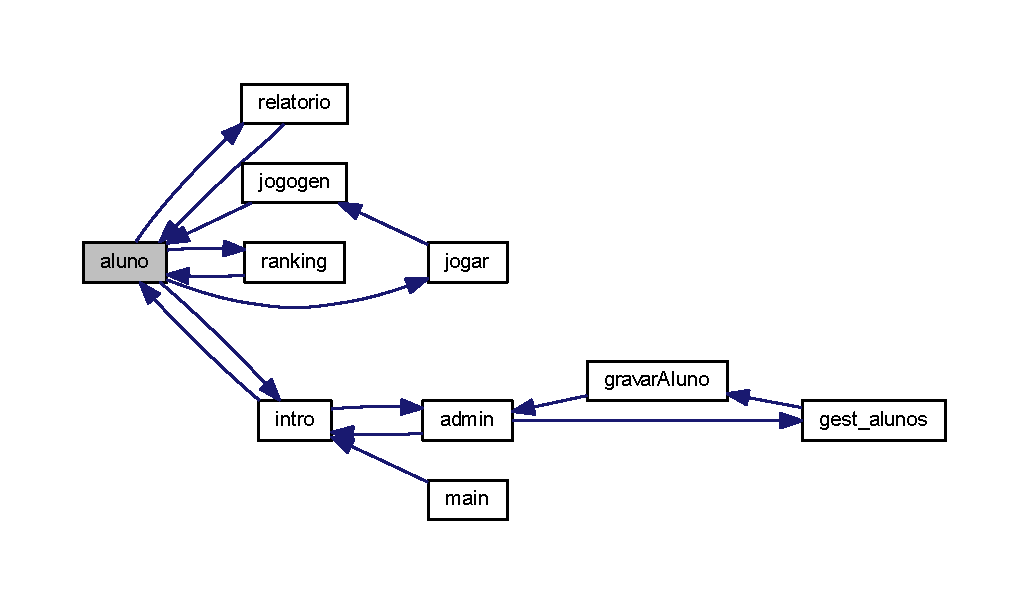
\includegraphics[width=350pt]{login_8h_a70c17e7e0c772226a81cccf10ff14a87_icgraph}
\end{center}
\end{figure}


\hypertarget{login_8h_a5ca8c98e0ec07103720da6e2b8241eac}{\index{login.\+h@{login.\+h}!intro@{intro}}
\index{intro@{intro}!login.\+h@{login.\+h}}
\subsubsection[{intro}]{\setlength{\rightskip}{0pt plus 5cm}void intro (
\begin{DoxyParamCaption}
\item[{void}]{}
\end{DoxyParamCaption}
)}}\label{login_8h_a5ca8c98e0ec07103720da6e2b8241eac}


Menu de Login. 

funcao do Menu de Login (onde os users/alunos introduzem a informa��o para ser verificada pela fun��o login) 

Here is the call graph for this function\+:\nopagebreak
\begin{figure}[H]
\begin{center}
\leavevmode
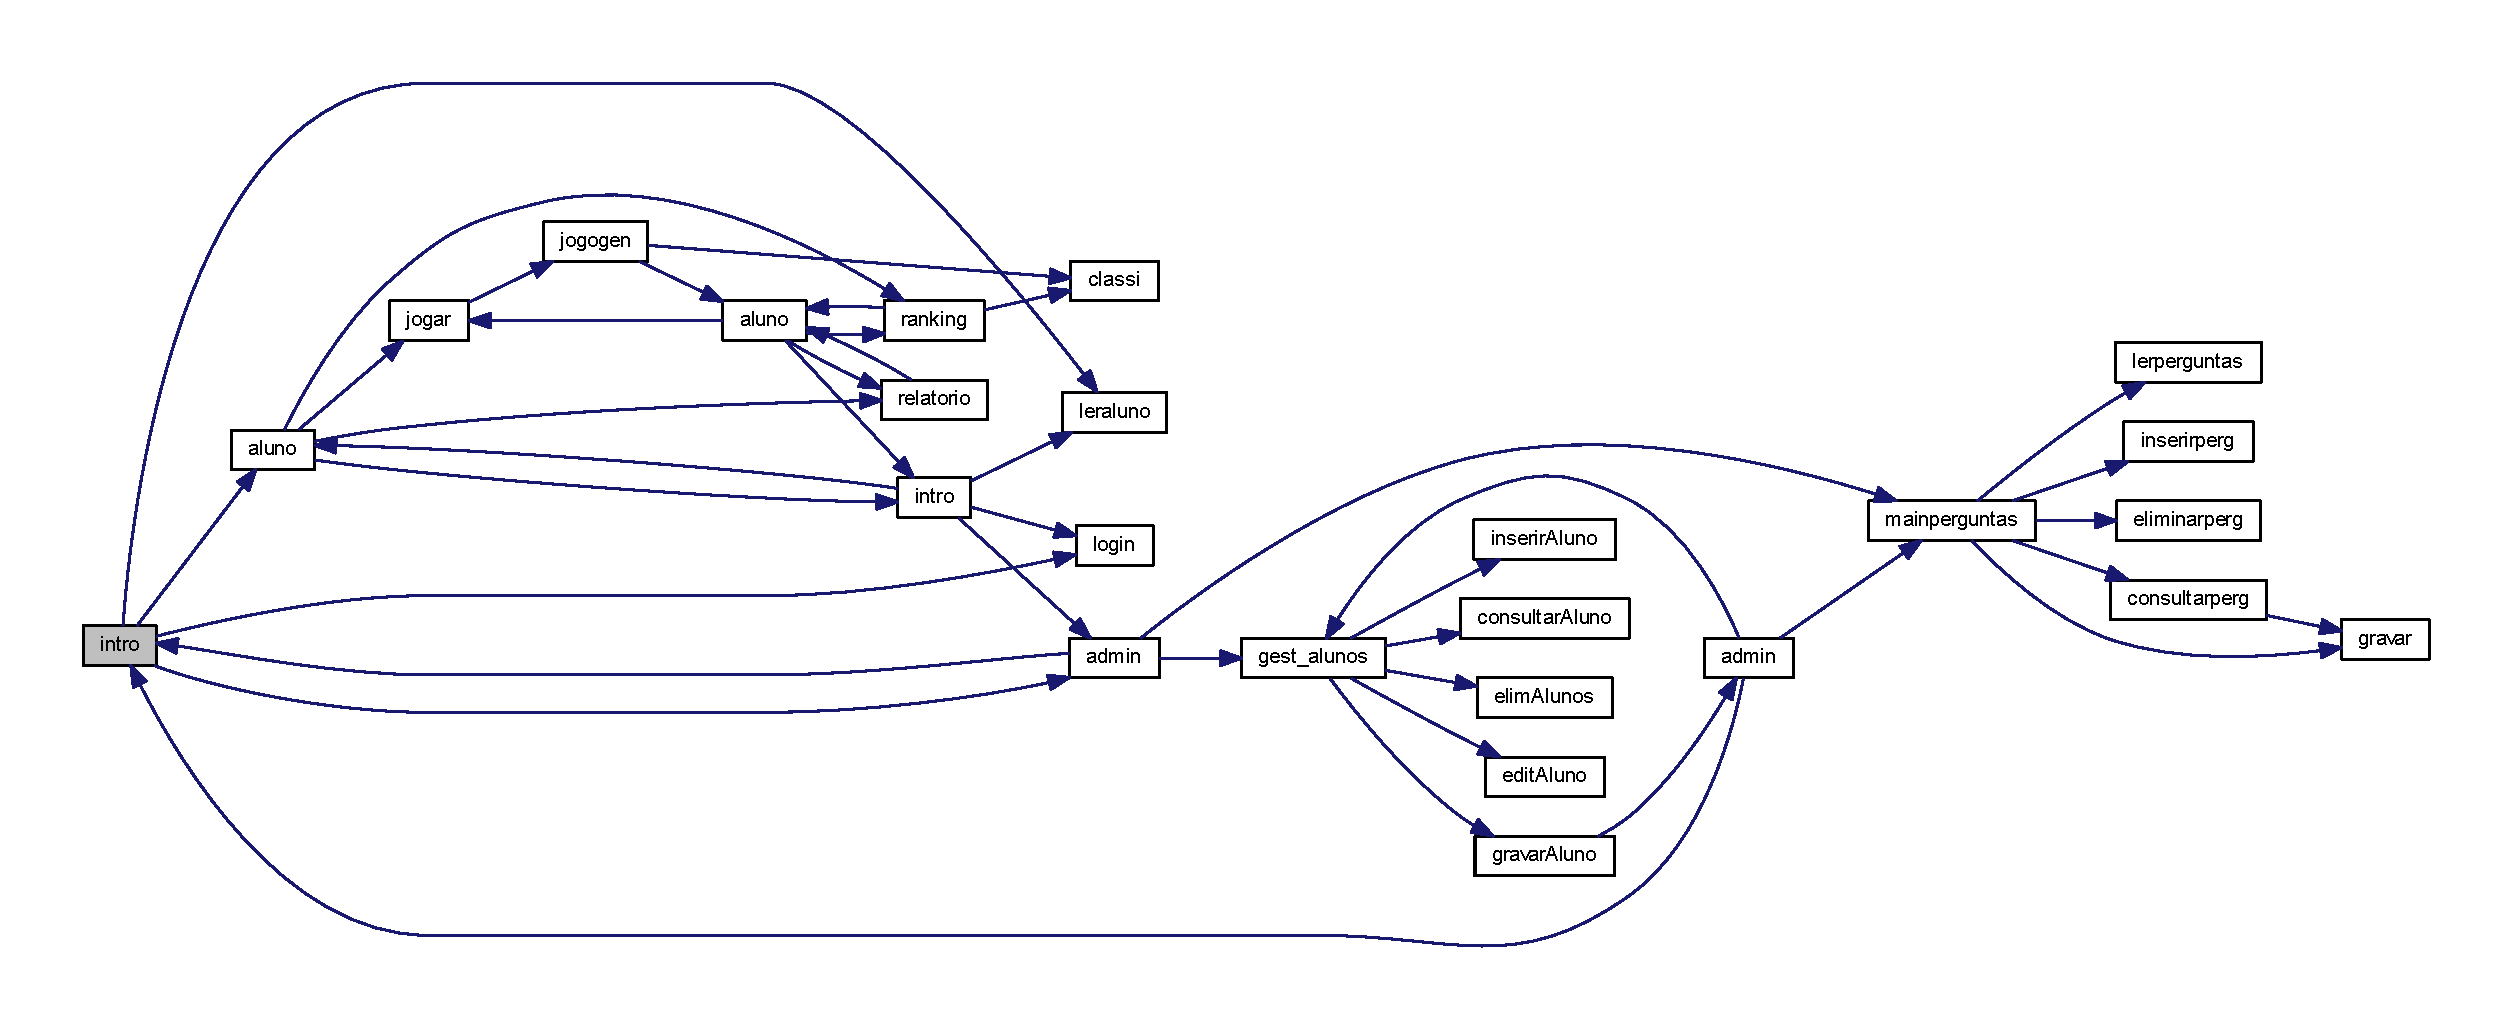
\includegraphics[width=350pt]{login_8h_a5ca8c98e0ec07103720da6e2b8241eac_cgraph}
\end{center}
\end{figure}




Here is the caller graph for this function\+:\nopagebreak
\begin{figure}[H]
\begin{center}
\leavevmode
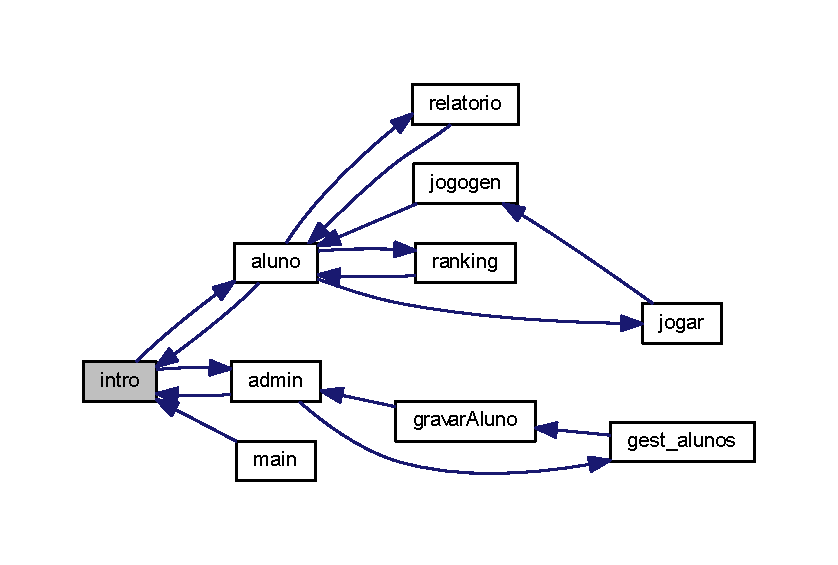
\includegraphics[width=350pt]{login_8h_a5ca8c98e0ec07103720da6e2b8241eac_icgraph}
\end{center}
\end{figure}


\hypertarget{login_8h_a569aa668fcda751099ddec849b7938c3}{\index{login.\+h@{login.\+h}!login@{login}}
\index{login@{login}!login.\+h@{login.\+h}}
\subsubsection[{login}]{\setlength{\rightskip}{0pt plus 5cm}int login (
\begin{DoxyParamCaption}
\item[{int}]{iduser, }
\item[{char}]{password\mbox{[}15\mbox{]}, }
\item[{{\bf alunotab} $\ast$}]{alu}
\end{DoxyParamCaption}
)}}\label{login_8h_a569aa668fcda751099ddec849b7938c3}


Login. 

funcao para Login dos Users/\+Alunos 
\begin{DoxyParams}{Parameters}
{\em iduser} & \+: int \\
\hline
{\em password} & \+: char \\
\hline
{\em $\ast$alu} & \+: alunotab \\
\hline
\end{DoxyParams}
\begin{DoxyReturn}{Returns}
login\+: int 
\end{DoxyReturn}


Here is the caller graph for this function\+:\nopagebreak
\begin{figure}[H]
\begin{center}
\leavevmode
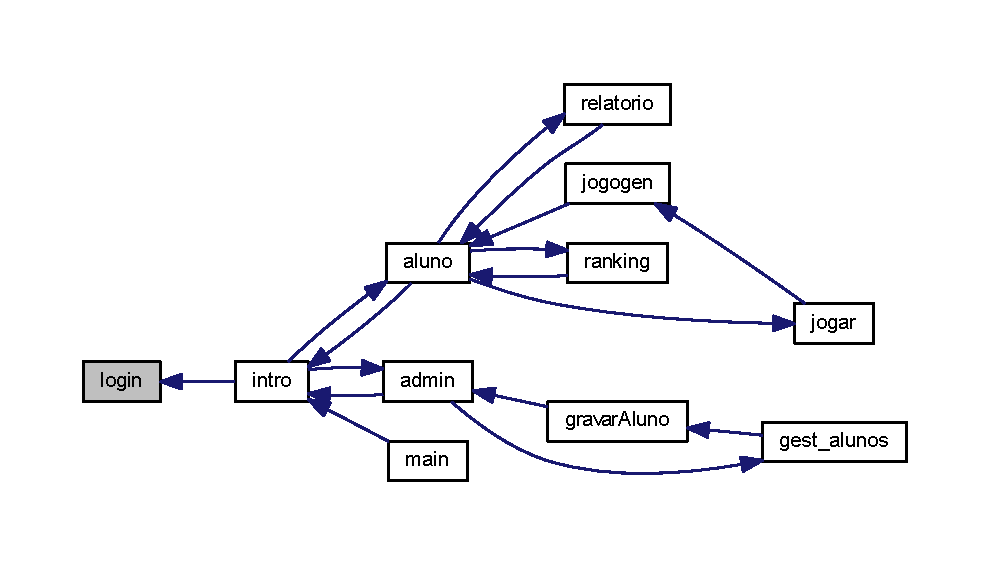
\includegraphics[width=350pt]{login_8h_a569aa668fcda751099ddec849b7938c3_icgraph}
\end{center}
\end{figure}



\hypertarget{main_8c}{\section{C\+:/\+Users/manuelseromenho/\+Desktop/quizmaster3001/source/main.c File Reference}
\label{main_8c}\index{C\+:/\+Users/manuelseromenho/\+Desktop/quizmaster3001/source/main.\+c@{C\+:/\+Users/manuelseromenho/\+Desktop/quizmaster3001/source/main.\+c}}
}


ficheiro main do Quizmaster 3001  


{\ttfamily \#include \char`\"{}includes\+\_\+defines.\+h\char`\"{}}\\*
{\ttfamily \#include \char`\"{}estruturas.\+h\char`\"{}}\\*
{\ttfamily \#include \char`\"{}admin\+\_\+perguntas.\+h\char`\"{}}\\*
{\ttfamily \#include \char`\"{}admin\+\_\+aluno.\+h\char`\"{}}\\*
{\ttfamily \#include \char`\"{}login.\+h\char`\"{}}\\*
{\ttfamily \#include \char`\"{}jogogen.\+h\char`\"{}}\\*
Include dependency graph for main.\+c\+:\nopagebreak
\begin{figure}[H]
\begin{center}
\leavevmode
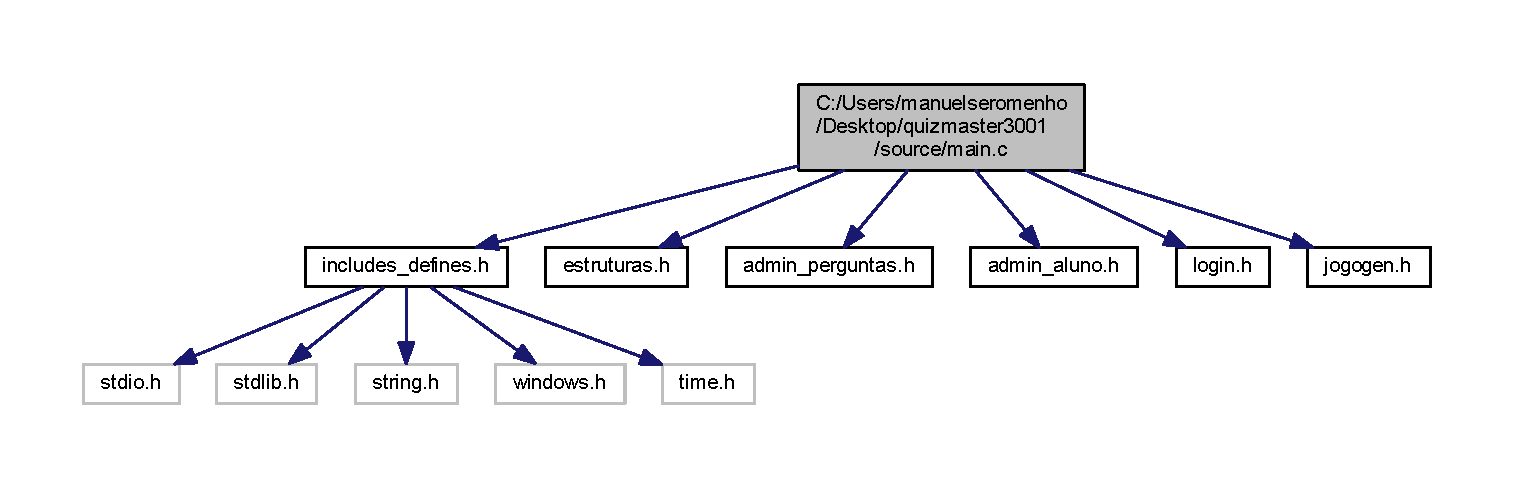
\includegraphics[width=350pt]{main_8c__incl}
\end{center}
\end{figure}
\subsection*{Functions}
\begin{DoxyCompactItemize}
\item 
\hyperlink{main_8c_a51af30a60f9f02777c6396b8247e356f}{main} ()
\end{DoxyCompactItemize}


\subsection{Detailed Description}
ficheiro main do Quizmaster 3001 

primeiras instru��es do programa Quizmaster 3001 \begin{DoxyAuthor}{Author}
Manuel Seromenho 
\end{DoxyAuthor}
\begin{DoxyDate}{Date}
14 Janeiro 2015 
\end{DoxyDate}
\begin{DoxyRefDesc}{Bug}
\item[\hyperlink{bug__bug000005}{Bug}]sem erros detetados \begin{DoxyWarning}{Warning}
nenhum warning 
\end{DoxyWarning}
\begin{DoxyVersion}{Version}
1.\+0 
\end{DoxyVersion}
\begin{DoxyCopyright}{Copyright}
G\+N\+U Public License. 
\end{DoxyCopyright}
\end{DoxyRefDesc}


\subsection{Function Documentation}
\hypertarget{main_8c_a51af30a60f9f02777c6396b8247e356f}{\index{main.\+c@{main.\+c}!main@{main}}
\index{main@{main}!main.\+c@{main.\+c}}
\subsubsection[{main}]{\setlength{\rightskip}{0pt plus 5cm}main (
\begin{DoxyParamCaption}
{}
\end{DoxyParamCaption}
)}}\label{main_8c_a51af30a60f9f02777c6396b8247e356f}


Here is the call graph for this function\+:\nopagebreak
\begin{figure}[H]
\begin{center}
\leavevmode
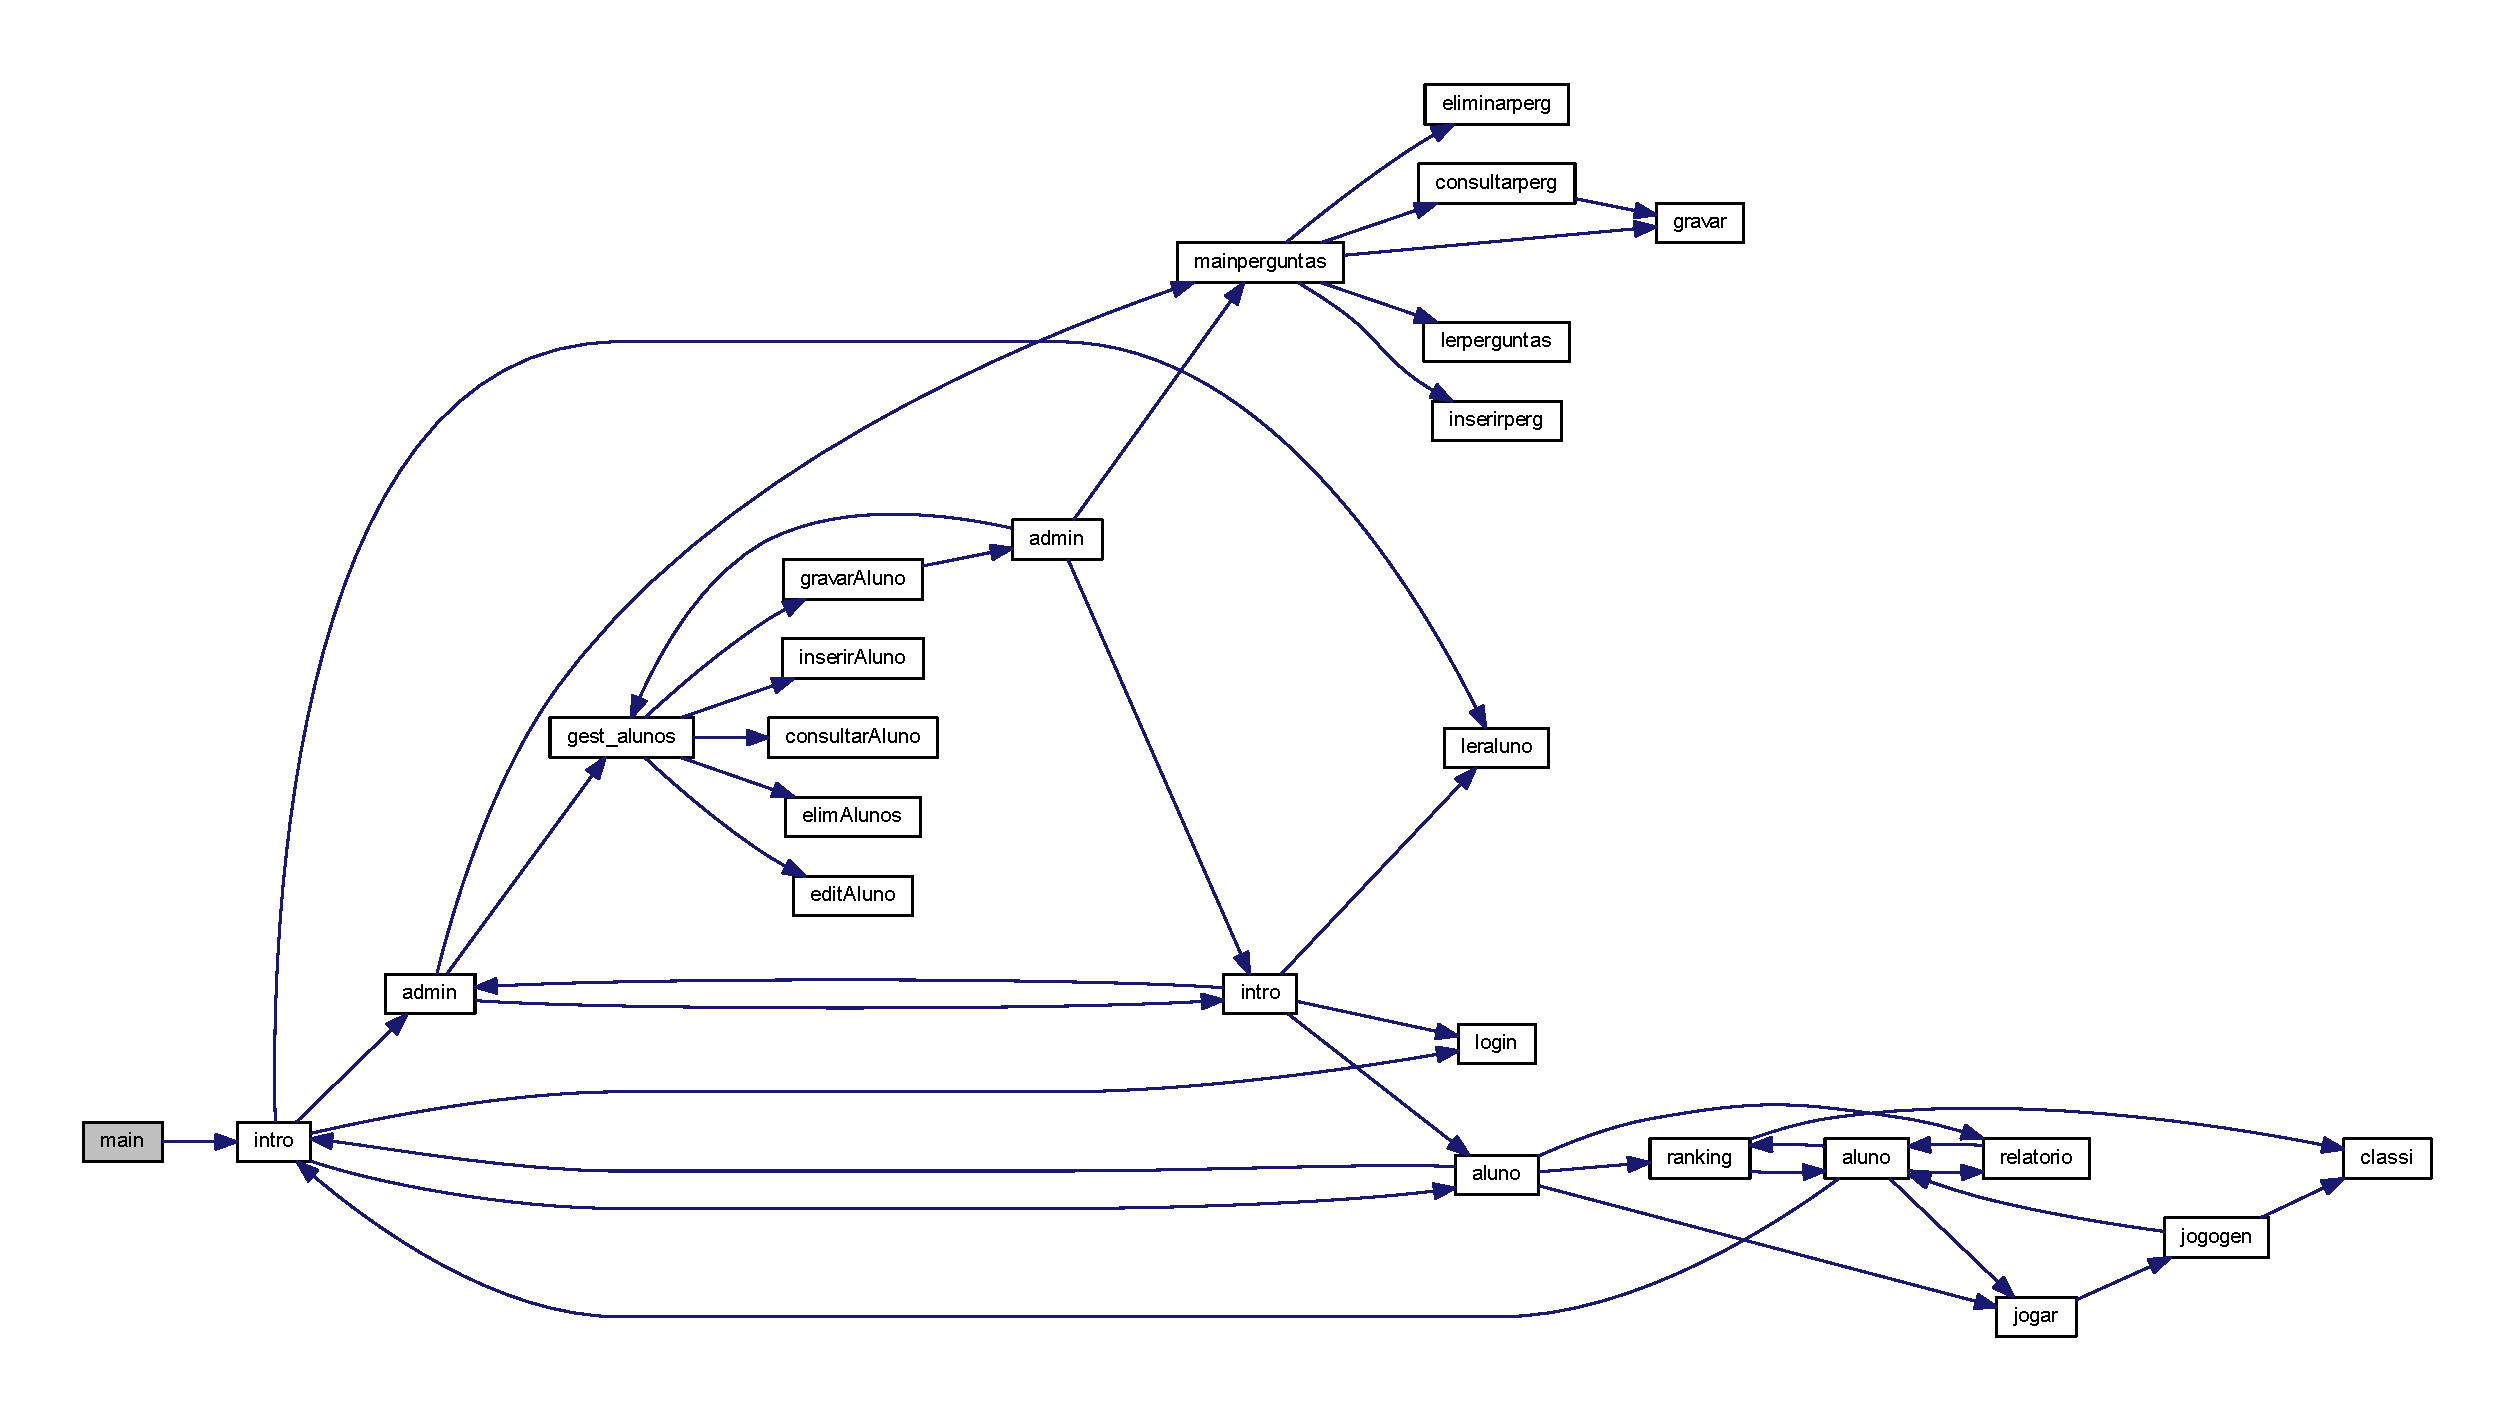
\includegraphics[width=350pt]{main_8c_a51af30a60f9f02777c6396b8247e356f_cgraph}
\end{center}
\end{figure}



\hypertarget{_r_e_a_d_m_e_8md}{\section{C\+:/\+Users/manuelseromenho/\+Desktop/quizmaster3001/source/\+R\+E\+A\+D\+M\+E.md File Reference}
\label{_r_e_a_d_m_e_8md}\index{C\+:/\+Users/manuelseromenho/\+Desktop/quizmaster3001/source/\+R\+E\+A\+D\+M\+E.\+md@{C\+:/\+Users/manuelseromenho/\+Desktop/quizmaster3001/source/\+R\+E\+A\+D\+M\+E.\+md}}
}

%--- End generated contents ---

% Index
\newpage
\phantomsection
\addcontentsline{toc}{chapter}{Index}
\printindex

\end{document}
